%---------------------------------------------------------------------------%
%-                                                                         -%
%-                           LaTeX Template                                -%
%-                                                                         -%
%---------------------------------------------------------------------------%
%- Copyright (C) Huangrui Mo <huangrui.mo@gmail.com> 
%- This is free software: you can redistribute it and/or modify it
%- under the terms of the GNU General Public License as published by
%- the Free Software Foundation, either version 3 of the License, or
%- (at your option) any later version.
%---------------------------------------------------------------------------%
%->> Document class declaration
%---------------------------------------------------------------------------%
\documentclass[doublesided]{Style/ucasthesis}%
%- Multiple optional arguments:
%- [<singlesided|doublesided|printcopy>]% set one or two sided eprint or print
%- [draftversion]% show draft version information
%- [fontset=<fandol|...>]% specify font set to replace automatic detection
%- [scheme=plain]% thesis writing of international students
%- [standard options for ctex book class: draft|paper size|font size|...]%
%---------------------------------------------------------------------------%
%->> Document settings
%---------------------------------------------------------------------------%
%\usepackage[authoryear,myhdr,list]{Style/artratex}% document settings
%\usepackage[super,myhdr,list]{Style/artratex}% document settings
\usepackage[numbers,myhdr,list]{Style/artratex}% document settings
%- usage: \usepackage[option1,option2,...,optionN]{artratex}
%- Multiple optional arguments:
%- [bibtex|biber]% set bibliography processor and package
%- [<numbers|super|authoryear|alpha>]% set citation and reference style
%- <numbers>: textual: Jones [1]; parenthetical: [1]
%- <super>: textual: Jones superscript [1]; parenthetical: superscript [1]
%- <authoryear>: textual: Jones (1995); parenthetical: (Jones, 1995)
%- <alpha>: textual: not available; parenthetical: [Jon95]
%- [geometry]% reconfigure page layout via geometry package
%- [lscape]% provide landscape layout environment
%- [myhdr]% enable header and footer via fancyhdr package
%- [color]% provide color support via xcolor package
%- [background]% enable page background
%- [tikz]% provide complex diagrams via tikz package
%- [table]% provide complex tables via ctable package
%- [list]% provide enhanced list environments for algorithm and coding
%- [math]% enable some extra math packages
\usepackage{Style/artracom}% user defined commands
%---------------------------------------------------------------------------%
%->> Document inclusion
%---------------------------------------------------------------------------%
%\includeonly{Tex/Chap_1,...,Tex/Chap_N}% selected files compilation
%---------------------------------------------------------------------------%
%->> Document content
%---------------------------------------------------------------------------%
\begin{document}
%-
%-> Frontmatter: title page, abstract, content list, symbol list, preface
%-
\frontmatter% initialize the environment
%---------------------------------------------------------------------------%
%->> 封面信息及生成
%---------------------------------------------------------------------------%
%-
%-> 中文封面信息
%-
\confidential{}% 密级:只有涉密论文才填写
\schoollogo{scale=0.095}{ucas_logo}% 校徽
\title{BESIII实验上粲重子{$\Lambda^+_c\to\Xi^{(*)0}K^+$} 绝对衰变分支比测量及{$\lhcb$}实验上质心系能量在13{$\tev$}下{$\psitwos$}产生截面测量}
\author{李培荣}
\advisor{郑阳恒~教授,~中国科学院大学}
\advisorsec{}% 指导老师附加信息 或 第二指导老师信息
\degree{物理学}% 学位:学士、硕士、博士
\degreetype{地球}% 学位类别:理学、工学、工程、医学等
\major{粒子物理与原子核物理}
\institute{中国科学院大学物理科学学院}
\chinesedate{2018~年~7~月}% 毕业日期:夏季为6月、冬季为12月
%-
%-> 英文封面信息
%-
\englishtitle{Measurements of Absolute  Branching Fractions for {$\Lambda^+_c\to\Xi^{(*)0}K^+$} \\ at BESII and \\ Measurement of {$\psitwos$} production cross-sections at {\lhcb} at 13{$\tev$}} 
\englishauthor{Pei-Rong Li}
\englishadvisor{Prof. Yangheng Zheng}
\englishdegree{Doctor}% 学位:Bachelor, Master, Doctor。封面格式将根据英文学位名称自动切换,请确保拼写准确无误
\englishdegreetype{Natural Science}% 学位类别:Philosophy, Natural Science, Engineering, Economics, Agriculture 等
\englishthesistype{thesis}% 论文类型: thesis, dissertation
\englishmajor{Particle Physics and Nuclear Physics}% 二级学科专业名称
\englishinstitute{University of Chinese Academy of Sciences}
\englishdate{July, 2018}% 毕业日期:夏季为June、冬季为December

%-
%-> 生成封面
%-
\maketitle% 生成中文封面
\makeenglishtitle% 生成英文封面
%-
%-> 作者声明
%-
\makedeclaration% 生成声明页
%-
%-> 中文摘要
%-
\chapter*{摘\quad 要}\chaptermark{摘\quad 要}% 摘要标题
\setcounter{page}{1}% 开始页码
\pagenumbering{Roman}% 页码符号

粲重子$\lambdacp$的强子末态衰变只能通过弱相互作用发生,研究其衰变分支比对于理解弱相互作用十分重要。
基于BESIII实验在 $\sqrt{s}=4.6\gev$ 处采集的567\,pb$^{-1}$的~$\ee$~对撞数据,运用双$\Lambda_c$标记的技术首次测量了$\Lambda^+_c\to\Xi^{(*)0}K^+$的绝对分支比分别为$\mathcal{B}(\Lambda^+_c\to\Xi^0K^+)=(5.90\pm0.86\pm0.39)\times10^{-3}$~和~$\mathcal{B}(\Lambda^+_c\to\Xi(1530)^0K^+)=(5.02\pm0.99\pm0.31)\times10^{-3}$。
其中第一项误差指的是统计误差,第二项为系统误差。
这一测量是首次进行的绝对测量,且结果同之前相对测量的精度要好。

利用大型强子对撞机$\lhc$上的$\lhcb$实验在2015年收集的积分亮度为275\,pb$^{-1}$的质子-质子对撞数据,我们对$\psitwos$介子的微分产生截面进行了测量。
对于直接产生的$\psitwos$介子和来自于$b$强子衰变的$\psitwos$介子我们都测量了其在横动量范围$2<\pt<20\gevc$且快度范围$2.0<y<4.5$区间内,产生截面随着横动量$\pt$和快度$y$变化的微分截面。
在整个运动学区间内的积分截面对于直接产生的$\psitwos$介子为$\promptresult$,对于来自于$b$强子衰变的$\psitwos$介子为$\frombresult$。
其中第一项误差指的是统计误差,第二项为系统误差。
上述所有的测量结果都和理论计算吻合的很好。

\keywords{北京谱仪III,粲重子$\Lambda_c^+$,绝对分支比,$\lhcb$,$\psitwos$介子,产生截面}
%-
%-> 英文摘要
%-
\chapter*{Abstract}\chaptermark{Abstract}% 摘要标题

The hadronic decays of charmed baryon $\lambdacp$ happen only through weak interaction.
The study of its hadronic decay rates are key probes to understand the weak interactions.
We report the first measurements of absolute branching fractions for the $W$-exchange-only processes $\Lambda^+_c\to\Xi^0K^+$ and $\Lambda^+_c\to\Xi(1530)^0K^+$ with the double-tag technique, by analyzing an $e^{+}e^{-}$ collision data sample, that corresponds to an integrated luminosity of 567~pb$^{-1}$ collected at a centre-of-mass energy of 4.6~GeV by the BESIII detector.
The branching fractions are measured to be $\mathcal{B}(\Lambda^+_c\to\Xi^0K^+)=(5.90\pm0.86\pm0.39)\times10^{-3}$ and $\mathcal{B}(\Lambda^+_c\to\Xi(1530)^0K^+)=(5.02\pm0.99\pm0.31)\times10^{-3}$, where the first uncertainties are statistical and the second systematic.
These are the first absolute measurements of their branching fractions and the precisions are also improved compared with the relative measurements before.

The production cross-sections of $\psitwos$ mesons in proton-proton collisions at a centre-of-mass energy $\sqs=13\tev$ are measured with a data sample collected by the $\lhcb$ detector in the $\lhc$ operations in 2015. 
The corresponding integrated luminosity is $275\invpb$.
 The cross-sections for prompt $\psitwos$ mesons and those for $\psitwos$ mesons from $b$-hadron decays are determined as functions of the transverse momentum $\pt$ and the rapidity $y$ of the $\psitwos$ meson in the kinematic range $2<\pt<20\gevc$ and $2.0<y<4.5$.
The production cross-sections integrated over the kinematic coverage are 
$\promptresult$ 
%$1.497\pm0.004\stat\pm0.082\syst\mub$ 
for prompt $\psitwos$ mesons, and 
$\frombresult$
%$0.443\pm0.002\stat\pm0.026\syst\mub$ 
for $\psitwos$ mesons from secondary $b$-hadron decays.
The first uncertainties are statistical and the second systematic.
All measurements show good agreement with theoretical calculations.

\englishkeywords{BESIII, charmed baryon $\Lambda_c^+$,absolute branching fraction,$\lhcb$,$\psitwos$,production cross-section}

%---------------------------------------------------------------------------%
% title page, abstract, dedication
{% content list region
\linespread{1.2}% local line space
%\intotoc{\contentsname}% add link to contents table and bookmark
\tableofcontents% contents catalog
%\intotoc{\listfigurename}% add link to contents table and bookmark
\listoffigures% figures catalog
%\intotoc{\listtablename}% add link to contents table and bookmark
\listoftables% tables catalog
}
%\chapter*{符号列表}
\chaptermark{符号列表}

\section*{字符}
\nomenclatureitem[\textbf{Unit}]{\textbf{Symbol}}{\textbf{Description}}
\nomenclatureitem[$\Unit{m^{2} \cdot s^{-2} \cdot K^{-1}}$]{$R$}{the gas constant}
\nomenclatureitem[$\Unit{m^{2} \cdot s^{-2} \cdot K^{-1}}$]{$C_v$}{specific heat capacity at constant volume}
\nomenclatureitem[$\Unit{m^{2} \cdot s^{-2} \cdot K^{-1}}$]{$C_p$}{specific heat capacity at constant pressure}
\nomenclatureitem[$\Unit{m^{2} \cdot s^{-2}}$]{$E$}{specific total energy}
\nomenclatureitem[$\Unit{m^{2} \cdot s^{-2}}$]{$e$}{specific internal energy}
\nomenclatureitem[$\Unit{m^{2} \cdot s^{-2}}$]{$h_T$}{specific total enthalpy}
\nomenclatureitem[$\Unit{m^{2} \cdot s^{-2}}$]{$h$}{specific enthalpy}
\nomenclatureitem[$\Unit{kg \cdot m \cdot s^{-3} \cdot K^{-1}}$]{$k$}{thermal conductivity}
\nomenclatureitem[$\Unit{kg \cdot m^{-1} \cdot s^{-2}}$]{$S_{ij}$}{deviatoric stress tensor}
\nomenclatureitem[$\Unit{kg \cdot m^{-1} \cdot s^{-2}}$]{$\tau_{ij}$}{viscous stress tensor}
\nomenclatureitem[$\Unit{1}$]{$\delta_{ij}$}{Kronecker tensor}
\nomenclatureitem[$\Unit{1}$]{$I_{ij}$}{identity tensor}

\section*{算子}
\nomenclatureitem{\textbf{Symbol}}{\textbf{Description}}
\nomenclatureitem{$\Delta$}{difference}
\nomenclatureitem{$\nabla$}{gradient operator}
\nomenclatureitem{$\delta^{\pm}$}{upwind-biased interpolation scheme}

\section*{缩写}
\nomenclatureitem{CFD}{Computational Fluid Dynamics}
\nomenclatureitem{CFL}{Courant-Friedrichs-Lewy}
\nomenclatureitem{EOS}{Equation of State}
\nomenclatureitem{JWL}{Jones-Wilkins-Lee}
\nomenclatureitem{WENO}{Weighted Essentially Non-oscillatory}
\nomenclatureitem{ZND}{Zel'dovich-von Neumann-Doering}

% list of symbols, preface content
%-
%-> Mainmatter
%-
\mainmatter% initialize the environment
%---------------------------------------------------------------------------%
%->> Main content
%---------------------------------------------------------------------------%
\chapter{引言}
\label{chap:introduction}

\section{粒子物理中的标准模型}
1964 年,美国物理学家盖尔曼(Murray Gell-Mann)和兹韦格(George Zweig)分别提出了夸克模型~\cite{c1_qmodel_gell,c1_qmodel_Zweig},
他们认为,质子、中子等强子并不基本,而是由更基本的粒子--夸克组成的。他们认为强子由以下三种夸克组成:上夸克($u$)、下夸克($d$)及奇异夸克($s$)。
这种三夸克模型很好地解释了当时已发现的强子和共振态粒子,并成功预言了一些未发现粒子。 
也得到了后来进行的高能电子、高能中微子对质子和中子的深度非弹性散射实验的支持,实验显示出质子和中子内部存在点状结构,这些点状结构可以认为是夸克存在的证据。

到目前为止实验上尚未发现轻子和夸克还有内部结构。人们相信轻子是与夸克属于同一层次的基本粒子。
理论和实验上最终表明不可再分的基本粒子可以归为三代,具体可以参看表\ref{tab:fermion}。
夸克(上夸克$u$与下夸克$d$、粲夸克$c$与奇夸克$s$、顶夸克$t$与底夸克$b$,以及它们的反粒子)和三代轻子(电子$e$、缪子$\mu$、陶子$\tau$ 以及对应的中微子$\nu_e$、$\nu_{\mu}$、$\nu_{\tau}$,并且还有它们的反粒子),以及传播强相互作用的传播子胶子、传播弱相互作用的传播子$W^{\pm}$和$Z^0$玻色子、传播电磁相互作用的光子、另外一个为解释质量起源的Higgs粒子,从而搭建了当代粒子物理学最成功的理论模型--标准模型(图\ref{fig:SM}和表\ref{tab:SM})。

现在一般意义上的标准模型理论指的就是电弱统一理论和量子色动力学(QCD)的统称。一般可以抽象为如下群表示SU(3)$_{C}$$\times$SU(2)$_{L}$$\times$U(1)$_{Y}$,其中SU(3)$_{C}$指代的是强相互作用,$C$指的是颜色,表示强相互作用只发生在带有色量子数的粒子之间;SU(2)$_{L}$$\times$U(1)$_{Y}$指代的是电弱相互作用,$L$指的是只有左手的粒子参与,$Y$代表超荷。标准模型是迄今为止公认的描述弱、电、强三种相互作用的成功理论。四十多年来,标准模型经历了各种实验的精确检验,取得了巨大的成功。

\begin{figure}[!tbp]
 \centering
 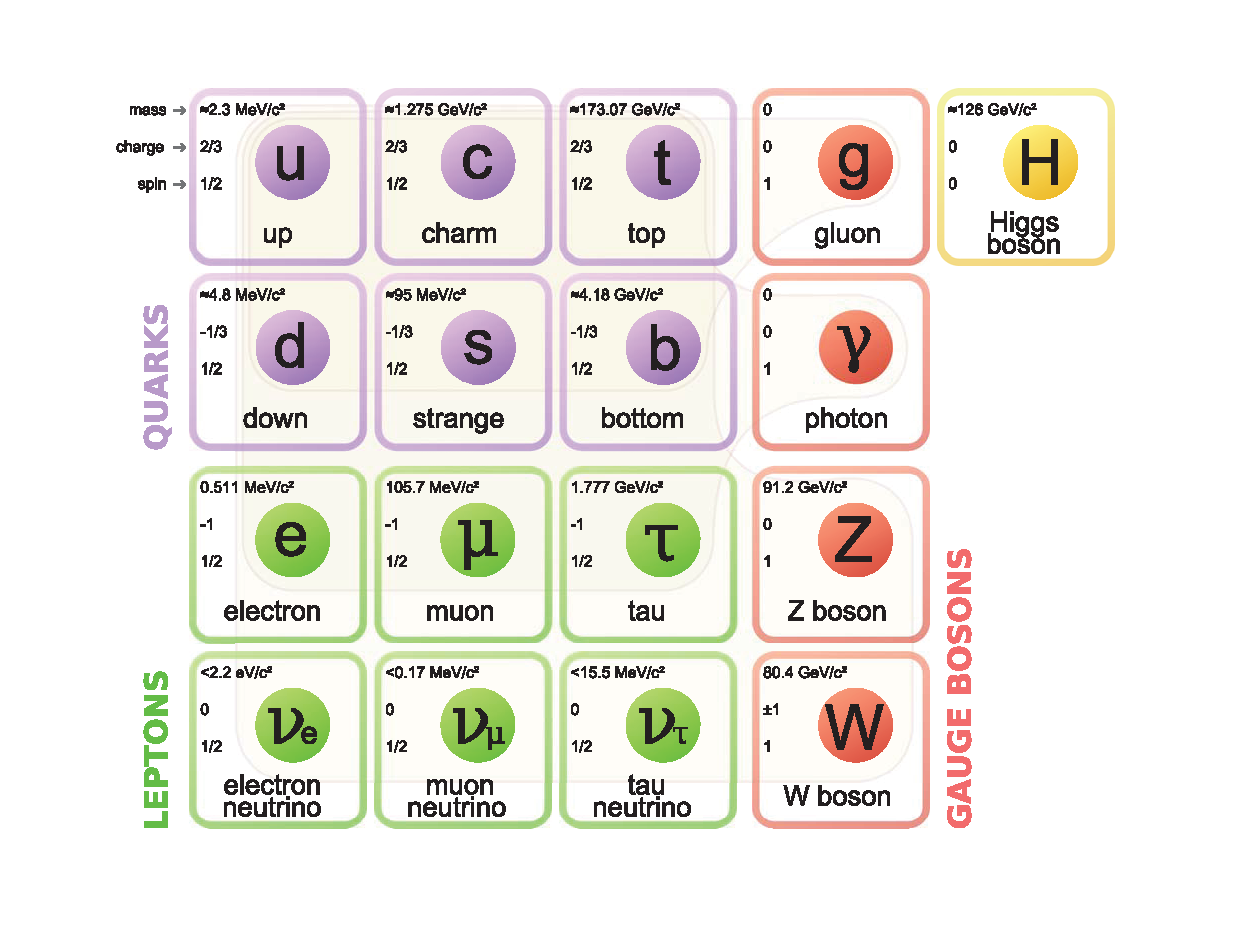
\includegraphics[width=0.8\textwidth]{chap1_SMparticles.pdf}
 \caption{粒子物理的标准模型。}
 \label{fig:SM}
\end{figure}

\begin{table}
\centering
\caption{标准模型中的三代费米子。}
%\begin{tabular*}{40cm}{llllll}
\begin{tabular}{lllll}
\toprule
&  \multicolumn{3}{c}{味道} & 电荷     \\
	\midrule
\multirow{2}*{轻子}  & $e$ & $\mu$ & $\tau$   &     -1       \\
& $\nu_{e}$ & $\nu_{\mu}$ & $\nu_{\tau}$   &     0       \\
\multirow{2}*{夸克}  & $u$ & $c$ & $t$   &     +$\frac{2}{3}$       \\
& $d$ & $s$ & $b$   &     -$\frac{1}{3}$       \\
\bottomrule
%\end{tabular*}
\end{tabular}
\label{tab:fermion}
\end{table}

\begin{table}
\centering
\footnotesize
\caption{四种玻色子及其性质。}
%\begin{tabular*}{40cm}{llllll}
\begin{tabular}{lllllll}
\toprule
名称 & 相互作用 & 自旋/宇称  & 力程(m) & 作用强度 & 典型作用时间(sec) & 理论描述  \\
	\midrule
胶子            & 强相互作用   & $1^{-}$       &  $10^{-15}$ &  1          &  $10^{-23}$  & 量子色动力学(QCD)   \\
光子            & 电磁相互作用 & $1^{-}$       &  $\infty$   &  $10^{-2}$  &  $10^{-16}$  & 量子电动力学(QED)   \\
$W^{\pm},Z^{0}$ & 弱相互作用   & $1^{-},1^{+}$ &  $10^{-18}$ &  $10^{-5}$  &  $10^{-10}$  & 量子味动力学(QFD)   \\
引力子          & 引力相互作用 & $2^{+}$       &  $\infty$   &  $10^{-39}$ &  $---$        & 广义相对论   \\
\bottomrule
%\end{tabular*}
\end{tabular}
\label{tab:SM}
\end{table}


\section{粲重子$\lambdacp$强子衰变分支比}

$\lambdacp$的质量约为质子质量的2.5倍,质量差别主要来自质子中的上夸克换成了较重的粲夸克。
粲重子$\lambdacp$作为最轻的粲重子,包含三个夸克, 即由一个重的粲夸克和两个处于同位旋$I$=0的轻夸克($u,d$)组成,如图\ref{fig:lambdac_quark}所示。
粲夸克弱衰变几乎主导了$\lambdacp$的衰变模式。
研究$\lambdacp$衰变不仅可以用来检验弱作用理论,更重要的是可以利用粲重子的跃迁来检验强相互作用机制,比如$\lambdacp$内部三个夸克的分布及相应动力学机制、以及强相互作用的SU(3)对称性等。
粲重子$\lambdacp$内部既有重夸克,又有轻夸克,因此,有其特别值得研究的地方。
这样的系统既具有重夸克对称性,又具有轻夸克手征对称性。
重夸克有效理论认为:当重夸克质量趋近无限大时,重夸克与轻夸克的自旋将退耦,重子的性质完全由轻夸克的自由度决定。
这就是通常所说的重-轻系统满足的重夸克对称性。
另外,对于较轻的$u$、$d$夸克,在取其质量为0的极限下,QCD的拉氏量具有SU(3)$_{L}$$\times$SU(3)$_{R}$的整体对称性,称为手征对称性。
研究粲重子可以很好的理解轻夸克在重夸克环境下的动力学行为, 很好的检验重夸克对称性和轻夸克手征对称性, 这对理解低能区重子和Goldstone玻色子之间的相互作用至关重要。
如图\ref{fig:charmed_baryon}所示,很多高激发态粲重子最终都要衰变到处于基态的$\lambdacp$。
不仅如此,含底夸克的$\Lambda_b$重子和$B$介子也会衰变到含$\lambdacp$末态,对$\lambdacp$衰变性质的研究也有助于进一步理解重味重子谱学及其衰变性质。
对于主要由底夸克衰变主导的实验,测量每一个底夸克产生的粲夸克数目(charm counting)以及测量唯象描述夸克强子化过程的碎裂函数,可以很好的对QCD进行检验~\cite{Abreu:1999vw,Barate:1999bg}。
而测量$\lambdacp$的强子衰变分支比对于此类问题是个重要输入量。
目前对于此类计算最大的系统误差来源已经是粲重子$\lambdacp$的衰变分支比~\cite{Dytman:2002yd,Aaij:2011jp}。

\begin{figure}[!tbp]
\begin{center}
\includegraphics[width=0.85\textwidth]{chap1_Lambda_c_quark.pdf}
\end{center}
\caption{粲重子$\lambdacp$的夸克组分示意图。}
\label{fig:lambdac_quark}
\end{figure}

\begin{figure}[!tbp]
\begin{center}
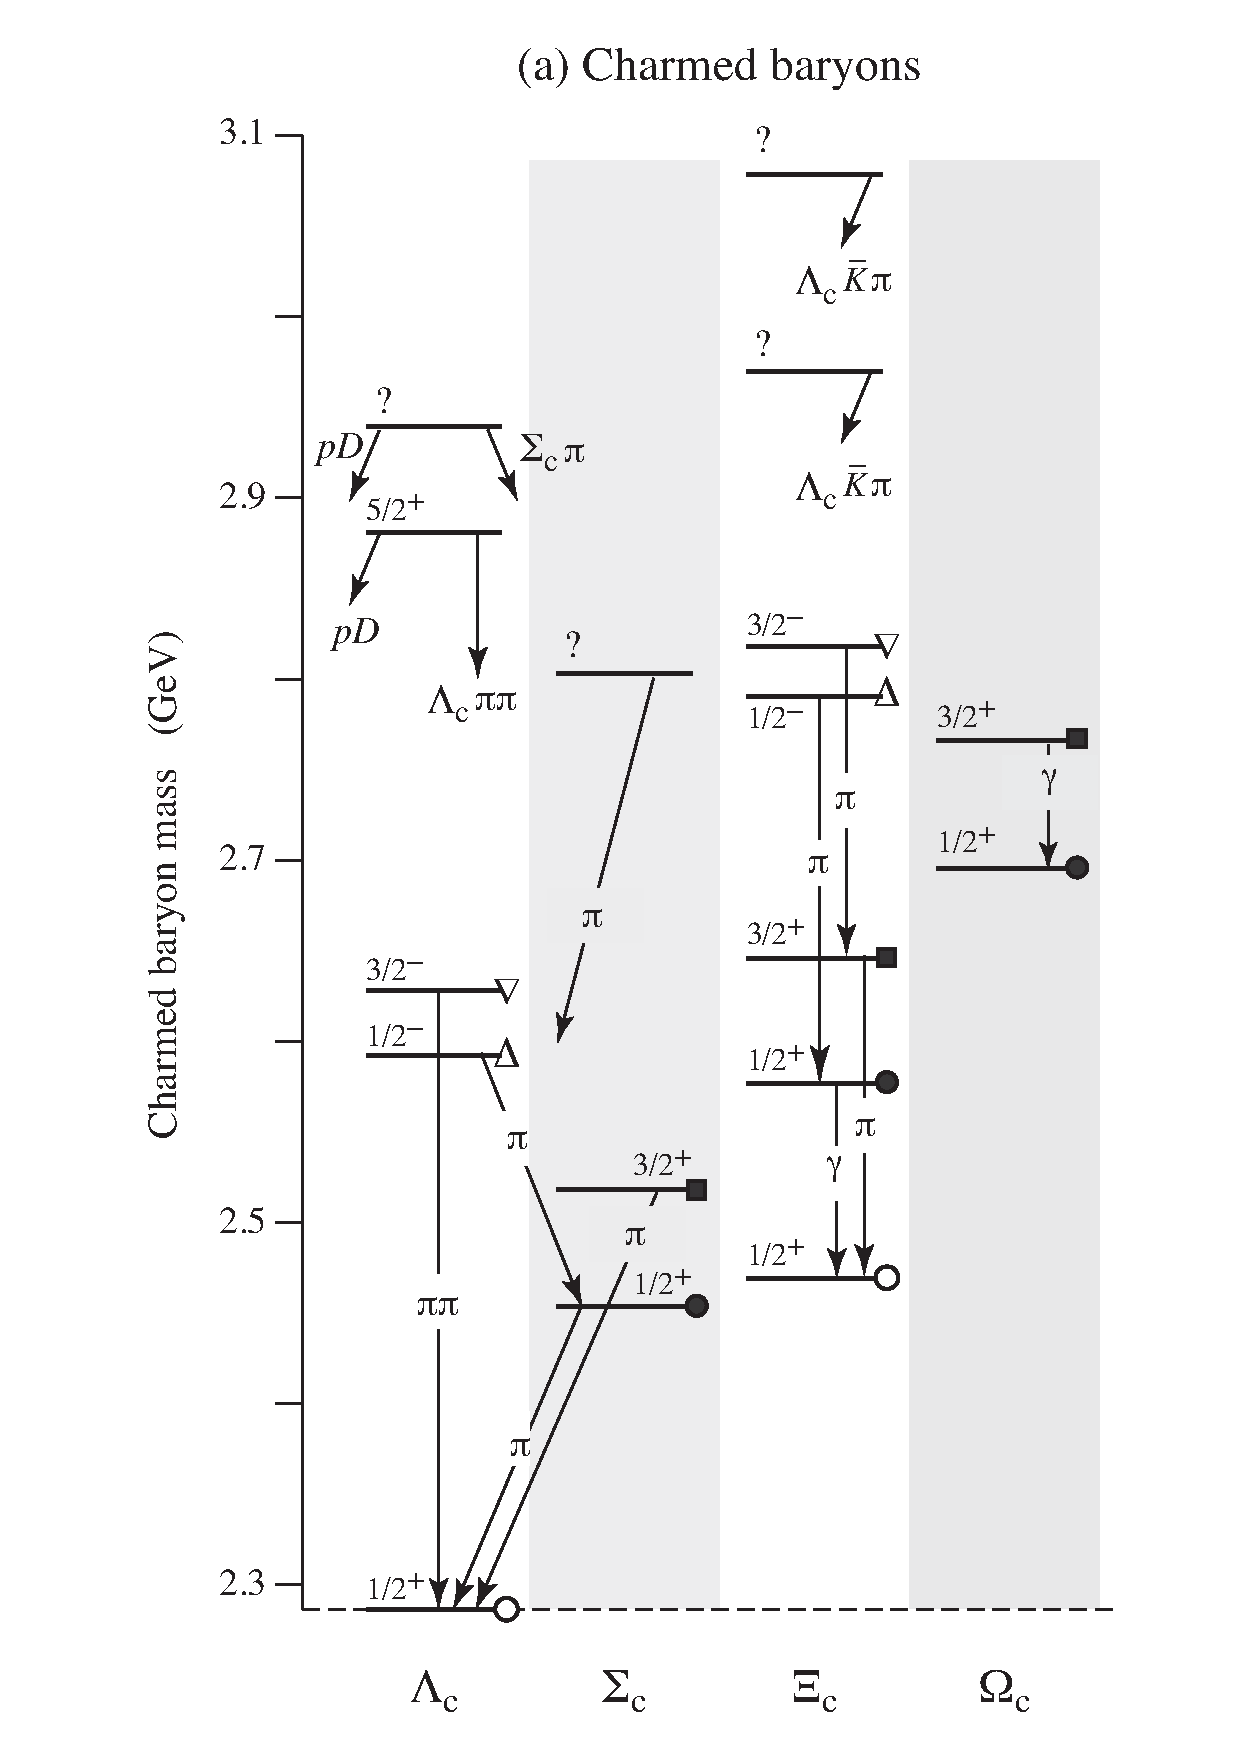
\includegraphics[width=0.85\textwidth]{chap1_charmed_baryon.pdf}
\end{center}
\caption{粲重子及其高激发态重子跃迁示意图。}
\label{fig:charmed_baryon}
\end{figure}


\subsection{$\lambdacp$ 强子衰变的相关理论现状}

描述重子结构及其性质较为成功的两个理论就是所谓的重夸克有效理论(HQET)和夸克-双夸克模型(quark-diquark)。
重夸克有效理论~\cite{Georgi:1991ch,Neubert:1993mb}是理论物理学中的一个重要工具,理由很简单:对于物理问题的理解,考虑完全的理论往往是不必要的,在一个恰当的层次上来考虑问题反而会更加行之有效。
HQET是重夸克与轻自由度直接通过软胶子交换而形成相互作用的一个简单描述。
其中重夸克的质量$m_{Q}$是一个重要的能量标度。
HQET在预言某些强子的性质时,对于重夸克质量$m_{Q}$远大于轻夸克$u,d,s$的质量情况,选择$m_{Q}\to \infty$作一个近似计算。
这时的重夸克表现的像一个色三态的静外场源,强子内动力学可以约化为轻自由度和色场源的相互作用。
然而,实际上重夸克质量并不是无限大的,尤其我们讨论的粲重子中的$c$夸克的质量并不是特别的大,因此HQET理论在这种情况下需要对除领头阶之外的其余各项做高阶修正。
重子结构的夸克-双夸克模型是Lichtenberg等~\cite{Lichtenberg:1967zz}提出的。
后来很多作者讨论过夸克-双夸克模型,虽然细节各不相同,但这些工作多少都采用了这样一个相同的物理图像。
在重子内部,有两种组分夸克和双夸克,双夸克是两个夸克的束缚态,并与第三个夸克相互作用形成重子。
对于含有两个重夸克和一个轻夸克的重子,这两个重的夸克可以组合成一个所谓的双夸克。
如果含有一个重夸克和两个轻夸克的,则这两个轻的夸克更容易形成双夸克。
双夸克模型很久以前就已经被很多理论的文章采用,计算了很多涉及重子的过程~\cite{Anselmino:1987vk, Kroll:1987pj,Mannel:1990vg,Leinweber:1993nr,Ebert:1995fp}。
它有着明显的优点,化三体问题为两体问题,使计算大为简化。
用这一模型讨论重子介子散射、重子磁矩以及定性地讨论重子质量方面取得了一些成功。


具体到理论方面的计算。
介子和重子所有的非轻子衰变都可以归为如下几类的拓扑图: W外发射,W内发射,W交换图,W湮灭图和W圈图。
图\ref{fig:feynman_lambdapip}给出了粲重子$\lambdacp\to \Lambda \pip$衰变过程的三种典型拓扑图(W外发射,W内发射和W交换),其它衰变过程的图像大多与此类似的。
粲重子$\lambdacp$的衰变中是没有湮灭图贡献的。
我们研究的Cabibbo 允许的过程也不会出现圈图的贡献。
对于W内发射和外发射图通常认为是可因子化部分~\footnote{ W内发射意味着W出来的两个夸克要和其余夸克进行强子化,因此会有所谓的色压低效应。},而对于W交换和W湮灭图是不可以因子化的。
粲重子中的W内发射对可因子化提出了更高的要求,即通过弱衰变来的夸克要强子化成介子的情形才可以因子化,而强子化成重子的过程是不可以因子化的。
图\ref{fig:feynman_pK0bar}给出了粲重子$\lambdacp\to p \overline{K}{}^{0}$衰变过程的两个可能拓扑图(W内发射和W交换)。
我们可以清楚的看到图\ref{fig:feynman_lambdapip_C}中$s$夸克出现在重子$\Lambda$中,故该拓扑图是不可因子化的,而图\ref{fig:feynman_pK0bar_C}中$s$夸克是出现在介子$\overline{K}{}^{0}$中,故可以简单地认为该图是可以因子化的(后面会看到也有不可因子化的贡献)。

\begin{figure}[!tbp]
 \centering
\subfigure[W外发射T图]
{
 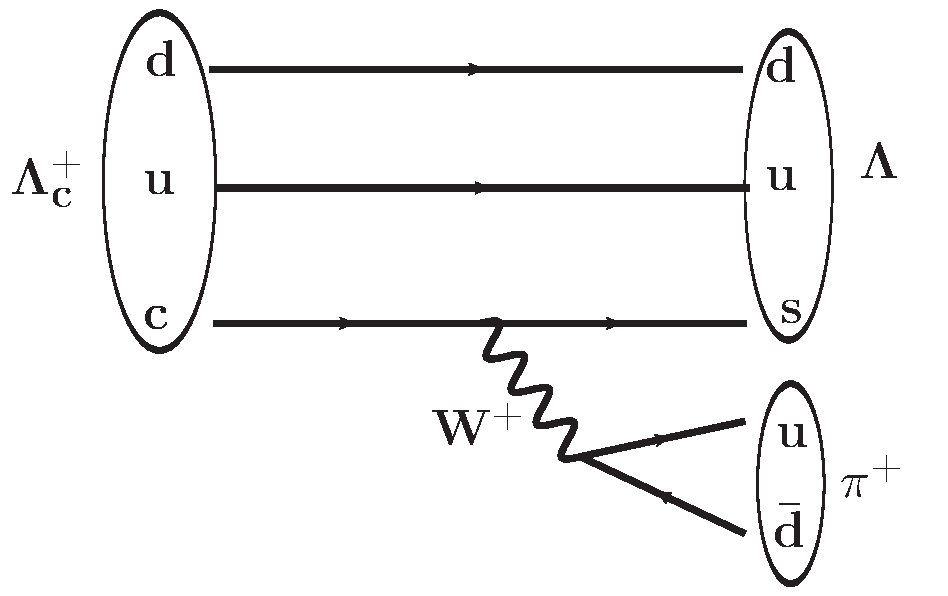
\includegraphics[width=0.3\textwidth]{chap1_feynman_lambdapi_external.pdf}
 \label{fig:feynman_lambdapip_T}
}
\subfigure[W内发射C图]
{
 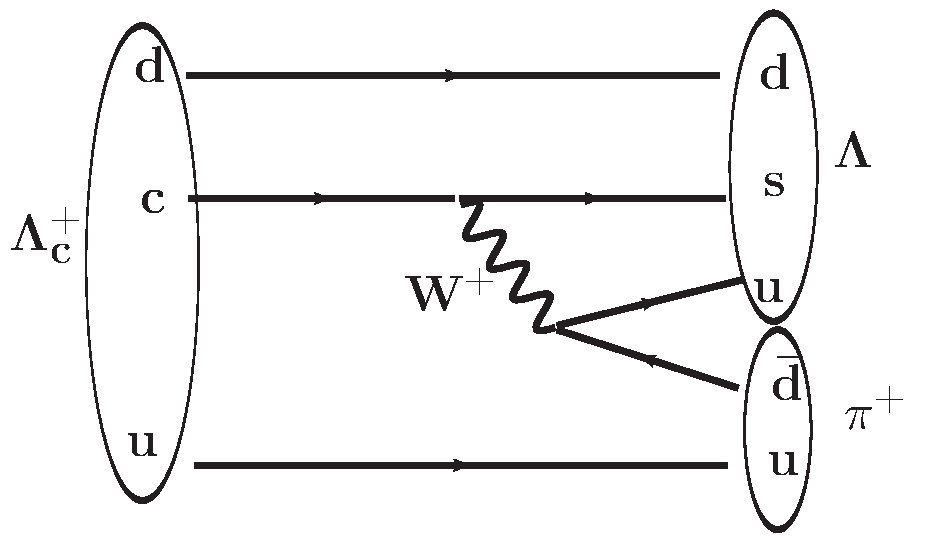
\includegraphics[width=0.3\textwidth]{chap1_feynman_lambdapi_internal.pdf}
 \label{fig:feynman_lambdapip_C}
}
\subfigure[W交换E图]
{
 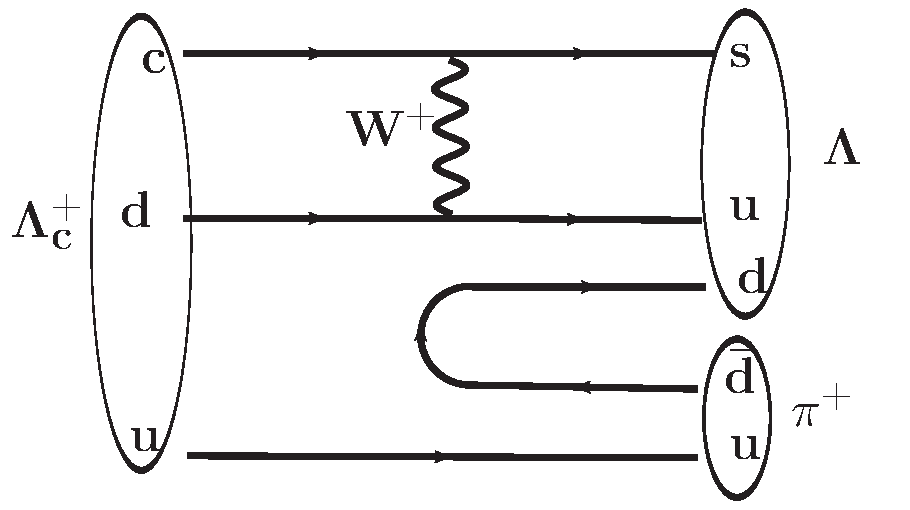
\includegraphics[width=0.3\textwidth]{chap1_feynman_lambdapi_exchange.pdf}
}
 \caption{粲重子$\lambdacp \to \Lambda\pip$衰变的典型拓扑图。}
 \label{fig:feynman_lambdapip}
\end{figure}

\begin{figure}[!tbp]
 \centering
\subfigure[W内发射C图]
{
 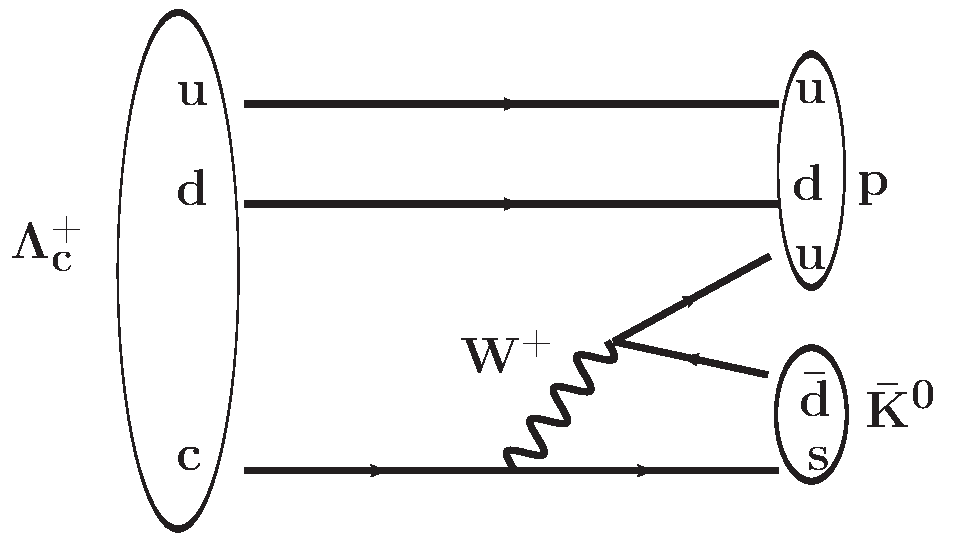
\includegraphics[width=0.4\textwidth]{chap1_feynman_pK0bar_internal.pdf}
 \label{fig:feynman_pK0bar_C}
}
\subfigure[W交换E图]
{
 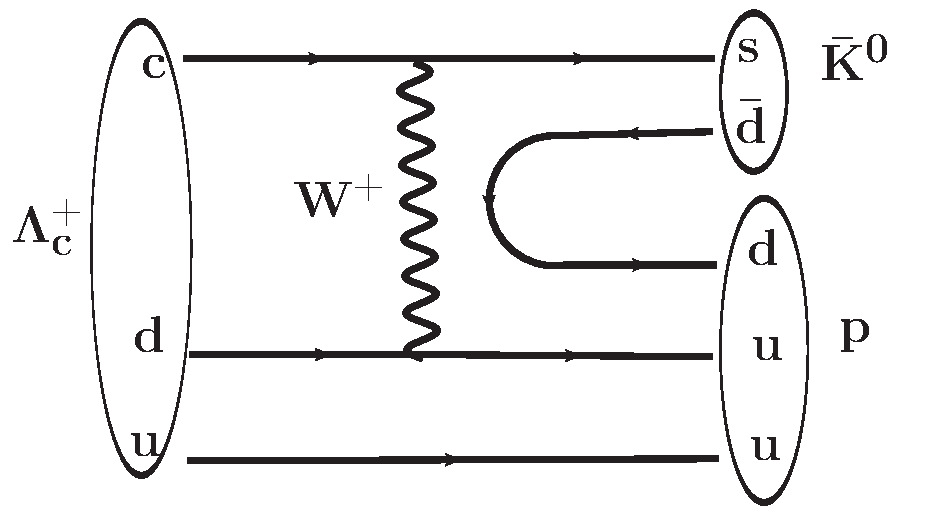
\includegraphics[width=0.4\textwidth]{chap1_feynman_pK0bar_exchange.pdf}
}
 \caption{粲重子$\lambdacp \to p \overline{K}{}^{0}$衰变的典型拓扑图。}
 \label{fig:feynman_pK0bar}
\end{figure}

%由于理论上对于粲重子的计算还非常有限,我们尝试对应粲介子中的计算情况对粲重子的对应情况先进行一个相应的讨论:
众所周知,粲介子中不可因子化的W交换过程存在着色压低和螺旋度压低,与可因子化的发射图贡献相比,可因子化部分是占主导地位的。
简单因子化方法将外发射(图\ref{fig:feynman_lambdapip_T})和内发射(图\ref{fig:feynman_pK0bar_C},区别于图\ref{fig:feynman_lambdapip_C})贡献$a_{1}$,$a_{2}$分别写为~\cite{Fusheng:2011tw,Li:2012cfa}:
\begin{equation}
a_1(\mu)=C_2(\mu)+\frac{C_1(\mu)}{N_c},
a_2(\mu)=C_1(\mu)+\frac{C_2(\mu)}{N_c},
\end{equation}
$C_{1,2}$称作威尔逊系数,可以通过微扰论进行计算,$N_{c}$在因子化方法中指的是颜色的数目3。
其中$\mu=\sqrt{\Lambda m_D (1-r_1^2)(1-r_2^2)}$为威尔逊系数能标,$r_{1,2}$为与初末态相关的质量比值。
$\Lambda$与末态粒子在D介子中的动量有关。
粲介子环境下典型的能标$\mu\sim 1\gev$。
我们通过粲介子的衰变研究已经知道简单因子化方法描述色压低过程是不完备的,需要引入所谓的大$N_{c}$方法~\cite{Buras:1985xv}。
大$N_{c}$方法的核心就是通过修正W内发射的振幅$a_{2}$~中~$N_{c}$这一项,来唯象的描述色压低的效应。
大$N_{c}$方法在粲介子计算中的应用显著改善了实验和理论的一致性~\cite{Fukugita:1977df,Tadic:1982vn,Bauer:1984zv}。
这一结论也得到了QCD求和规则方法的验证~\cite{Blok:1986um,Blok:1986hm,Blok:1986sn}。
另一种有效解决简单因子化方法描述色压低过程不够好的方法是引入新的一项$\chi_{nf} e^{i\phi}$来描述不可因子化的部分~\cite{Fusheng:2011tw,Li:2012cfa}。
同时忽略外发射图的不可因子化贡献,则新的能标依赖的威尔逊系数可以写为
\begin{eqnarray}
\label{effa}
a_1^{\mu}=C_2(\mu)+\frac{C_1(\mu)}{N_c},
a_2^{\mu}=C_1(\mu)+C_2(\mu)\bigg(\frac{1}{N_c}+\chi_{nf} e^{i\phi}\bigg),
\end{eqnarray}
式中参数$\chi_{nf}$~和~$\phi$为新引入的参数用以描述图\ref{fig:feynman_pK0bar_C}这一类拓扑图中的不可因子化部分。
这些参数对于不同的衰变道应该是公用的,其具体的数值只能通过实验数据来确定。
显然地,当$\chi_{nf} e^{i\phi}=-1/N_c$的时候两种方法是等效的。
同时也应注意到大$N_{c}$方法实际上没有考虑$a_1^{\mu}$和$a_2^{\mu}$这两部分之间存在着的强相角。
而实验数据告诉我们$a_1^{\mu}$和$a_2^{\mu}$这两部分贡献之间的相角往往很大。
为了理论计算方便往往认为$a_1$为实的,把相角归为$a_2$内,即
\begin{eqnarray}
a_1=|a_1|,&& a_2=|a_2|e^{i\delta},
\end{eqnarray}


很自然地,理论学家尝试将其应用到粲重子的计算过程中去。
但是这种方式对于粲重子是否适用还需要检验,理论学家找到了一个特殊的~Cabibbo~压低的衰变道$\Lambda_c^+\to p\phi$去计算以和实验进行对比。
如图~\ref{fig:feynman_pphi}所示, 这个过程只有内发射图的贡献是主导的,属于典型的图\ref{fig:feynman_pK0bar_C}类似的情况,也没有外发射的图来产生干涉效果,可以拿来很好的来验证粲重子中上述大$N_{c}$方法是否适用。
\begin{figure*}[!tbp]
\centering
\subfigure[]
{
 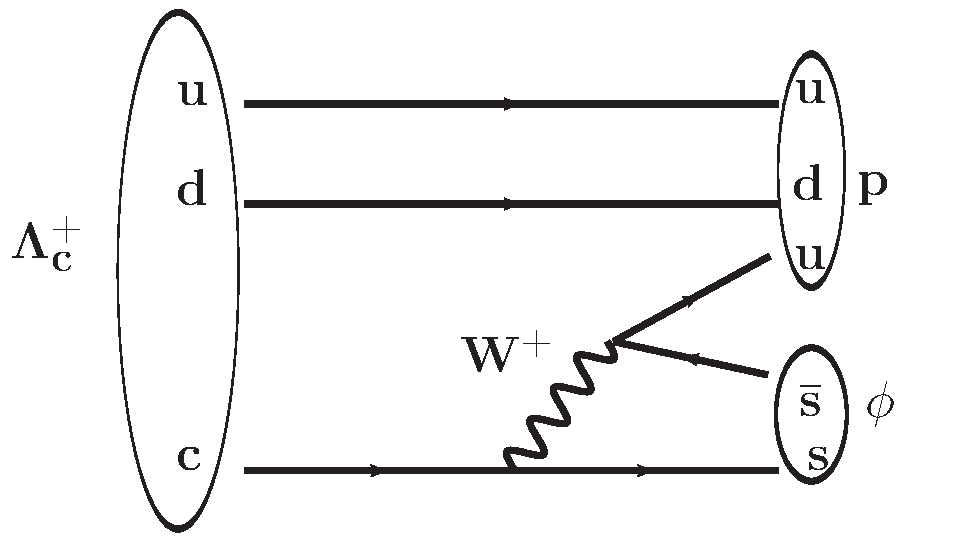
\includegraphics[width=0.4\textwidth]{chap1_feynman_pphi.pdf}
}
 \caption{$\lambdacp\to p\phi$过程W内发射拓扑图。}
\label{fig:feynman_pphi}
\end{figure*}
文献~\cite{Cheng:1991sn}指出了大$N_{c}$方法计算出的$\Lambda_c^+\to p\phi$衰变分支比和实验测量是一致的。
如果只用简单因子化方法计算,结果与实验测量值小了约15倍,这很好的说明了该方法同样适用于粲重子中的类似情形。

虽然如此,在粲重子还是有着其独特的情况的。不可因子化的W交换过程在粲重子中不再是色压低和螺旋度压低的。
不可因子化的作用与可因子化部分相比并不低甚至比可因子化部分更主导。
理论上对于粲重子的分支比计算过程中不确定性最大的就是在于如何处理不可因子化的W交换过程上。
历史上比较有名的的模型是流代数模型,1992年之前一直在广泛使用~\cite{Cheng:1993gf}。
然而它也有着其局限性:要求两体衰变过程中的介子一定是赝标量介子,且一定要足够软。
这一要求往往是不被满足的。
所以理论学家不得不转向了更基本的极点模型(pole model)。
其简单的图像就是将粲重子中不可因子化部分的贡献近似为一个中间共振态粒子的动力学行为。
文献~\cite{Asner:2008nq}给我们总结了各个模型计算出粲重子强衰变的分支比计算结果。
目前理论上可以计算的只有两体过程。
这些模型大都是利用的极点模型来计算的结果,只不过在处理非可因子化部分的细节上存在着差异。
文献~\cite{Sharma:1998rd}更加注重处理W交换过程在强衰变里面的作用,
通过对比我们发现随着理论的发展其结果与实验变得越来越一致。
这再一次启示我们在粲重子衰变中不可因子化的W交换过程起着非常主要的角色。

如图~\ref{fig:feyman_xik}所示,$\Lambda^+_c\to \Xi^{(*)0}K^+$过程只能通过图示W交换过程才能发生的,
同时,此一过程,在$S$波和$P$波的衰变振幅中均存在着不同强子衰变矩阵元之间的大幅相消,从而导致此过程的理论计算非常困难,且具有非常大的不确定性,如表~\ref{tab:prediction}所示。
理论预言给出的$\mathcal{B}(\Lambda^+_c\to\Xi^{0}K^+)$ 落在$[1.0, 3.6] \times 10^{-3}$~\cite{Korner:1992wi,Zenczykowski:1993hw,Ivanov:1997ra, Xu:1992vc,Sharma:1998rd}区间之内,
而对于$\mathcal{B}(\Lambda^+_c\to\Xi^{*0}K^+)$,给出的三个理论计算结果更是有量级上的差异~\cite{Korner:1992wi,Xu:1992sw,Fayyazuddin:1996iy}。
我们去寻找和测量此一过程对于理解粲重子中不可因子化贡献起到非常重要的作用。
测定此类过程的分支比对于理论来说是个重要的检验,同时也是一个重要的输入。

%%%%%%%%%%%%
\begin{figure}[!tbp]
\begin{center}
	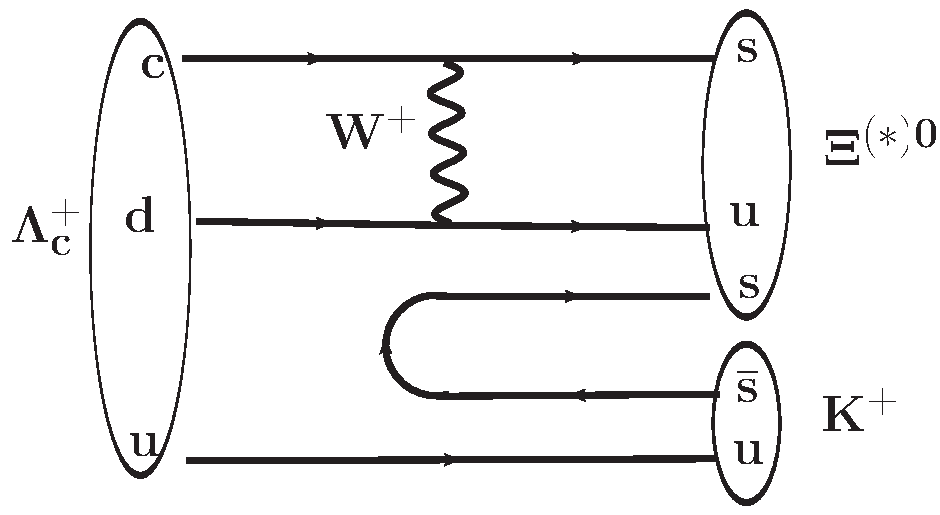
\includegraphics[width=0.45\linewidth]{chap1_feynman_XiK_exchange1.pdf}
	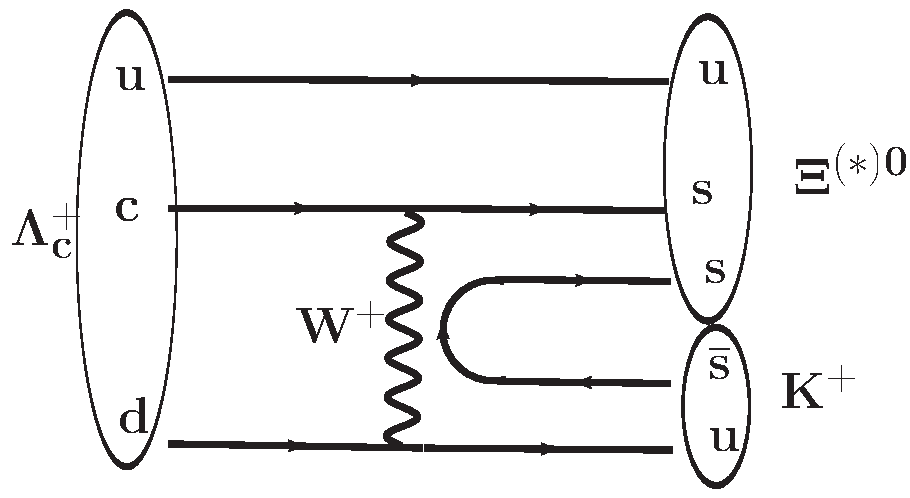
\includegraphics[width=0.45\linewidth]{chap1_feynman_XiK_exchange2.pdf}
\caption{ $\LtoXiXisK$ 过程W交换拓扑图。}
\label{fig:feyman_xik}
\end{center}
\end{figure}
%%%%%%%%%%%%

\begin{table}[H]
\caption{$\mathcal{B}(\LtoXiXisK)$的实验测量值与理论预言值比较。}
\begin{center}
  \resizebox{\linewidth}{!}{
\begin{tabular}{l|c|c|c}
\hline\hline
\multirow{2}*{\minitab[c]{衰变道\\ }}                       &  \multirow{2}*{\minitab[c]{其它实验的测量 $\frac{\mathcal{B}(\Lambda^+_c\to\Xi^{(*)0}K^+)}{\mathcal{B}(\Lambda^+_c\to p K^- \pi^+)}$ \\ }}   & \multirow{2}*{\minitab[c]{PDG报道 \\ $\mathcal{B}(\Lambda^+_c\to\Xi^{(*)0}K^+)$ \\ }}  & \multirow{2}*{\minitab[c]{理论预言 \\ $\mathcal{B}(\Lambda^+_c\to\Xi^{(*)0}K^+)$\\ }}  \\
                            &                   &                                 &     \\ \hline
\multirow{5}{*}{$\XiK$}     &  \multirow{5}*{\minitab[c]{$(7.8\pm 1.8)\%$~\cite{Avery:1993vj} \\ }}  &    \multirow{5}*{\minitab[c]{$(5.0\pm 1.2)\times10^{-3}$~\cite{PDG2017} \\ }}  &  2.6$\times10^{-3}$~\cite{Korner:1992wi}  \\
                            &                   &                                 &  3.6$\times10^{-3}$~\cite{Zenczykowski:1993hw}  \\
                            &                   &                                 &  3.1$\times10^{-3}$~\cite{Ivanov:1997ra}  \\
                            &                   &                                 &  1.0$\times10^{-3}$~\cite{Xu:1992vc}  \\
                            &                   &                                 &  1.3$\times10^{-3}$~\cite{Sharma:1998rd}  \\ \hline
\multirow{3}{*}{$\XisK$}    &   \multirow{3}*{\minitab[c]{$(5.3\pm1.9)\%$~\cite{Avery:1993vj}  \\ $(9.3\pm3.2)\%$~\cite{Albrecht:1994hr} }} & \multirow{3}*{\minitab[c]{$(4.0\pm 1.0)\times10^{-3}$~\cite{PDG2017} \\ }}  & \multirow{3}*{\minitab[c]{5.0$\times10^{-3}$~\cite{Korner:1992wi}  \\  0.8$\times10^{-3}$~\cite{Xu:1992sw}  \\  0.6$\times10^{-3}$~\cite{Fayyazuddin:1996iy} }} \\
                            &                   &                                 &     \\ 
                            &                   &                                 &     \\ \hline \hline
\end{tabular}
}
\label{tab:prediction}
\end{center}
\end{table}




\subsection{实验现状}

实验上多数关于$\lambdacp$的研究是20多年前开展的,主要以$\Lmodeb$衰变作为参考道来研究强子衰变的分支比。
然而对于$\Lmodeb$分支比的实验测量并不准确,都或多或少地依赖于模型假设。
这从整体上使$\Lmodeb$衰变分支比的结果存在很大的不确定性。
过去的20年间,粲介子的研究取得了长足的发展。相反的是,在重子谱研究尤其是粲重子谱研究方面进展相对缓慢。主要原因还是因为缺乏有效的实验数据。 
表~\ref{tab:compare_meason_baryon}给出了粲介子和粲重子典型衰变道的测量精度比较。很容易我们可以发现粲重子的精度比粲介子的精度差很多。
\begin{table}
\centering
\footnotesize
\caption{PDG2014中粲强子典型衰变道的实验精度比较。}
\begin{tabular}{l|cc|cc}
%\toprule
 \hline \hline
粲强子 & 强子衰变道 & 精度($\delta \mathcal{B}/\mathcal{B}$)  & 半轻衰变道 & 精度($\delta \mathcal{B}/\mathcal{B}$) \\
%	\midrule
 \hline
$\Dz$     &  $\mathcal{B}(K^{-}\pi^{+})=(3.88\pm0.05)\%$         &  $1.3\%$ &  $\mathcal{B}(K^{-}e^{+}\nu_{e})=(3.55\pm0.05)\%$   &  $1.4\%$  \\
$\Dp$     &  $\mathcal{B}(K^{-}\pi^{+}\pi^{+})=(9.13\pm0.19)\%$  &  $2.1\%$ &  $\mathcal{B}(K^{0}e^{+}\nu_{e})=(8.83\pm0.22)\%$   &  $2.5\%$  \\
$D_{s}^{+}$  &  $\mathcal{B}(K^{+}K^{-}\pi^{+})=(5.39\pm0.21)\%$    &  $3.9\%$ &  $\mathcal{B}(\phi e^{+}\nu_{e})=(2.49\pm0.14)\%$   &  $5.6\%$  \\
 \hline
$\lambdacp$  &  $\mathcal{B}(pK^{-}\pi^{+})=(5.0\pm1.3)\%$          &  $26\%$  &  $\mathcal{B}(\Lambda e^{+}\nu_{e})=(2.1\pm0.6)\%$  &  $29\%$   \\
 \hline \hline
%\bottomrule
\end{tabular}
\label{tab:compare_meason_baryon}
\end{table}
图~\ref{fig:br_lambdac_pdg}是PDG2014中$\lambdacp$各个衰变分支比的大小示意图。其中很多道的分支比结果都是采用的$\mathcal{B}(pK^{-}\pi^{+})=(5.0\pm1.3)\%$来进一步计算的(之前的实验大多都是相对$pK^{-}\pi^{+}$的测量)。
\begin{figure}[!tbp]
 \centering
\subfigure[$\mathcal{B}(pK^{-}\pi^{+})$采用PDG2014中的结果。]
{
 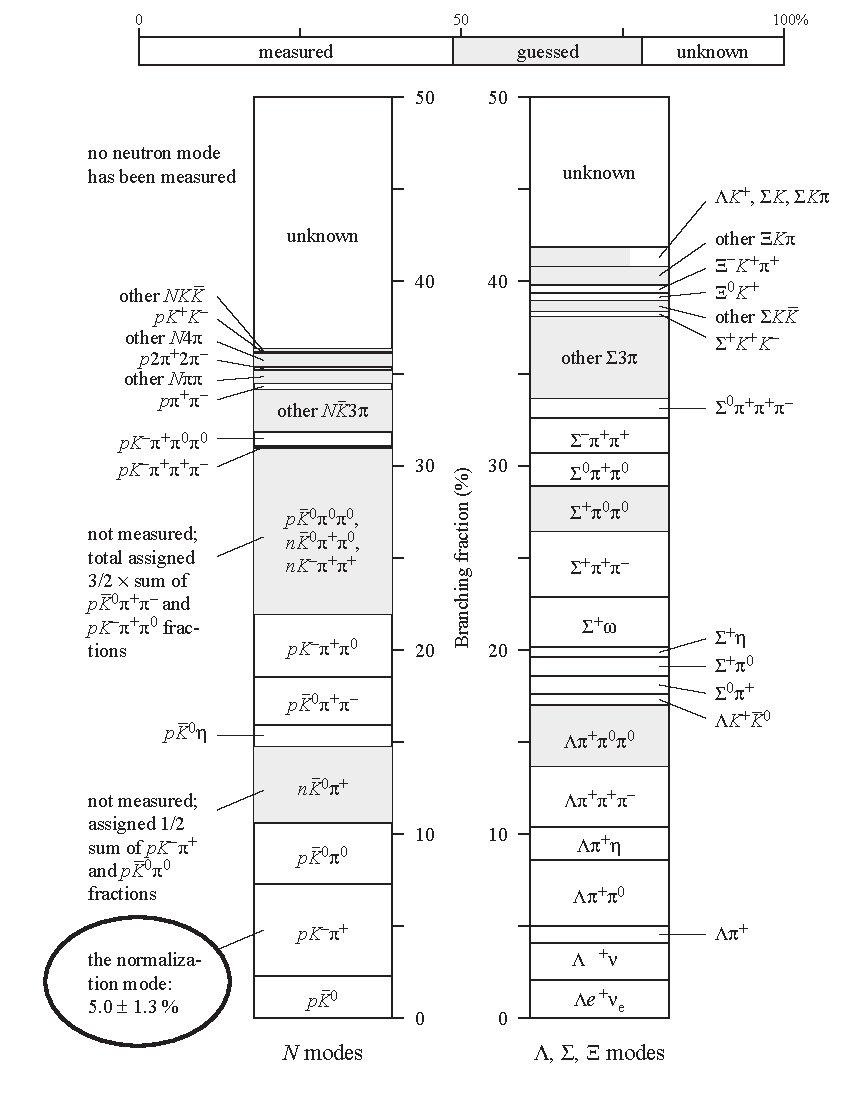
\includegraphics[width=0.45\textwidth]{chap1_br_lambda_c_1.pdf}
 \label{fig:br_lambdac_pdg}
}
\hspace{1pt}
\subfigure[$\mathcal{B}(pK^{-}\pi^{+})$采用Belle测量的结果。]
{
 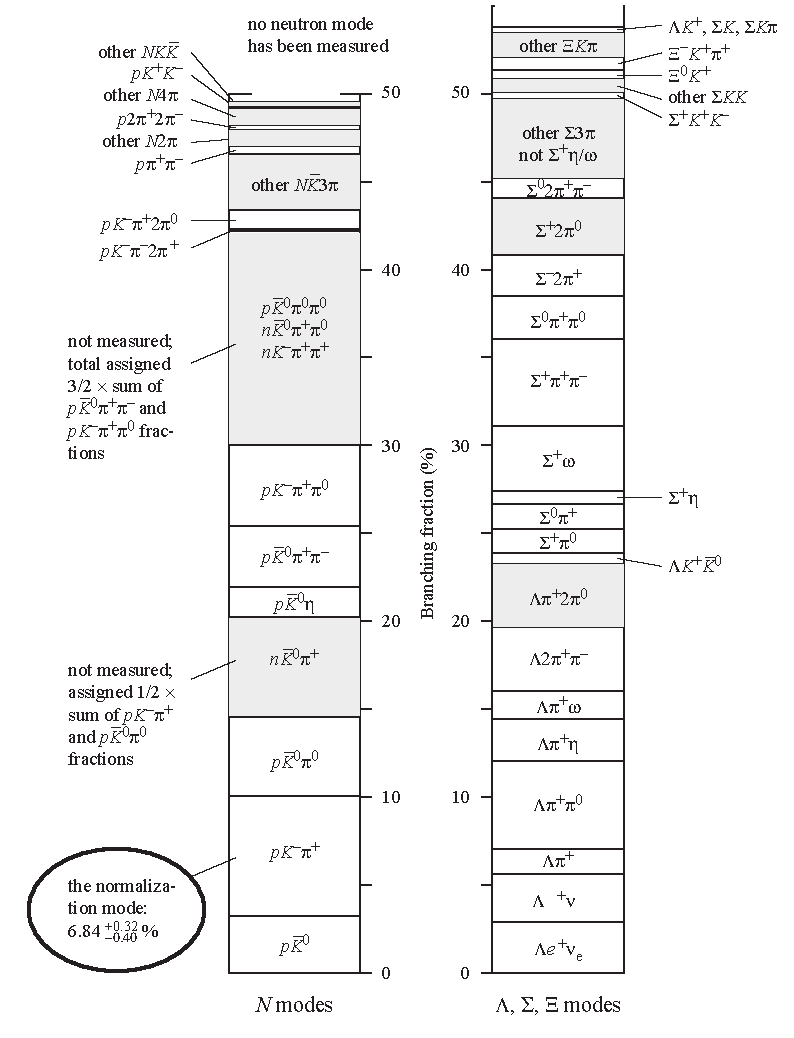
\includegraphics[width=0.45\textwidth]{chap1_br_lambda_c_2.pdf}
 \label{fig:br_lambdac_belle}
}
 \caption{粲重子$\lambdacp$已测量(measured)和未测量(guessed和unknown)衰变分支比大小示意图。}
 \label{fig:br_lambdac}
\end{figure}
从图中我们可以清楚的看到有很多的衰变道没有很好的测量,尤其是末态含有中子的衰变道,基本都是理论预测的结果。
同时我们也注意到这些已知的所有的$\lambdacp$的衰变道的总的分支比远小于1。
这也在一定程度上说明当前的$\mathcal{B}(pK^{-}\pi^{+})$的结果有可能偏低。

Belle实验利用他们在$\Upsilon(nS)$上采取的数据,采用初态辐射的技术在2014年报道了他们测量的$\Lmodeb$的衰变分支比结果$\br{\modeb}=(6.84\pm0.24^{+0.21}_{-0.27})\%$~\cite{Lambdac_belle}。
测量结果的精度达到了$4.7\%$,较PDG2014好了有5倍之多。
这一结果是首次进行的绝对测量, 测量也是模型无关的。
但是我们从图~\ref{fig:bellepaper}~\cite{Lambdac_belle}可以注意到,Belle实验的拟合结果遭受着高本底的污染,这主要是由于其运行在高能量区域所导致的。
\begin{figure}[!tbp]
 \centering
 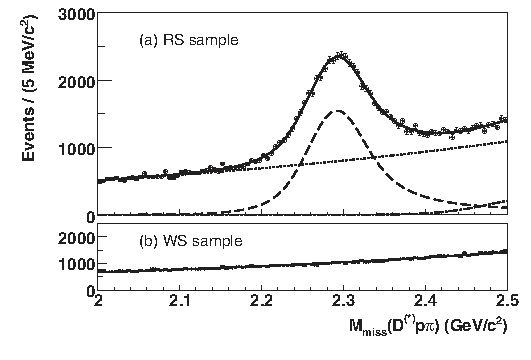
\includegraphics[width=0.8\textwidth]{chap1_belle_paper.pdf}
 \caption[Belle实验的拟合结果图。]{Belle实验的拟合结果图,摘选自文献~\cite{Lambdac_belle}。}
 \label{fig:bellepaper}
\end{figure}
除此之外,高端还遭受着高激发态本底的尾巴的影响,这会大大增加信号数获取的不准确度。
图~\ref{fig:br_lambdac_belle}是采用了Belle的结果$\mathcal{B}(pK^{-}\pi^{+})=(6.84\pm0.24^{+0.21}_{-0.27})\%$来进一步计算之后的$\lambdacp$各个衰变分支比的大小示意图。
我们注意到这些已知的所有的$\lambdacp$的衰变道的总的分支比之和已经超过100\%了。
如果说之前的相对测量是准确的话,那么这在一定程度上暗示Belle的$\mathcal{B}(pK^{-}\pi^{+})$的结果有可能偏高。
BESIII在2016年的时候测量了$\mathcal{B}(pK^{-}\pi^{+})=(5.84\pm0.27\pm0.23)\%$~\cite{Lambdac_bes3},当PDG2016~\cite{PDG2017}合并了BESIII和Belle的结果之后给出$\mathcal{B}(pK^{-}\pi^{+})=(6.35\pm0.33)\%$,从而缓解了Belle测量结果导致分支比超出的问题。


实验上,$\cleo$~\cite{Avery:1993vj}合作组和$\argus$~\cite{Albrecht:1994hr}合作组对于$\Lambda^+_c\to \Xi^{(*)0}K^+$衰变分支比进行过一些测量。
不过这些测量都是20多年前进行的,而且它们都是相对于$\mathcal{B}(\Lmodeb)$的相对测量。它们的测量结果我们同样展示在表~\ref{tab:prediction}中以进行比较。
PDG2016中关于此两个衰变道的结果分别为$\mathcal{B}(\Lambda^+_c\to\Xi^0K^+)=(5.0\pm1.2)\times10^{-3}$~\cite{PDG2017} 和 $\mathcal{B}(\Lambda^+_c\to\Xi^{*0}K^+)=(4.0\pm1.0)\times10^{-3}$~\cite{PDG2017}~\footnote{假定$\Xi(1530)^0\to\Xi^{-}\pi^{+}$的分支比为$\frac{2}{3}$,用它来修正文献~\cite{Albrecht:1994hr}中$\argus$的测量值。}。
BESIII实验利用阈值上的$\ee$湮灭数据去研究$\lambdacp$衰变是更简单更直接的一种方式,这种方式有着其独特的优势所在。
在阈值上$\Lambda_c$是成对产生的,除了$\Lambda_c$对之外不会有额外的任何强子产生。
这就给我们提供了一个非常干净的$\Lambda_c$的产生环境。
此外,由于是成对产生,我们可以双标记的技术来进行测量。
这样一来,双标记侧几乎是没有本底的,结果更加可靠。
另外一个就是双标记方法可以做到绝对测量,单标记的系统误差基本可以认为消除掉了。这也是阈值上数据的优势。
基于BESIII在 $\sqrt{s}=4.6\gev$ 处采集的567\,pb$^{-1}$的$\ee$对撞数据,运用成熟的双$\Lambda_{c}$标记技术我们可以对$\mathcal{B}(\Lambda^+_c\to \Xi^{(*)0}K^+)$进行首次的绝对测量。

\section{重夸克偶素产生的研究现状}
\subsection{重夸克偶素简介}

重夸克是指粲夸克($c$)、底夸克($b$)和顶夸克($t$),他们都比较重,尤其是顶夸克$t$特别的重,寿命在$10^{-13}$量级上,几乎来不及形成强子。
重夸克偶素~\cite{Lansberg:2008gk}是指带有各种$J^{PC}$ 量子数的$c\bar{c}$和$b\bar{b}$ 束缚态,其中$J^{PC}$由两个组合重夸克的总自旋S和总角动量L决定。
重夸克偶素的物理过程涉及了QCD的所有能区。
在高能区偶合常数是可适用的,QCD 微扰展开易于收敛;而到了低能区域,非微扰是主导的,QCD失效了,只能通过其他非微扰方法来处理~\cite{Kramer:2001hh}。
重夸克偶素物理过程的研究对考察微扰与非微扰QCD交叠区域的动力学,检验和发展QCD 模型起着重要意义。
在过去的三十多年里,许多理论工作也验证了QCD在重夸克偶素上的应用。
历史上比较流行的理论基本上有三种:色单态机制(CSM)、 色蒸发模型 (CEM)、 色八重态机制(COM)。
伴随着实验的进程,人类已经提前对QCD有了一个很好的理解。
理论计算和实验都在夸克偶素的产生上做出了很大的贡献,然而还存在着很多问题~\cite{Brambilla:2010cs}。
例如,色单态模型在解释Tevatron上正反质子对撞实验中高横动量$\pt$下$\jpsi$ 粒子的产生截面时遇到了很大的困难,产生了数量级上的差异。
COM应用了1986 年被Caswell 和Lapage 发展起来的有效场论发展出了非相对论量子色动力学(Non-Relativistic QCD,NRQCD),
目前成为主流的描述强产生的里面模型,在高$\pt$区域描述的比较好。
虽然NRQCD能够很好地解释实验上测得的重味夸克偶素的产生截面,但极化预测值与CDF 实验所测结果相矛盾~\cite{Lansberg:2008gk}。
COM 和领头阶(LO) CSM理论,预言了高横动量下重夸克偶素的极化,但是不能解释强子对撞中$\psi(nS)$ 和$\Upsilon(nS)$ 的极化。
基于非微扰QCD框架开发的Fixed-Order-with-Next-to-Leading-Logarithm (FONLL)~\cite{Cacciari:1998it}成功的用于描述多个非直接产生的重夸克偶素态的产生截面。

\subsection{$\lhcb$上重夸克偶素的研究}

大型强子对撞机$\lhc$上,在质子质子对撞为2.76$\tev$,7$\tev$,8$\tev$和13$\tev$的质心系能量下,$\atlas$、$\cms$、$\alice$ 和$\lhcb$四个实验都对夸克偶素进行过研究。
我们接下来以$\lhcb$实验上$\jpsi$和$\psitwos$在7$\tev$质心系能量下为例介绍目前对重夸克偶素的产生截面测量以及极化测量情况。

在高能对撞实验上,以粲夸克偶素为例(图\ref{fig:charmonium} 给出了按照$J^{PC}$和质量总结的各个粲偶素和类粲偶素粒子),其产生主要有三种来源:部分子碰撞直接产生,高激发态退激发产生以及$b$强子衰变产生。
\begin{figure}[!tbp]
\begin{center}
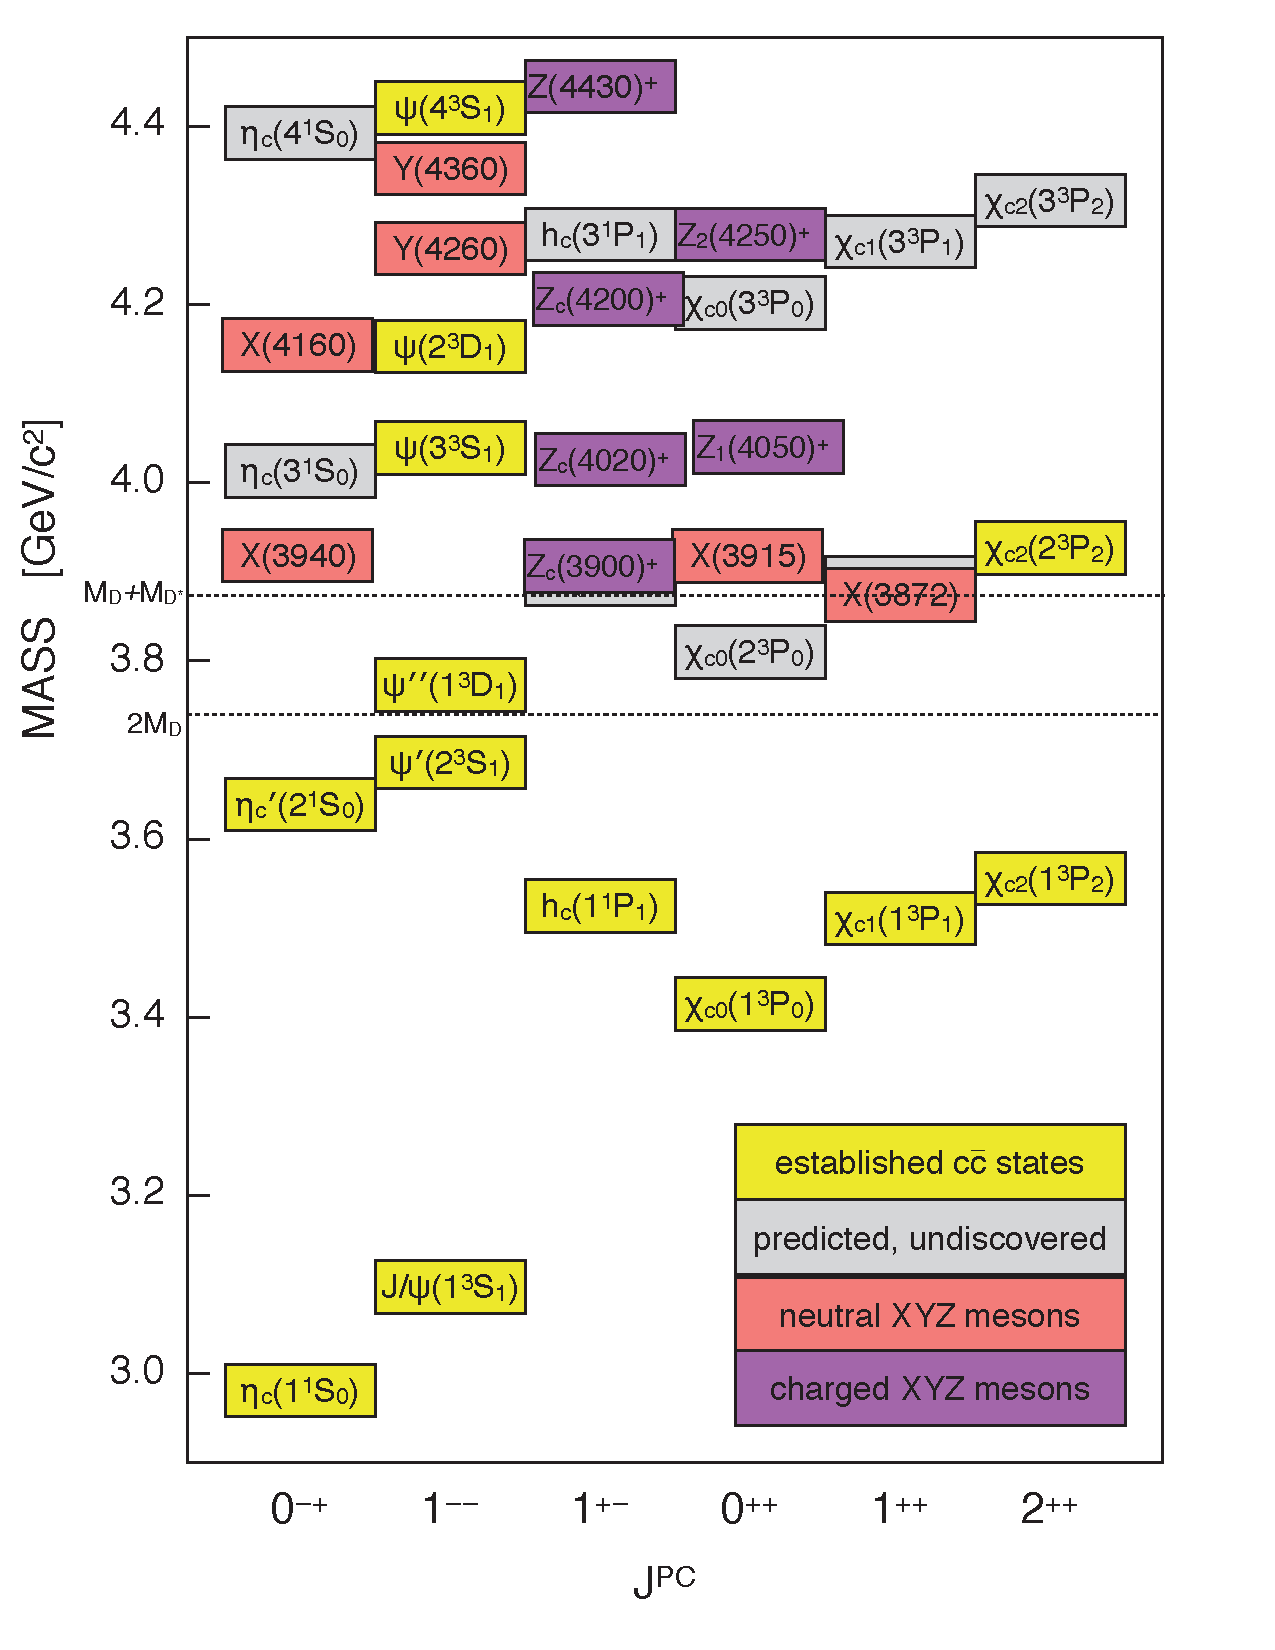
\includegraphics[width=0.85\textwidth]{chap1_charmonium.pdf}
\end{center}
\caption{粲偶素和类粲偶素粒子分布示意图。}
\label{fig:charmonium}
\end{figure}
$\lhcb$实验在运动学区间$y\in$[2.0,4.5]和$\pt\in$[0,14]$\gev$内,对单举$\jpsi$微分产生截面,包括直接产生的和来自$b$强子衰变来的都进行了测量~\cite{Aaij:2011jh}。
对$\psitwos$的测量由于采用了多个重建衰变道,其研究的运动学区间为$y\in$[2.0,4.5]和$\pt\in$[0,14]$\gev$~\cite{Aaij:2012ag}。
同样,对于直接产生的$\psitwos$和来自$b$强子衰变来的$\psitwos$都进行了测量。
如图~\ref{fig:jpsi7TeV}和图~\ref{fig:psitwos7TeV}所示,
在高动量区范围内,NLO NRQCD理论计算与$\lhcb$的测量吻合的很好。
来自$b$强子衰变的$\jpsi$/$\psitwos$的微分截面测量结果与FONLL的预言符合的很好。

\begin{figure}[!tbp]
\centering
\begin{minipage}[t]{0.49\textwidth}
\centering
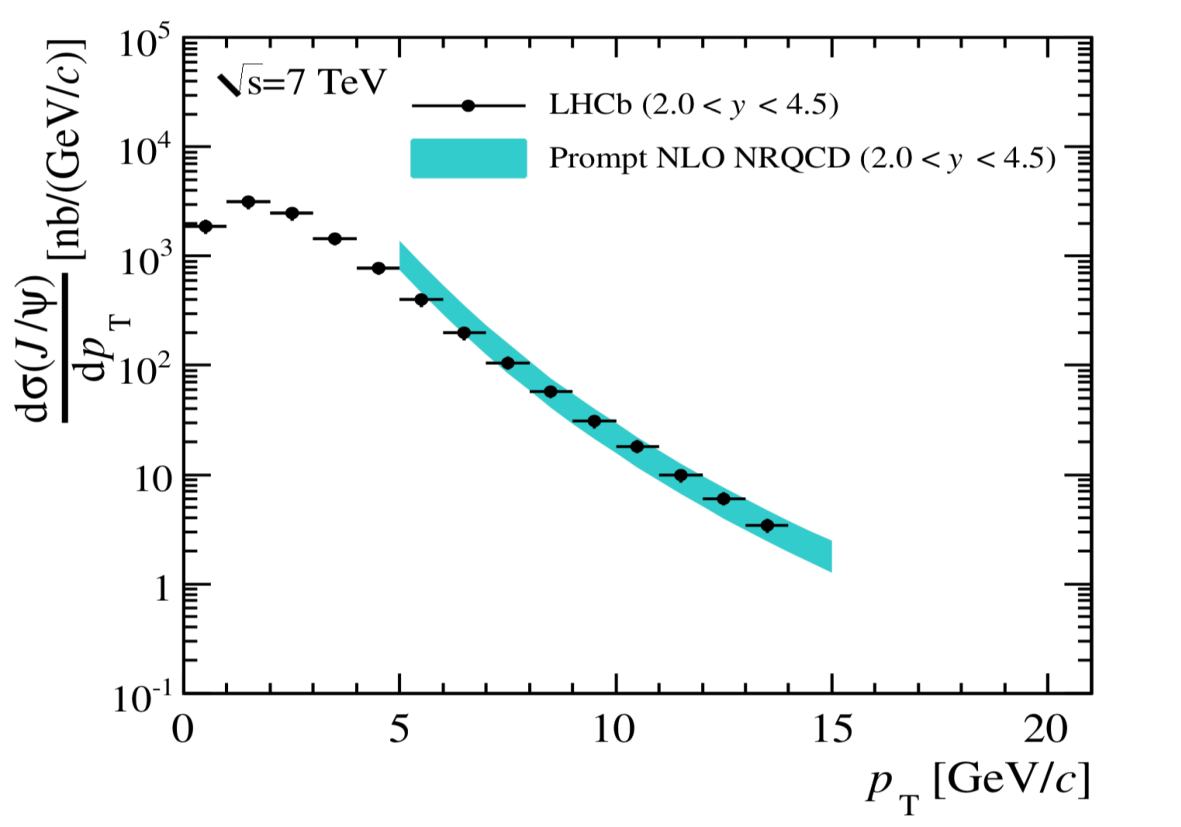
\includegraphics[width=1.0\textwidth]{chap1_jpsi7TeV_prompt}
\end{minipage}
\begin{minipage}[t]{0.49\textwidth}
\centering
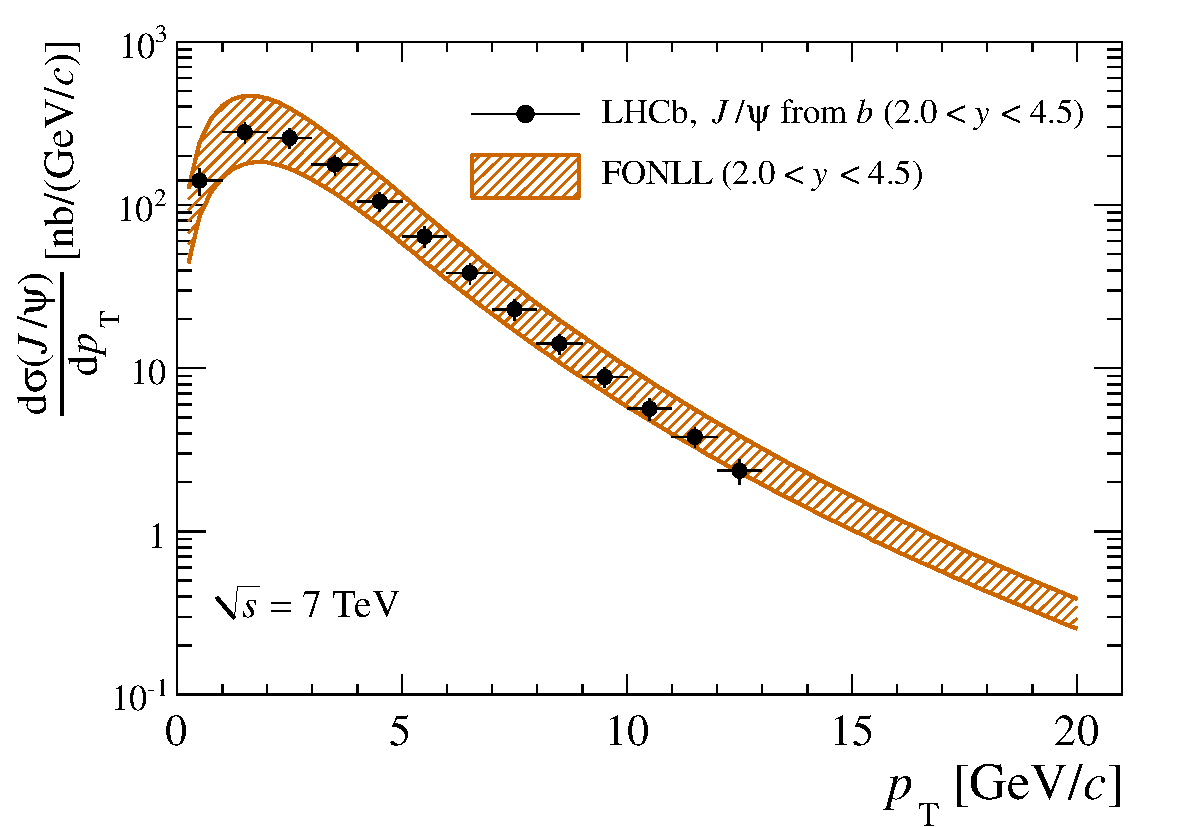
\includegraphics[width=1.0\textwidth]{chap1_jpsi7TeV_bdecay}
\end{minipage}
\caption{质子质子对撞直接产生的$\jpsi$和$b$强子衰变而来的$\jpsi$在7$\tev$下产生截面随着$\pt$的变化。左图为直接产生的$\jpsi$和NRQCD模型计算的对比。右图为$b$强子衰变而来的$\jpsi$与FONLL模型的结果比较。}
\label{fig:jpsi7TeV}
\end{figure}


\begin{figure}[!tbp]
\centering
\begin{minipage}[t]{0.49\textwidth}
\centering
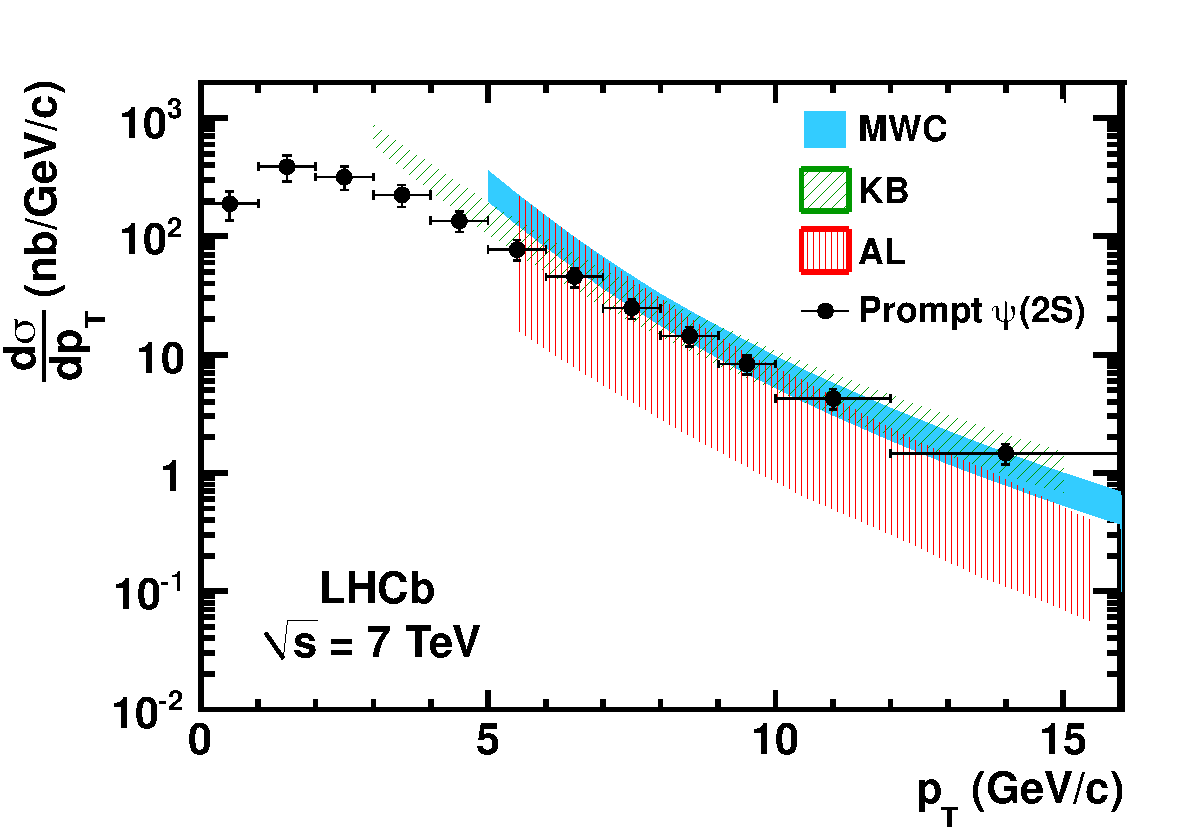
\includegraphics[width=1.0\textwidth]{chap1_psitwos7TeV_prompt}
\end{minipage}
\begin{minipage}[t]{0.49\textwidth}
\centering
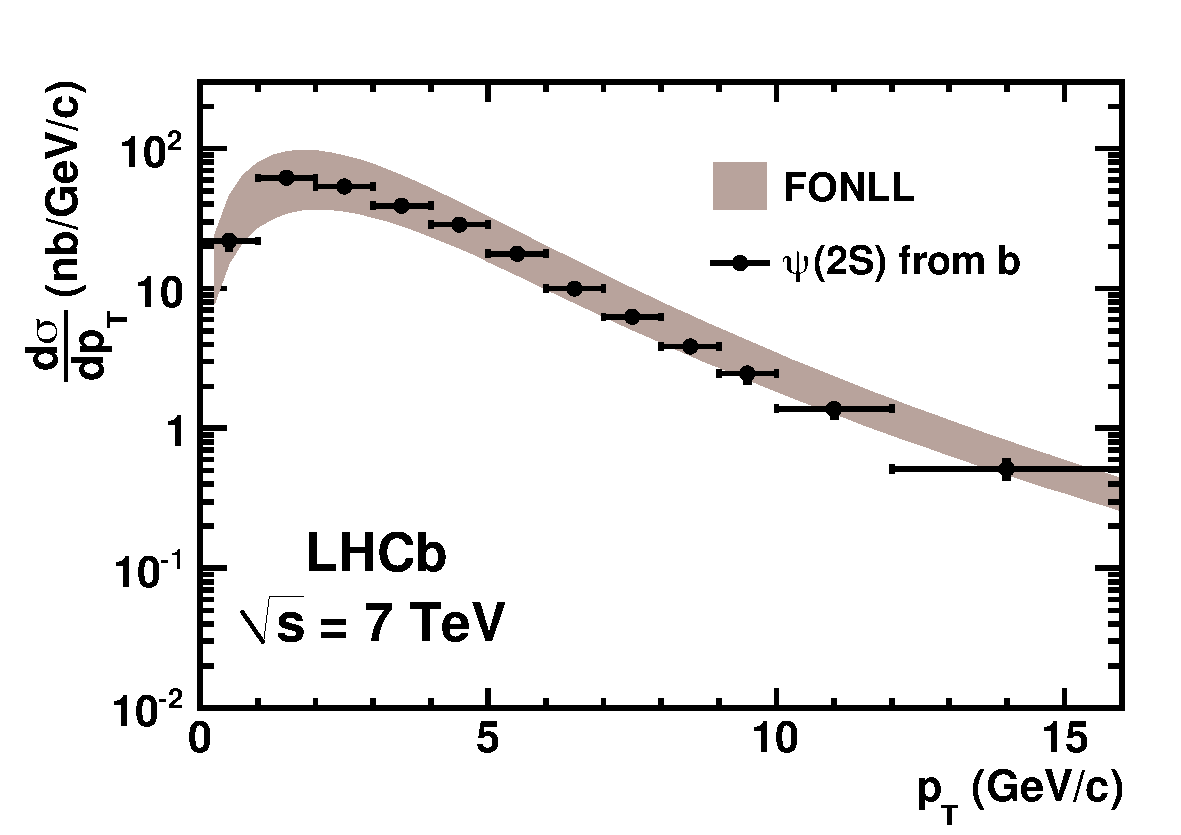
\includegraphics[width=1.0\textwidth]{chap1_psitwos7TeV_bdecay}
\end{minipage}
\caption{质子质子对撞直接产生的$\psitwos$和$b$强子衰变而来的$\psitwos$在7$\tev$下产生截面随着$\pt$的变化。左图为直接产生的$\psitwos$和三种NRQCD模型计算的对比。右图为$b$强子衰变而来的$\psitwos$与FONLL模型的结果比较。}
\label{fig:psitwos7TeV}
\end{figure}

%$\cms$测量了$\Upsilon(nS)$~\cite{Chatrchyan:2012woa}的极化,在误差范围内重夸克偶素没有大的纵向和横向极化。
%$\alice$对$\jpsi$ ~\cite{Abelev:2011md}的极化测量同样表明,在误差范围内夸克偶素没有大的纵向和横向极化。
%
2011年,$\lhcb$ 探测器采集了大约1.0 fb$^{-1}$的质心能量为7 $\tev$ 质子质子对撞的数据。
利用其中约370 pb$^{-1}$的数据,分别在螺旋度参考系和Collins——Soper 参考系,在不同的横动量和快度区间,测量了直接产生的$\jpsi$ 粒子的三个极化参数$\lambda_{\theta}$、$\lambda_{\theta\phi}$ 以及$\lambda_{\phi}$。
在运动学区间2$<\pt<15\gev$,2.0$<y<$4.5,在螺旋度参考系中$\lambda_{\theta}$最小边界$\simeq$ $-$0.2,具有轻微的纵向极化并且随着$\jpsi$ 横动量和快度的增加稍微减少,而$\lambda_{\theta\phi}$和$\lambda_{\phi}$ 在误差范围内近似为0。
利用全部1.0 fb$^{-1}$的数据,$\lhcb$还在螺旋度参考系和Collins——Soper 参考系中测量了直接产生的$\psitwos$的极化参数。
测量结果表明,在误差范围内,在大部分运动学区间$\psitwos$的三个极化参数都近似0,而在某些区域$\psitwos$有轻微的纵向极化,$\lambda_{\theta}$处于$-$0.2到0之间。
如图~\ref{fig:polarization}所示,直接产生的$\jpsi$和$\psitwos$在7$\tev$下极化参数$\lambda_{\theta}$随着$\pt$的变化,并和CSM模型以及三种NRQCD模型计算进行了对比。
结果表明,在$\lhcb$上$\jpsi$和$\psitwos$并不具有很大的横向极化或者纵向极化。
在$\lhcb$和$\alice$探测器共同覆盖的运动学区间内,$\jpsi$的测量结果和$\alice$结果在误差范围内是一致的。
$\lhcb$关于$\jpsi$和$\psitwos$的极化测量不支持领头阶CSM或者NRQCD的理论预言。
目前为止,无论哪种模型都不能同时很好的描述重夸克偶素的微分产生截面和极化~\cite{Knuenz:2015hga},重夸克偶素至今仍然是研究的热点和难点。


基于$\lhcb$在$\sqrt{s}=13\tev$ 处采集的275\,pb$^{-1}$~的$\pp$对撞数据,我们可以在高能量下测量$\psitwos$介子的微分产生截面。
这是在$\lhcb$上7$\tev$质心能量下测量后进行的又一次$\psitwos$微分产生截面的测量。测量采用的大统计量的真实数据保证了测量的更高精度,
测量结果可以很好的检验现有理论模型计算的可靠程度。
结果中对微分产生截面与7$\tev$下$\psitwos$发表结果的比值进行了研究,由于7 $\tev$下$\psitwos$只是发表了随$\pt$ 的变化,所以比值结果只是给出了随$\pt$的变化。
与13$\tev$ 下$\jpsi$结果的比较,可以研究比值随横动量$\pt$、和快度$y$的变化情况。

\begin{figure}[!tbp]
\centering
\begin{minipage}[t]{0.49\textwidth}
\centering
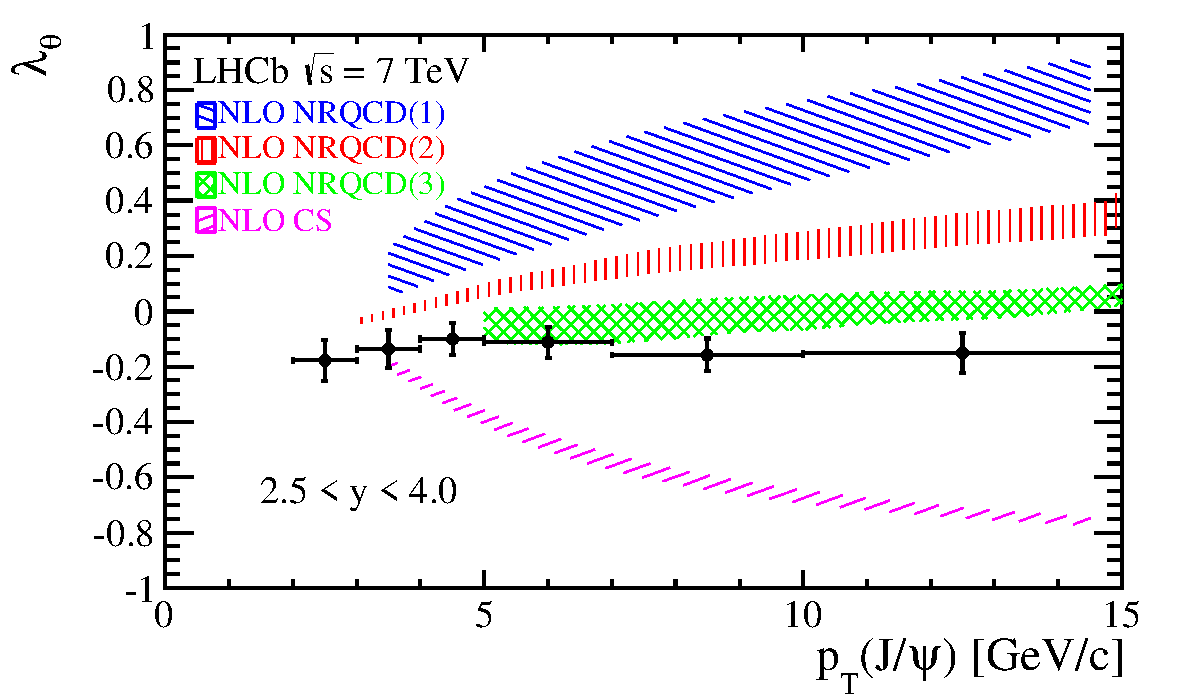
\includegraphics[width=1.0\textwidth]{chap1_polarization_jpsi}
\end{minipage}
\begin{minipage}[t]{0.49\textwidth}
\centering
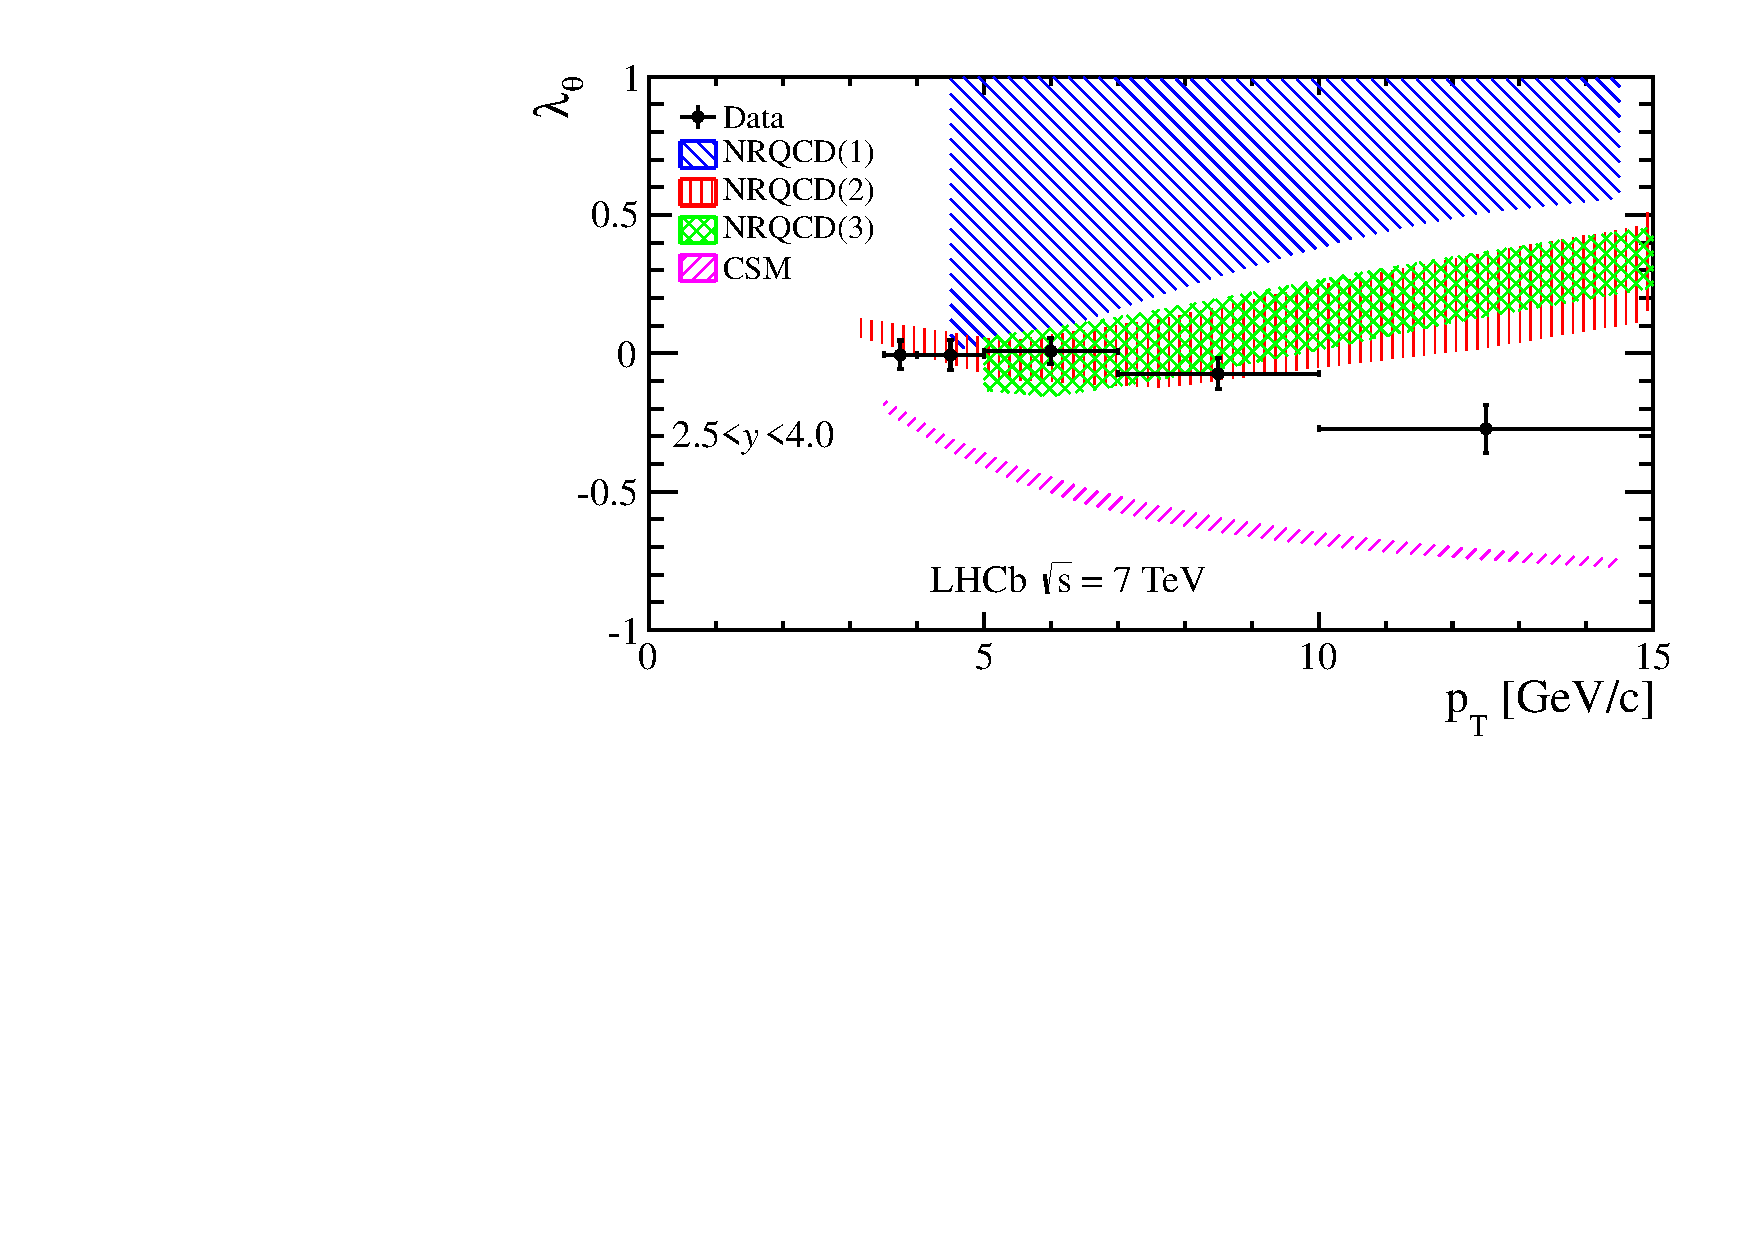
\includegraphics[width=1.0\textwidth]{chap1_polarization_psitwos}
\end{minipage}
\caption{7$\tev$下极化参数$\lambda_{\theta}$随着$\pt$的变化。左图为直接产生的$\jpsi$和CSM模型以及三种NRQCD模型计算的对比。右图为直接产生的$\psitwos$和CSM模型以及三种NRQCD模型计算的对比。}
\label{fig:polarization}
\end{figure}


\section{论文结构}
	本论文结构如下:第一章介绍本论文相关的理论和实验现状,交待选题背景。
	第二章介绍北京正负电子对撞机~BEPCII 和北京谱仪~BESIII。
	第三章介绍BESIII上粲重子$\Lambda^+_c\to \Xi^{(*)0}K^+$的绝对衰变分支比测量。
	第四章详细介绍$\lhcb$上13$\tev$下$\psitwos$介子微分产生截面的测量。
	第五章为总结和展望。

\chapter{北京正负电子对撞机~BEPCII 和北京谱仪~BESIII}
\label{chap:bes3}
北京正负电子对撞机(BEPC)及相应的探测器北京谱仪(BES),在 ~1984 年建成。
1994 年到 1996 年加速器和探测器进行了升级,升级后的对撞机仍称为~BEPC,
而谱仪称为~BESII。
升级后,对撞机和探测器的性能均有了相当大的改进,采集了大量的~$\jpsi$、$\psip$、$\psipp$ 数据,并且对~2.0 $\sim$ 5.0\,GeV 能区进行了扫描,基于这些数据取得了许多重要的物理结果。
例如精确测量$\tau$轻子质量,对$2-5$GeV 的R值精确扫描,系统地研究粲夸克偶素的衰变等等。
从~2004 年开始,通过四年的时间~BEPC 和~BESII 进行了第二次升级改造,
2008年工程竣工,2009年开始物理取数,已经获取了世界上最大的$\tau$-粲能区$\ee$对撞数据样本。
升级后的对撞机和谱仪分别称为~BEPCII 和~BESIII\cite{BEPCBESIII_upgrade}。
现将BESIII上已经获取的实验数据信息列在表~\ref{tab:data}中,几乎所有的样本都是迄今为止世界上同一能量点统计量最大的样本。
本论文的所有研究内容都是基于BESIII探测器上获取到的对撞事例,主要是$XYZ$的数据。

本章主要介绍高能物理实验的特点以及北京正负电子对撞机和北京谱仪上的软硬件结构。

\begin{table}
\centering
\footnotesize
\caption{北京谱仪BESIII上实验数据简介。}
\begin{tabular}{lccc}
\toprule
样本名称 & 质心系能量(GeV) & 亮度或事例数 & 主要物理目标  \\
	\midrule
$\jpsi$数据    & $3.097$ & $13$亿  & 研究$\jpsi$衰变过程中产生的轻强子态性质  \\
$\psip$数据    & $3.686$ & $5$亿  & 研究粲夸克偶素之间的跃迁机制  \\
$\psipp$数据    & $3.773$ & $2.93\rm{fb}^{-1}$  & 研究粲介子的衰变性质  \\
$\tau$轻子质量扫描数据    & $3.554$ & $0.024\rm{fb}^{-1}$  &  $\tau$轻子质量的精确测量  \\
$XYZ$数据    & $3.81-4.599$ & $5\rm{fb}^{-1}$  &  奇特强子态的寻找\\
$R$值和QCD数据    & $2-3$,$3.85-4.59$ & $0.5\rm{fb}^{-1}$,$0.8\rm{fb}^{-1}$  & $R$值精确测量 \\
\bottomrule
\end{tabular}
\label{tab:data}
\end{table}


\section{粒子物理实验介绍}
粒子物理实验又称高能物理实验,主要涉及:粒子源,探测器和数据处理等方面。
早期的粒子源主要是靠来自宇宙的高能粒子射线,人们基本是“靠天吃饭”。
随着加速器技术和电子学技术的发展,人们发展了新的获取粒子源的方法, 也就是利用加速器和对撞机。
现代的粒子物理实验主要就是利用加速器将粒子加速到很高能量,然后使其对撞或打靶发生相互作用,然后用探测器探测末态的次级粒子。
对撞能量越高,能够分辨的空间距离越小,随着人们对微观结构的了解越来越深入,高能物理实验中用到的加速器能量也越来越高。
对撞实验相比于打靶实验的优势在于,两束相对运动的粒子束团对撞提高了有效作用能量,在现在的高能物理实验中,对撞实验占主导地位。

粒子探测器是记录和测量高能粒子信息的工具。高能粒子产生的事例包含不同种类的次级粒子,一般通过探测末态相对稳定的粒子 ($e,\mu,\pi,K,p,n,\gamma$) 来重建中间过程的粒子,还原整个事例的信息。
探测器根据不同粒子和物质相互作用的区别,如图~\ref{fig:tanceqi},探测末态粒子,并区分其种类。
它的具体功能是要测量反应产物的信息(位置、能量、 粒子种类等)。
这些功能通常由多个子探测器来共同完成,比如用漂移室测量带电粒子的轨迹,用电磁量能器测量中性粒子的位置和能量,
用飞行时间计数器测量粒子的飞行时间以判断粒子类型等。
通常把这种需要多个探测器协同工作的大型粒子探测装置称为谱仪。
\begin{figure}
\begin{center}
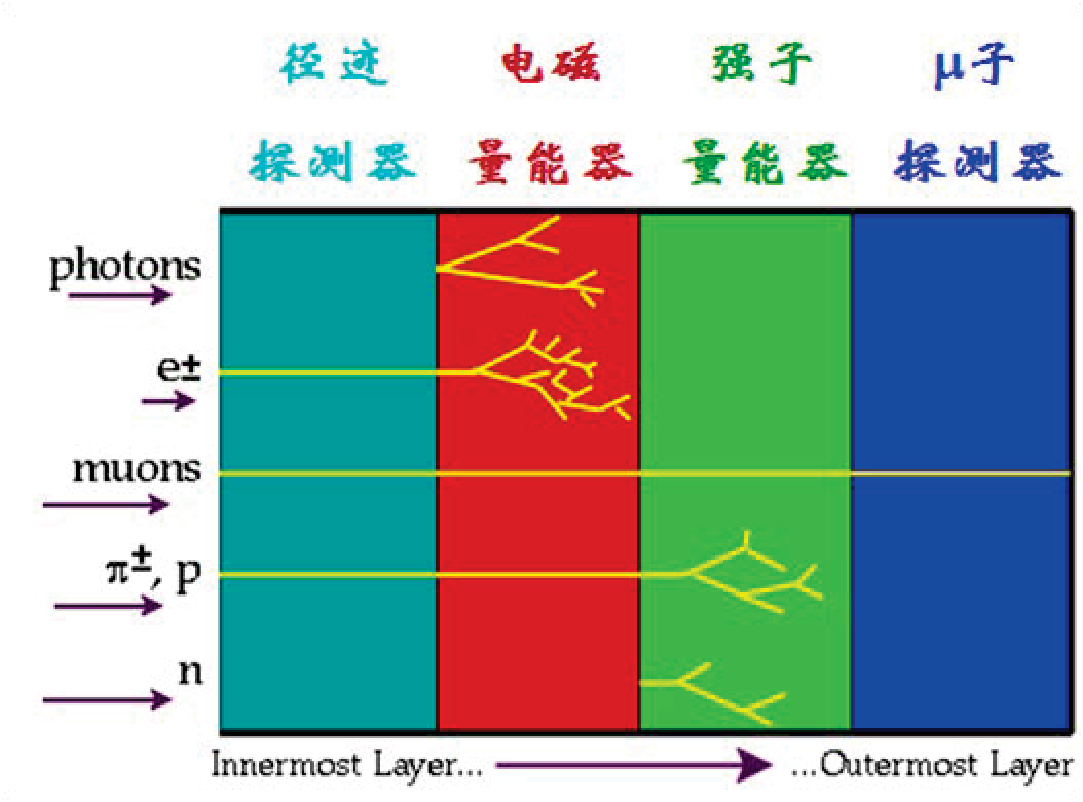
\includegraphics[width=0.5\textwidth]{chap2_general_dector}
\caption{粒子物理实验中探测器的基本工作原理示意。}
\label{fig:tanceqi}
\end{center}
\end{figure}

我们搞粒子物理实验的最终目的是要获得感兴趣的物理结果。通过合理的筛选条件处理实验获取的数据获取感兴趣的事例,就是高能实验物理分析人员要研究的事情。
经常利用粒子的四动量,对不变质量、丢失质量、动量、横动量、空间角分布、时间分布、Dalitz图等进行分析,甚至有时候还需要进行分波分析。
这些分析过程往往都需要蒙特卡洛模拟(Monte Carlo, MC)~\cite{MC}这个重要工具的帮助,以研究信号事例合理的选择条件、分析本底、得到筛选效率等。

当前粒子物理实验的三个研究前沿方向主要是:加速器物理实验的高能量、高亮度和非加速器物理的研究。
\begin{itemize}
  \item 在更高能量下寻找新粒子,探索新的物理模型~\footnote{以欧洲核子中心LHC上的几个实验为主。}。
  \item 在高亮度条件下积累大量数据,用高分辨率探测器进行精确测量,检验标准模型,寻找突破~\footnote{BESIII正是属于这一类。}。
  \item 依靠来自宇宙的高能粒子源,使用巨大体积的探测器,在低背景环境下测量低事例率的物理现象~\footnote{核电站上产生大量中微子,一些人造的非加速器对撞环境提供的粒子源均属此类。}。
\end{itemize}

\section{北京正负电子对撞机}
升级后的北京正负电子对撞机(BEPCII)是工作在$\tau$-粲能区的多束团、高亮度的正负电子对撞机,其峰值亮度比它的前身BEPC高了约两个量级。
BEPC主要由注入器,束流输运线和储存环组成。注入器是一台长202\ m的直线加速器,由电子枪产生的电子,和电子打靶产生的正电子,
被直线加速器加速后由束流输运线注入到储存环。储存环是一台环形加速器,束流在环内积累、加速、储存和对撞~\cite{BEPCII}。
BEPCII利用原有的储存环隧道,采用双环方案,使正负电子束流在两个彼此独立的储存环中积累和加速,在对撞点处对撞。
双环结构是保证亮度提高两个量级的关键选择。
BEPCII的主要性能参数列于表~\ref{tab:BEPCII}。
值得一提的是该论文完成前不久的2016年4月5日,BEPCII的亮度达到了其设计亮度$1 \times 10^{33}\rm{cm}^{-2}s^{-1}$,为工作在该能区的加速器亮度之最。
此外,北京正负电子对撞机还做到了所谓的“一机两用”,可以运行的同步辐射模式下,作为同步辐射的光源。
\begin{table}
\centering
%\footnotesize
\caption{BEPCII的主要设计参数。}
\begin{tabular}{ll}
\toprule
束流能量$E_{b}$(GeV)               &  $1.0\sim2.3$  \\
设计亮度($E_{b}$=1.89\ GeV)        &  $1 \times 10^{33}\rm{cm}^{-2}s^{-1}$ \\
高频频率(MHz)                      & 499.8 \\
对撞周期(ns)                       & 8 \\
储存环长度(m)                      & 237.53 \\
束团数目                             & 93 \\
正负电子注入速率(mA/min)           & 50 \\
\bottomrule
\end{tabular}
\label{tab:BEPCII}
\end{table}

\begin{figure}
 \centering
 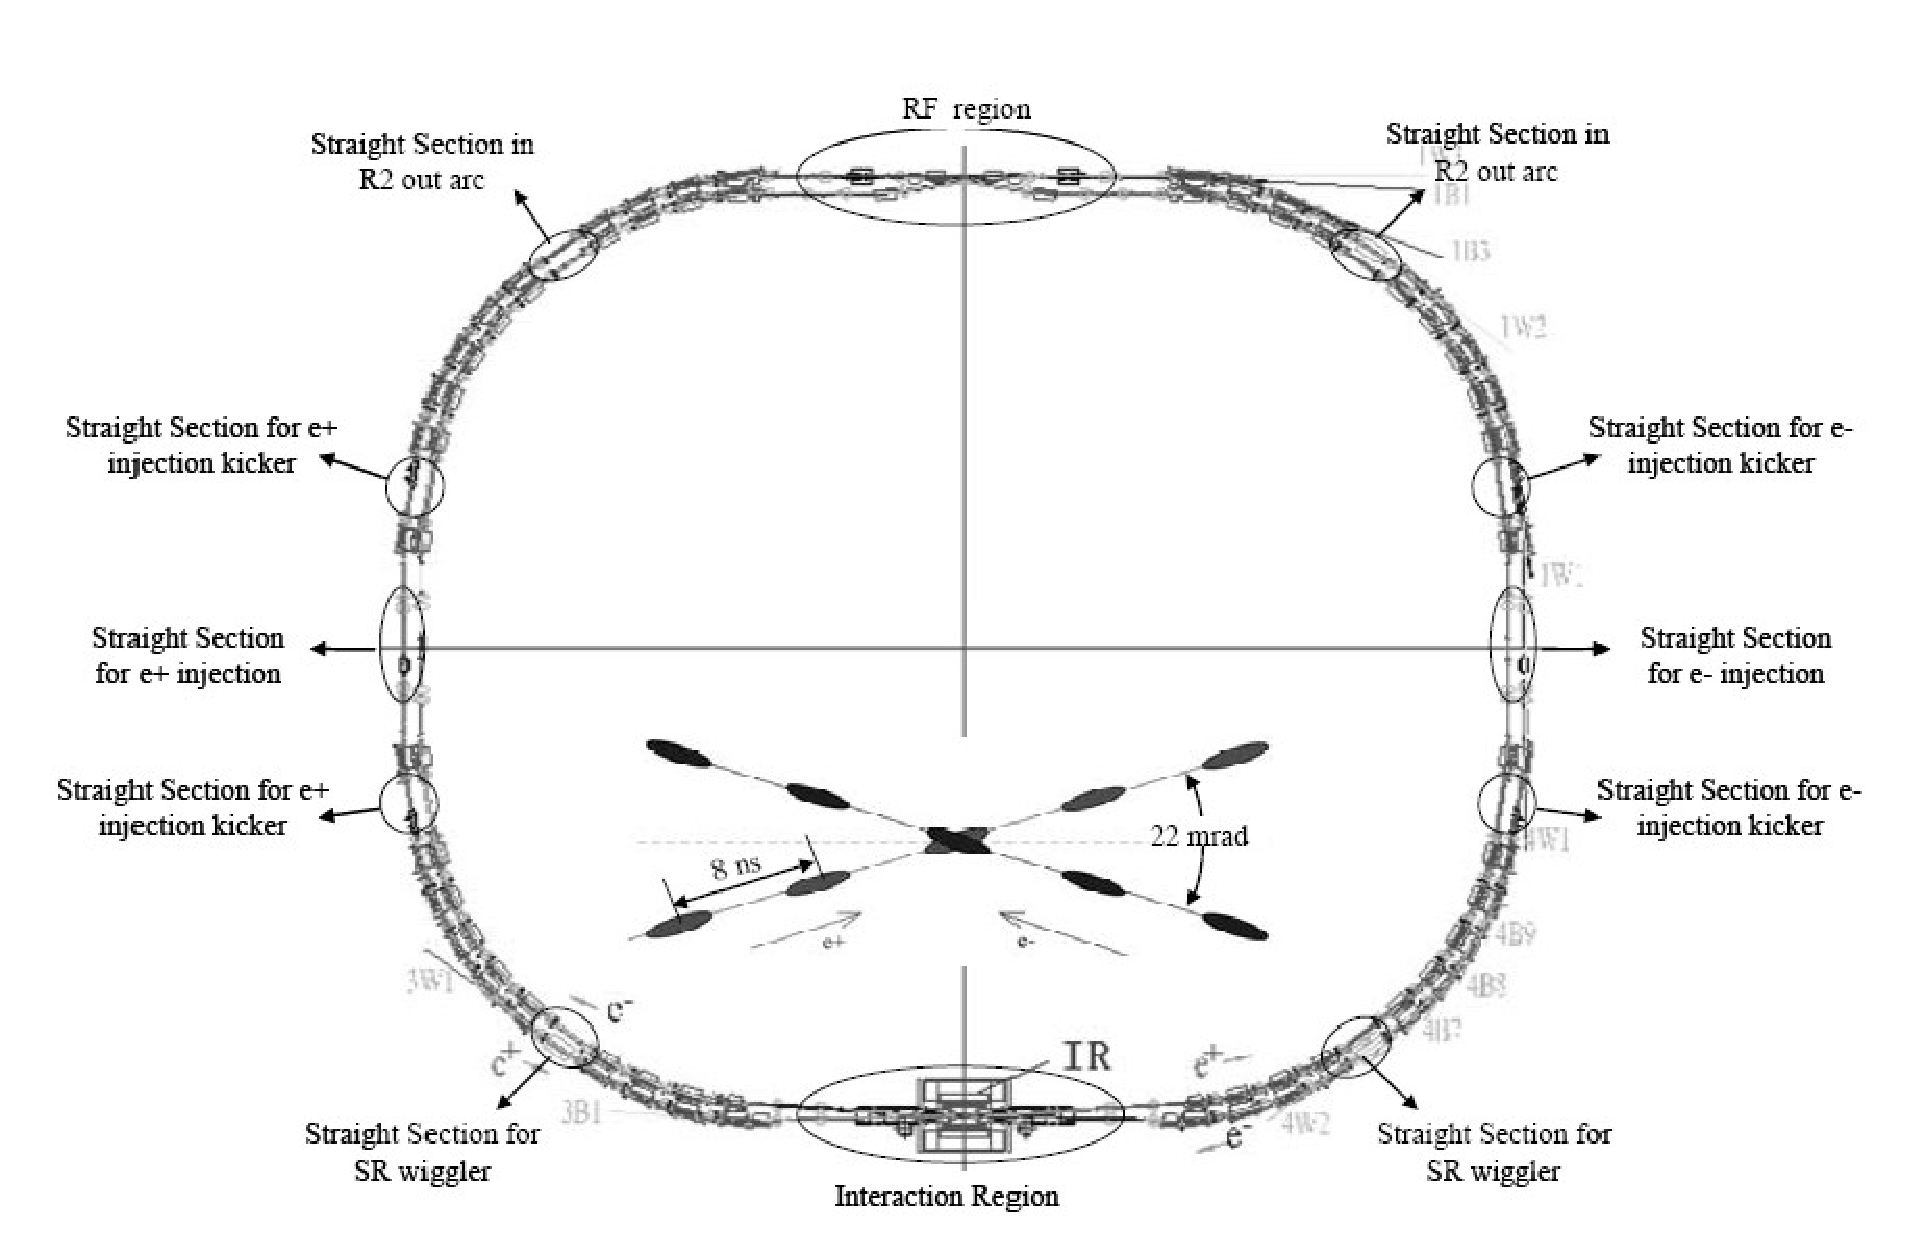
\includegraphics[width=0.8\textwidth]{chap2_BEPCII}
 \caption{BEPCII俯视图。}
 \label{fig:BEPCII}
\end{figure}

\section{北京谱仪}
北京谱仪(BESIII)是运行在BEPCII上采用现代探测技术的大型通用探测器,用于探测$e^{+}e^{-}$对撞产生的末态粒子。
BESIII工作在所谓的$\tau$-粲能区,该能区是精确检验标准模型和寻找新物理的理想场所。
BESIII的物理目标包括$\tau$-粲能区弱电相互作用的研究、强相互作用研究及新物理的寻找等~\cite{Asner:2008nq}。

BESIII将对弱电相互作用理论进行精确检验:利用$D$和$D_{s}$介子衰变精确测量CKM矩阵元,检验其幺正性;
通过精确测量$\tau$轻子质量对轻子普适性进行更高精度的检验;在$\tau^+\tau^-$近域高精度的截面测量更好地理解$\tau^+\tau^-$间的相互作用;
利用$\lambdacp\lambdacm$阈值上的优势,精确测量$\lambdacp$的强衰变和半轻衰变性质。

在强相互作用领域,由于$\tau$-粲能区强相互作用的非微扰特性,使得目前在该能区几乎所有的理论计算都有很大的不确定性。
利用$\tau$-粲能区的数据对QCD的研究主要包括:
结合高精度的LQCD的计算进行标准模型基本参数的测量,如强相互作用耦合常数$\alpha_{s}$等;测量低能强子谱, 寻找QCD预言的各种含胶子的态,如胶子球、混杂态等;
研究粲偶素的产生和衰变性质,检验和发展量子色动力学的各种计算。 

BESIII 持续高亮度的运行,使得其能够积累大量的数据,从而可以进行稀有衰变的测量,如对味道改变中性流 (FCNC)的寻找, 测量结果相对预期值的反常偏离都预示着新的机制或者新物理的贡献;还可以对非标准模型过程进行寻找,如轻子数或重子数破坏的过程。
另外,标准模型中~$D^{0}-\bar{D^{0}}$ 的混合以及~$D_{s}$/$D$ 衰变中的~CP 破坏效应都很小,而新物理的贡献可以加强这种效应。
在~BESIII 上测量中性~$D$ 介子的混合及~$CP$ 破坏,都可以用来寻找新物理或对新物理的贡献给出一个限制。


为了达到上面提到的物理目标,BESIII 探测器必须满足以下要求:
\begin{itemize}
\item 能够探测低动量的带电粒子,并精确测量其动量和方向;
\item 好的粒子鉴别能力,能够区分开各种粒子,如电子、$\mu$~子、质子、$\pi$~介子、$K$~介子等;
\item 精确测量光子,具有非常好的能量分辨、角度分辨及光子识别能力;
\item 前端电子学系统、触发系统以及数据获取系统要适应~BEPCII 多束团模式下的高事例率取数,尽量减少死时间。
\end{itemize}

基于以上要求,BESIII 探测器的总体结构如图~\ref{fig:BESIII}所示。
由内向外依次为主漂移室(Main Drift Chamber, MDC)、飞行时间计数器(Time of Flight, TOF)、CsI电磁量能器(Electro-Magnetic Calorimeter, EMC)、 超导磁体(Superconductor Magnet)和$\mu$子计数器(Muon Counter, MUC)。
表~\ref{tab:bes3p}给出了BESIII探测器的主要性能参数~\cite{BESIII}。

\begin{figure}
 \centering
 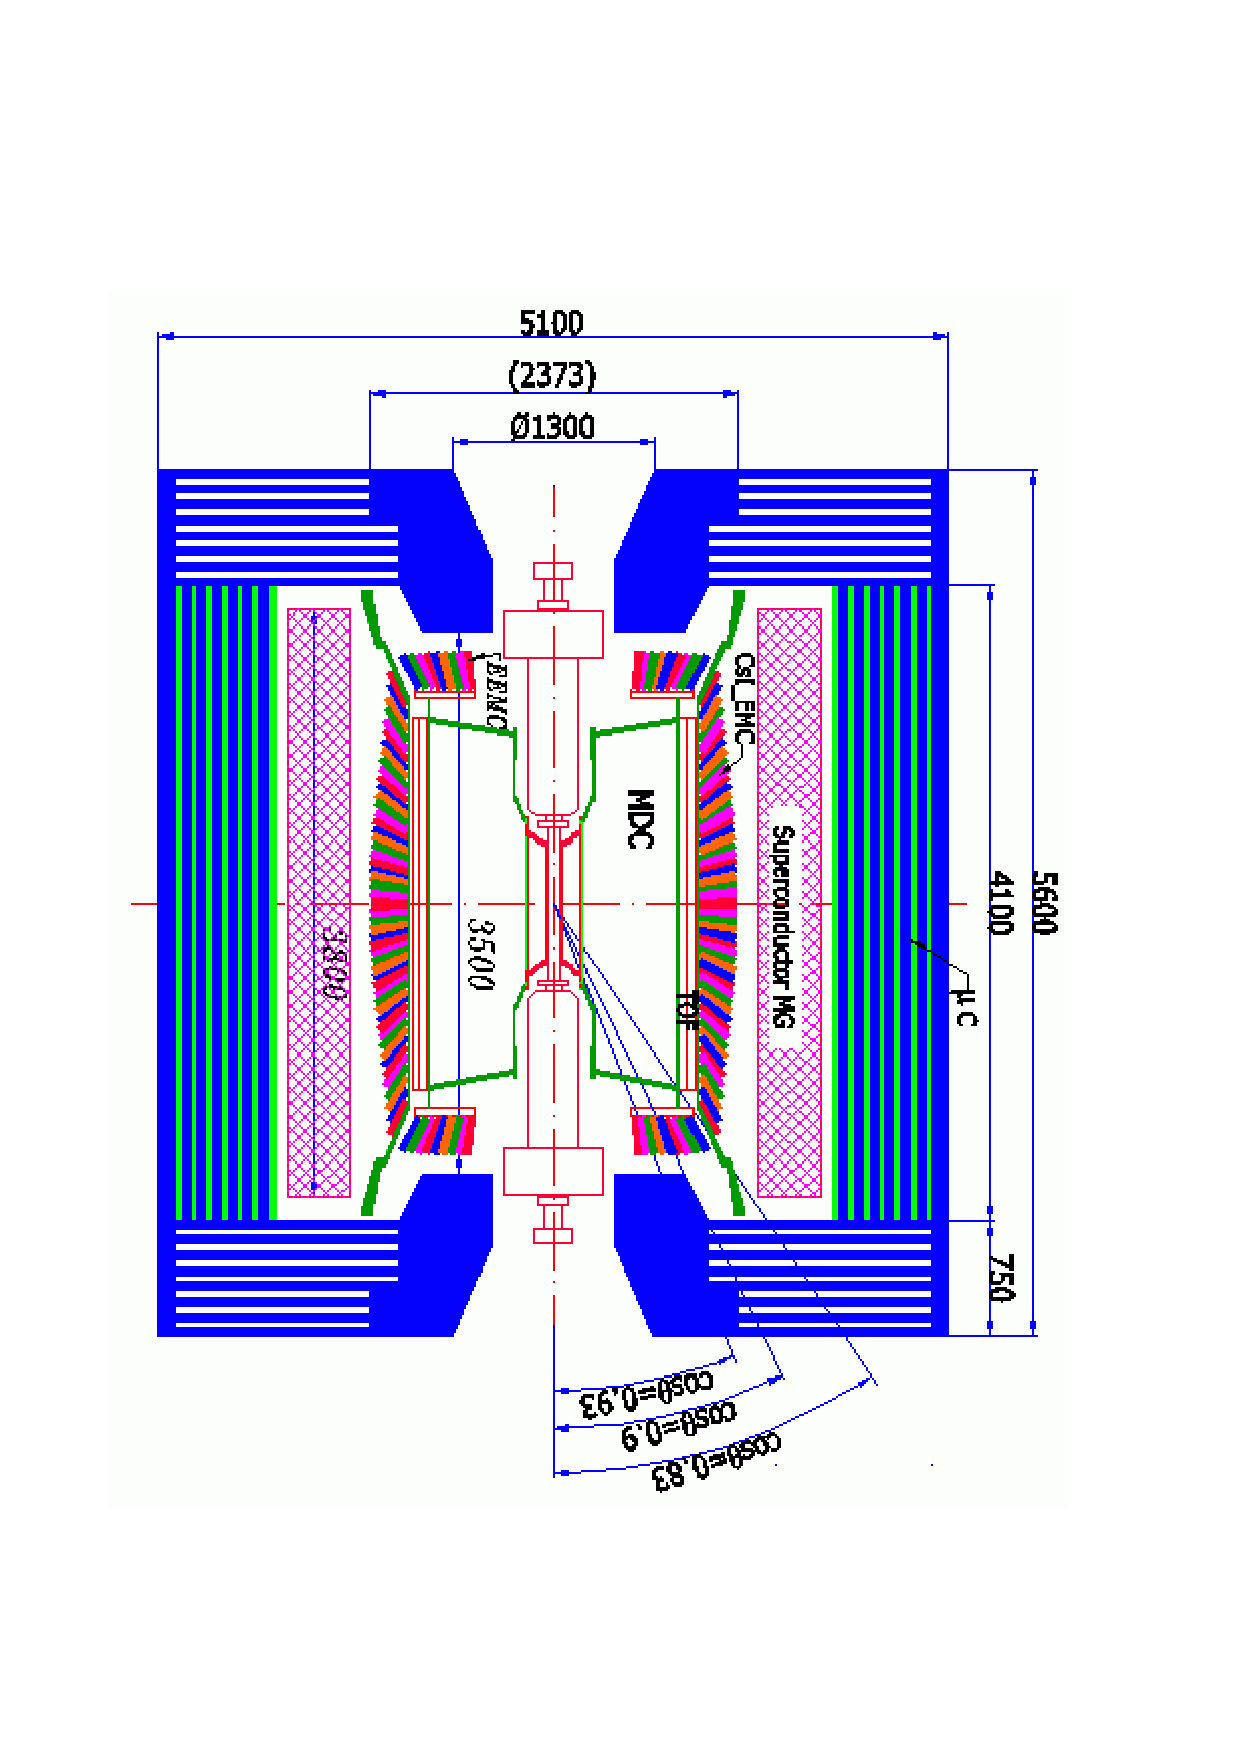
\includegraphics[angle=90,width=0.8\textwidth]{chap2_bes_view}
 \caption{BESIII探测器的结构侧视图。}
 \label{fig:BESIII}
\end{figure}


\begin{table}
\centering
\footnotesize
\caption{BESIII主要性能参数。}
\begin{tabular}{ll}
\toprule
子系统                         & 主要性能参数 \\
\midrule
\multirow{3}* {主漂移室}       & $\sigma_{xy}$=130\ $\mu$m            \\
                               & $\Delta P$/{\it{P}}=0.5\ \% @1.0\ GeV     \\
                               & $\sigma_{dE/dx}$=6-7\ \%              \\
\midrule
\multirow{2}* {飞行时间计数器} &  $\sigma_{t}$= 90\ ps 桶部  \\
                               &  $\sigma_{t}$= 110\ ps 端盖  \\
\midrule
\multirow{2}* {电磁量能器}     &  $\Delta E$/{\it{E}}=2.5\ \% @1.0\ GeV  \\
                               &  $\sigma_{\phi z}$=0.6\ cm  @1.0\ GeV  \\
\midrule
$\mu$ 子计数器                 &   9\ 层   \\
磁场强度                       &   0.9 $\sim$ 1.0\ T \\
\bottomrule
\end{tabular}
\label{tab:bes3p}
\end{table}

\section{小结}
本章简要介绍了BEPCII和BESIII的结构、BESIII 各个子系统的结构性能和指标等。

\chapter{BESIII实验上粲重子$\LtoXiXisK$的绝对分支比测量}
\label{chap:lambdac}

关于粲重子$\lambdacp$测量的背景情况我们在前言部分已经详细阐述过了,这里不再赘述。
重点提一下我们数据采集的能量点。
如图~\ref{fig:lambc_cs_belle}和图~\ref{fig:lambc_cs_bes3}所示,在各质心系能量下$\lambdacp\lambdacm$对过程产生的截面,在4.6$\gev$的质心系能量下Belle实验测量的结果为$\sigma(\ee\to\lambdacp\lambdacm)=0.38\pm0.13\,\rm{nb}$~\cite{Pakhlova:2008vn},BESIII初步的测量结果为$\sigma(\ee\to\lambdacp\lambdacm)=0.237\pm0.015\,\rm{nb}$~\cite{Ablikim:2017lct}。

\begin{figure*}[h]
\centering
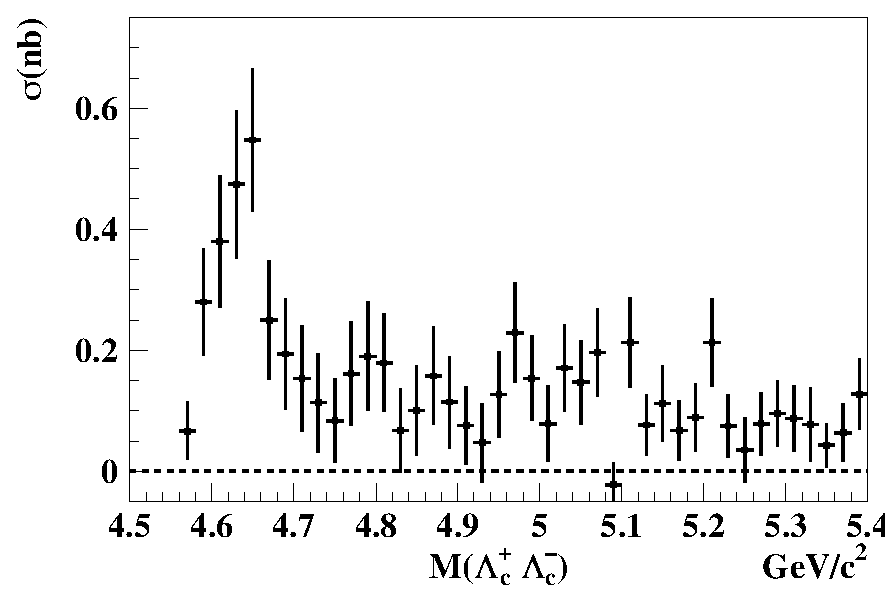
\includegraphics[width=0.85\textwidth]{chap2_LcLc_lineshape_belle}
\caption{ BELLE 实验测量的$\ee\to\lambdacp\lambdacm$ 的截面。}
\label{fig:lambc_cs_belle}
\end{figure*}

\begin{figure*}[h]
\centering
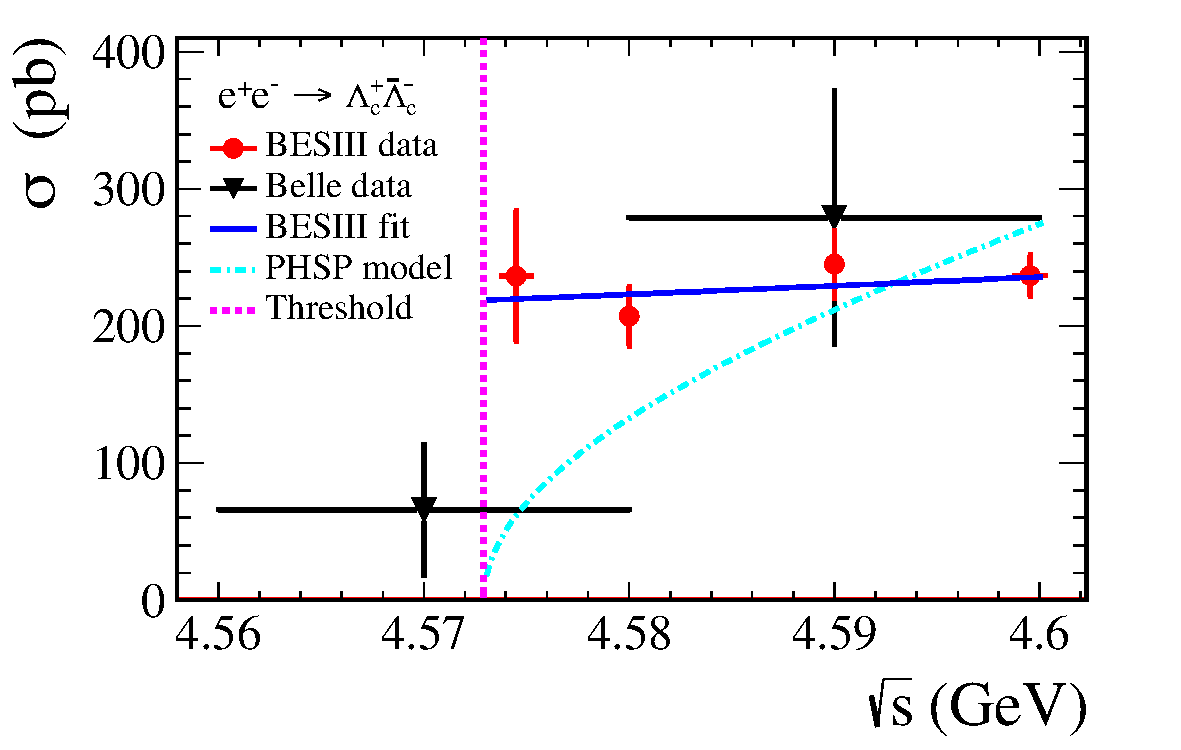
\includegraphics[width=0.85\textwidth]{chap2_LcLc_lineshape}
\caption{ BESIII 实验初步测量的$\ee\to\lambdacp\lambdacm$ 的截面。}
\label{fig:lambc_cs_bes3}
\end{figure*}
2014年BESIII在4.6$\gev$的质心系能量下进行取数,共积累了567$\rm{pb}^{-1}$的$\lambdacp\lambdacm$阈值数据。
我们知道$\lambdacp\lambdacm$的质量阈值为4573$\mev$,该能量点略高于$\lambdacp\lambdacm$对质量阈值26$\mev$左右。
注意到4.6$\gev$依然不是$\lambdacp\lambdacm$截面的峰值,但这却已经远远超过了北京正负电子对撞机II设计的最高能量4.2$\gev$。
不得不说BESIII实验能在$\lambdacp\lambdacm$的质量阈值以上采集数据这是BEPCII的巨大成功。
因为阈值上的数据本底简单,运动学约束的也比较好,同样情况下大家更愿意去相信阈值上数据给出的结果。
这批数据为我们研究测量$\lambdacp$的性质提供了一个非常好的平台。


\section{测量方法}
\label{sec:method}
我们一共挑选了11个分支比较大的所谓的~Cabibbo~允许的强子衰变道
$\Lmodea$, $\Lmodeb$, $\Lmodec$, $\Lmoded$, $\Lmodee$, $\Lmodeaa$, $\Lmodebb$, $\Lmodedd$, $\Lmodeaaa$, $\Lmodeccc$, $\Lmodeddd$~和~1个重建效率比较高的~Cabibbo~压制的$\Lmodee$~\footnote{除非特别说明,否则本文中所指的衰变道均暗含着电荷共轭道在内的。}。
其中$\Ks,\pizero,\Lambda,\Sigma^0$和$\Sigma^+$这些不是稳定可探测粒子,对于这些中间共振态我们选择如表~\ref{tab:interDecay} 所示的重建方式且引用其在PDG中的分支比结果。

\begin{table}
%\footnotesize
\caption{中间共振态的重建方式及其分支比。}
\centering
\begin{tabular}{c|c}
\hline \hline
衰变方式 &分支比(\%) \\ \hline
$\Ks \to \pip\pim$  &    $69.20\pm 0.05$   \\ 
$\pizero \to \gamma\gamma$       &   $98.823\pm 0.034$    \\
$\Lambda \to p\pim$       &   $63.9\pm 0.5$    \\
$\Sigma^0 \to \Lambda\gamma$       &   $100$    \\
$\Sigma^+ \to p\pizero$       &   $51.57\pm 0.30$    \\
%$\omega    \to \pip\pim\pizero$        &    $89.2\pm 0.7$  \\
\hline
\end{tabular}
\label{tab:interDecay}
\end{table}

我们选择使用双标记的方法来对分支比$\mathcal{B}(\LtoXiXisK)$进行测量。这种方法是由MARK III合作组首次提出来的~\cite{mark3a,mark3b}。
简述一下双标记方法的原理:
如图~\ref{fig:topopkpi}所示$\lambdacp\lambdacm$成对产生。
\begin{figure*}[h]
\centering
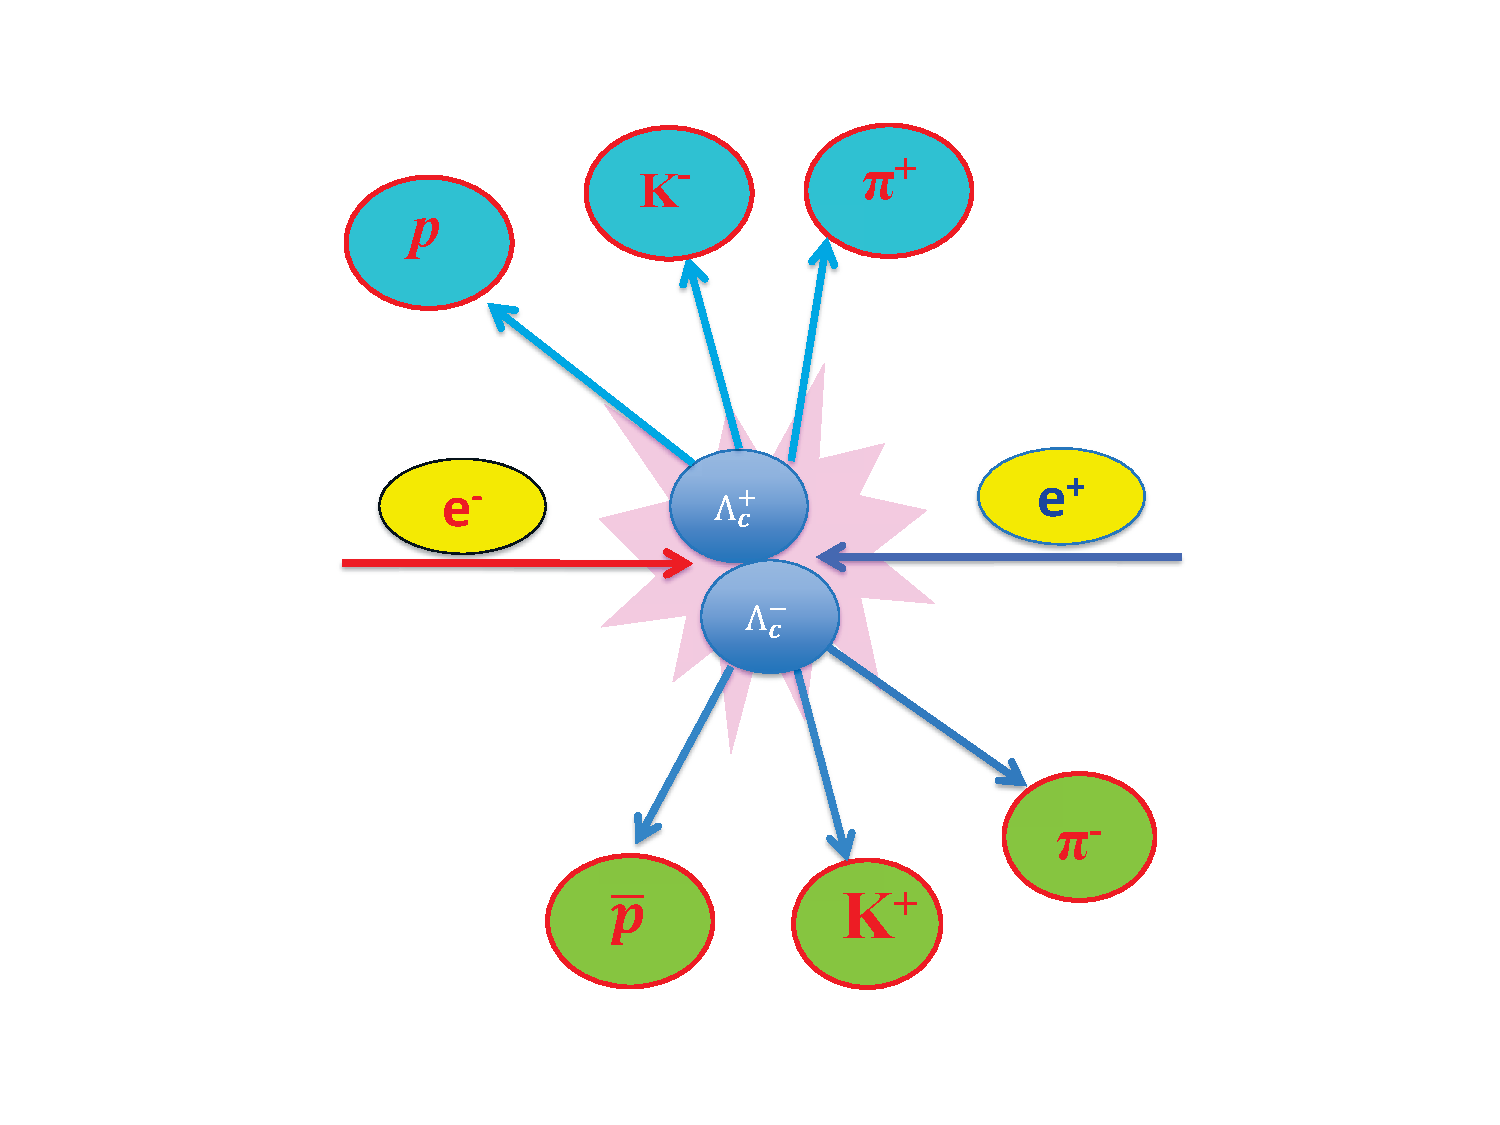
\includegraphics[width=0.4\textwidth]{chap2_topo_pkpi}
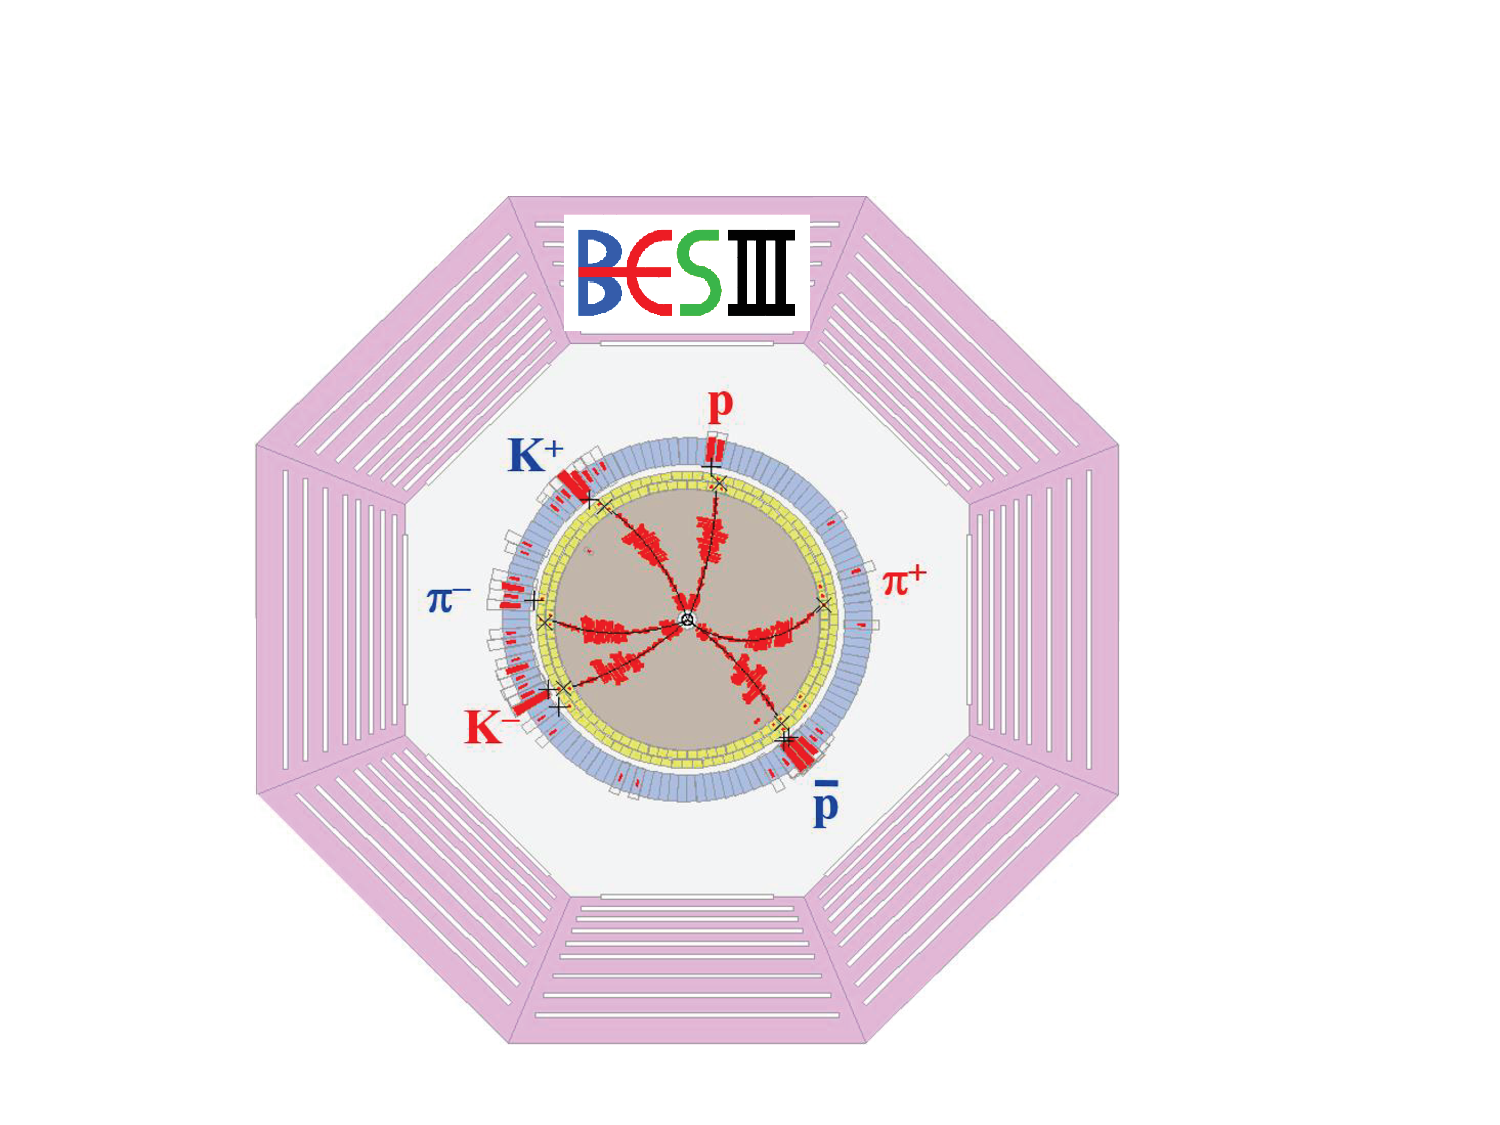
\includegraphics[width=0.4\textwidth]{chap2_evtdisplay_pkpi}
\caption{ BESIII 实验上成对产生的$\lambdacp\lambdacm$。 }
\label{fig:topopkpi}
\end{figure*}
我们首先在所有的末态径迹中只重建一个$\lambdacm$,称之为{\it 单标记事例}。
然后我们在单标记$\lambdacm$的反冲侧的末态里面再去重建$\XiXisK$,这称之为{\it 双标记事例}。
则$\LtoXiXisK$的绝对衰变分支比可以通过单标记事例的产额、双标记事例的产额、单标记事例的效率和双标记事例的效率四者之间比例关系求出,
而不需要知道$\lambdacp\lambdacm$事例产生的总数。
举个具体的例子,比如我们想用衰变道$i$作为标记道去测量衰变道$\LtoXiXisK$的分支比。
首先,用$N_{i}^{ST}$来表示$\lambdacp$衰变到这个衰变道$i$的产额,则
\begin{eqnarray}
N_{i}^{\rm ST}&=&N_{\lambdacp\lambdacm}\cdot\mathcal{B}_{i}\cdot\varepsilon_{i}^{\rm ST},
\label{eq:st}
\end{eqnarray}
其中,$N_{\lambdacp\lambdacm}$指的是数据中应有的$\lambdacp\lambdacm$对的总数,
 $\mathcal{B}_{i}$指的是$\lambdacm$衰变到衰变道$i$的分支比,$\varepsilon_{i}^{\rm ST}$指的是这个标记道的重建效率。
对于双标记事例我们指定$\lambdacm \to i$ 并且 $\LtoXiXisK$,故双标记产额$N_{i,\XiXisK}^{\rm DT}$可以表示为:
\begin{eqnarray}
N_{i,\XiXisK}^{\rm DT}&=&N_{\lambdacp\lambdacm}\cdot\mathcal{B}_{i}\cdot\mathcal{B}(\LtoXiXisK)\cdot\varepsilon_{i,\XiXisK}^{\rm DT},
\label{eq:dt}
\end{eqnarray}
其中$\varepsilon_{i,,\XiXisK}^{\rm DT}$指的是$\lambdacm \to i$ 并且 $\LtoXiXisK$同时被重建出的效率,称作双标记效率。
对公式~\ref{eq:st}和公式~\ref{eq:dt}进行简单的代数运算可以得到计算$\LtoXiXisK$的分支比公式:
\begin{eqnarray}
\mathcal{B}(\LtoXiXisK) &=& \frac{N_{i,\XiXisK}^{\rm DT}}{N_{i}^{\rm ST}}\cdot\frac{\varepsilon_{i}^{\rm ST}}{\varepsilon_{i,\XiXisK}^{\rm DT}}.
\label{eq:ratio}
\end{eqnarray}

这种测量分支比的方法称为“ 绝对(absolute)分支比 ” 测量,这种方法的突出优点是:
\begin{itemize}
  \item 不需要知道$\lambdacp\lambdacm$的总数;
  \item $\frac{\varepsilon_{i,\XiXisK}^{\rm DT}}{\varepsilon_{i}^{\rm ST}}$,消掉了很多单标记侧的系统误差,提高了测量的精度。
\end{itemize}

具体到我们这个分析中$\LtoXiXisK$绝对衰变分支比的测量,由于单个双标记产额$N_{i,\XiXisK}^{\rm DT}$的数目太少,所以我们将12个单标记道对应的双标记产额加在一起来处理,将公式\ref{eq:st}和公式\ref{eq:dt}联立并且求和,有如下公式:
\begin{eqnarray}
N_{-,\XiXisK}^{\rm DT}&=&\sum_{i}N_{i,\XiXisK}^{\rm DT}=\mathcal{B}(\LtoXiXisK)\cdot\sum_{i}(\frac{N_{i}^{\rm ST}}{\varepsilon_{i}^{\rm ST}}\cdot\varepsilon_{i,\XiXisK}^{\rm DT}).
\label{eq:br}
\end{eqnarray}
公式\ref{eq:br} 就是我们直接计算分支比的公式。

从上面的讨论中可以看出整个分析流程我们只要知道单标记事例的产额$N_{i}^{\rm ST}$、双标记事例的产额$N_{i,\XiXisK}^{\rm DT}$、单标记事例的效率$\varepsilon_{i}^{\rm ST}$和双标记事例的效率$\varepsilon_{i,\XiXisK}^{\rm DT}$即可对分支比进行计算,接下来的章节就是去阐述怎么去获取上述这些数值。

\section{实验数据和MC模拟样本}
\label{sec:sample}
本分析使用BESIII在BOSS6.6.4p01下重建下的2014年3月份在质心系能量$\sqrt{s}=4.6\gev$处采集的数据,总的积分亮度为567\,pb$^{-1}$~\cite{Ablikim:2015nan}。 

我们使用Monte Carlo (MC)模拟样本来理解本底和估计探测效率。
对于探测器的模拟我们使用非常成熟的GEANT4~\cite{ref:geant4a,ref:geant4b}软件包。
MC模拟的时候我们使用KKMC~\cite{Jadach:2000ir}考虑束流的能散和初态辐射以及带电粒子的末态辐射效应。
为了满足本分析的需要我们模拟产生了如下3类的MC样本:

\begin{itemize}
    \item Cocktail MC 事例: 用来研究本底情况和估计效率。包含BESIII官方产生的MC样本~\cite{pingrg_mc}还有根据我们自己的需求又大量模拟的一些。这里将此类样本总结到表~\ref{tab:MCsample}中,并且列出与数据中该过程的事例数(亮度)比例关系。对于部分QED过程如$\ee$、$\mu^+\mu^-$和$\gamma\gamma$,由于其对我们要研究的衰变过程均无贡献故未列出。需要指出的一点是$\lambdacp\lambdacm$过程是我们最关心的过程,从而进行了大量的模拟且分成了均等的两份:一份用来估计单标记道的重建效率;另一份用来做输入输出检查。
    \item 单标记信号形状MC:顾名思义就是用这份MC样本来获取用来拟合的信号形状。我们要求单标记侧$\lambdacp$ ($\lambdacm$)衰变到12个信号道,另外一侧的$\lambdacm$ ($\lambdacp$)严格地衰变到$e^{-}+\overline{\nu}_{e}$($e^{+}+\nu_{e}$),这样模拟MC的目的是为了得到一份干净的信号MC形状,因为这样另外一侧的末态粒子可以认为是不会对单标记侧造成任何影响的。我们一共模拟了150万个该过程的事例。

    \item 双标记信号MC:用来获取双标记事例的效率。 我们要求两侧的$\Lambda_c$都衰变到12个信号道。由于双标记选择效率较低,为了减小由于模拟统计量有限导致的效率误差我们共产生了大量该过程事例。
\end{itemize}

以上所述各种MC所有涉及$\ee \to \lambdacp\lambdacm$过程的,初态辐射波恩截面是按照BESIII所测结果图~\ref{fig:lambc_cs_bes3}放进EVTGEN考虑了的,并且$\lambdacp$或者$\lambdacm$次级衰变的模型是按照我们在数据中观测到的模式进行模拟的。
\begin{table}
\footnotesize
\caption{Cocktail MC 包含的各个物理过程,相应的截面及其与数据的比例关系。}
\centering
\begin{tabular}{l|c|c|c|c}
\hline \hline
物理  & 截面  & $567\,\rm{pb}^{-1}$的数据 & MC模拟 & MC是数据 \\ 
过程  & (nb)  & 中的事例数($10^6$) & 事例数($10^6$)  & 的倍数 \\ \hline
$\lambdacp\lambdacm$ & 0.178\protect\footnotemark  & 0.1009  & 3.874+3.874  &  38.4+38.4  \\ \hline 
DD & 3.3  & 1.8711  & 4.94  &  2.64  \\ \hline 
qqbar & 16  & 9.072  & 10.9  &  1.2  \\ \hline 
$\tau^+\tau^-$ & 3.4  & 1.9278  & 9  &  4.67  \\ \hline 
ISR 到较轻$\psi$态 & 0.67  & 0.38  & 4  &  10.5  \\ \hline 
\hline
\end{tabular}
\label{tab:MCsample}
\end{table}
\footnotetext{此处截面值为4.6$\gev$处的观测截面,区别于图~\ref{fig:lambc_cs_bes3}中所示波恩截面。}



\section{事例选择条件}
\label{sec:selection}
在物理分析过程中,经常利用探测器记录的末态粒子的相关信息,通过刻度和重建计算出带电径迹和中性径迹的径迹参数,并鉴别带电径迹的粒子类型,然后利用这些末态径迹重建出衰变过程中产生的各种中间共振态($\Ks,\pizero,\Lambda,\Sigma^0$和$\Sigma^+$)。
本节将详细的介绍好的带电粒子和好的中性粒子的鉴别方法,以及各种中间共振态的选择,见图~\ref{fig:intermediate}。
%%%%%%%%%%%%%%%%%%%%%%%%%%%%
\begin{figure*}[hp]
\centering
\subfigure[数据中$\pi^{0}$ 不变质量分布。]
{
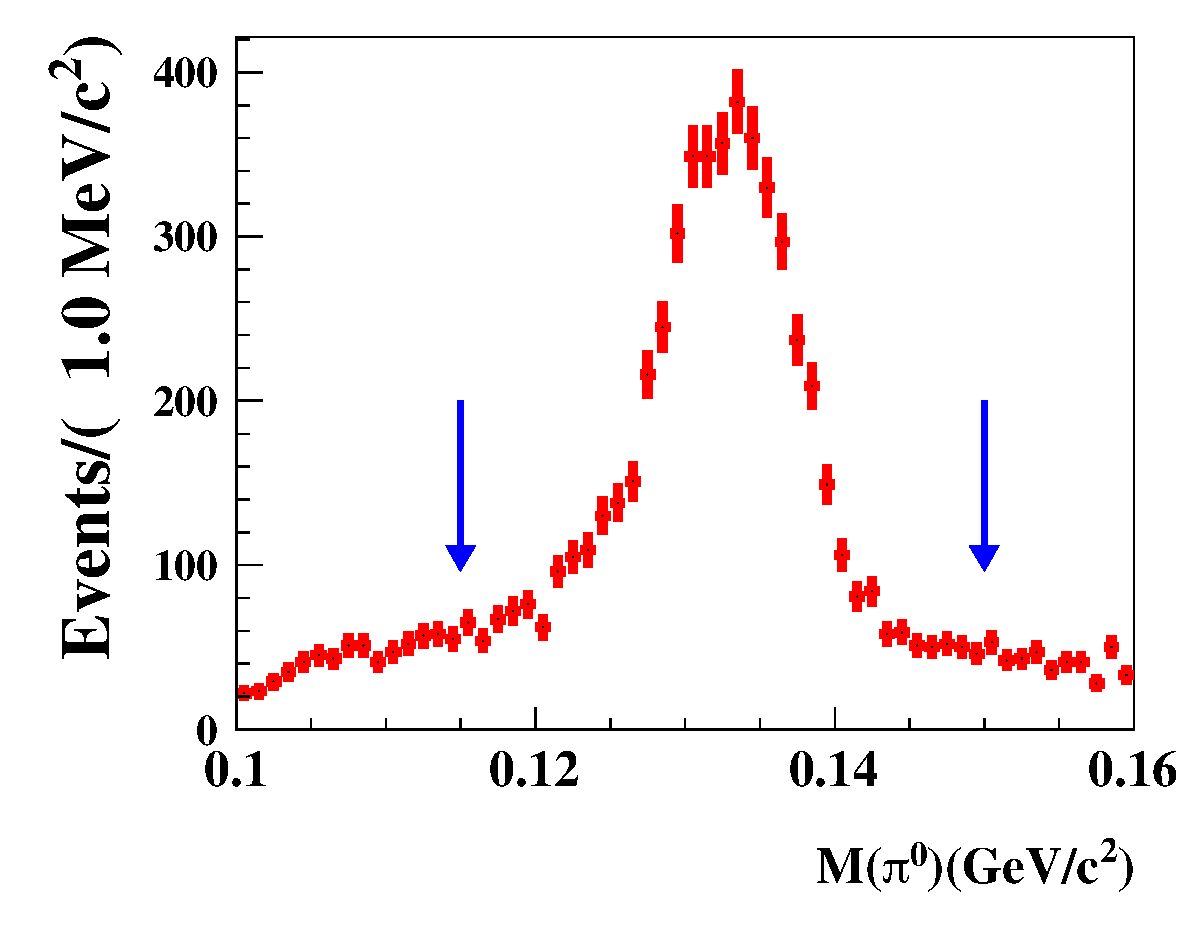
\includegraphics[width=0.45\textwidth]{chap2_m_pi0}
\label{fig:pi0mass}
}
\hspace{10pt}
\subfigure[数据中$K_{S}^{0}$ 不变质量分布。]
{
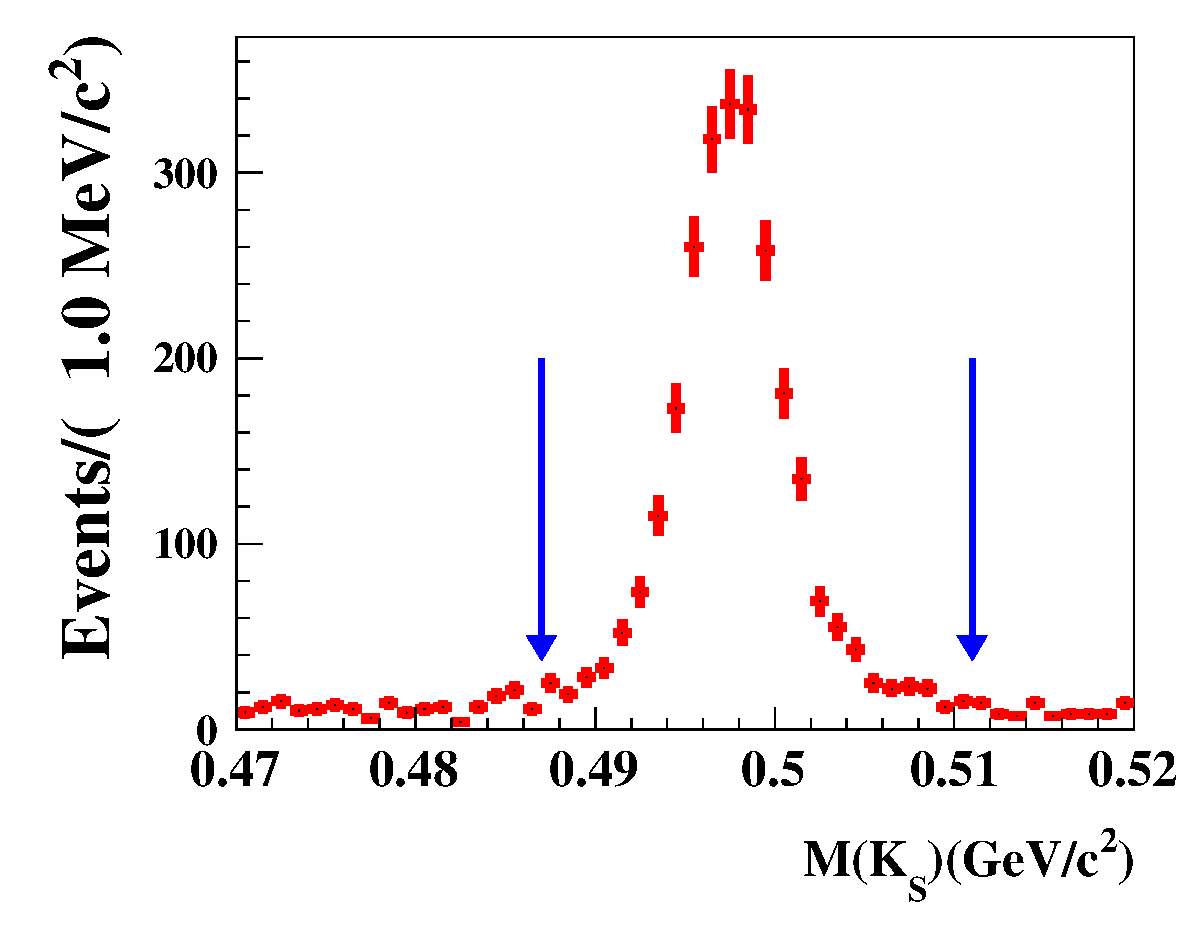
\includegraphics[width=0.45\textwidth]{chap2_m_Ks}
\label{fig:Ksmass}
}
\subfigure[数据中$\Lambda$ 不变质量分布。]
{
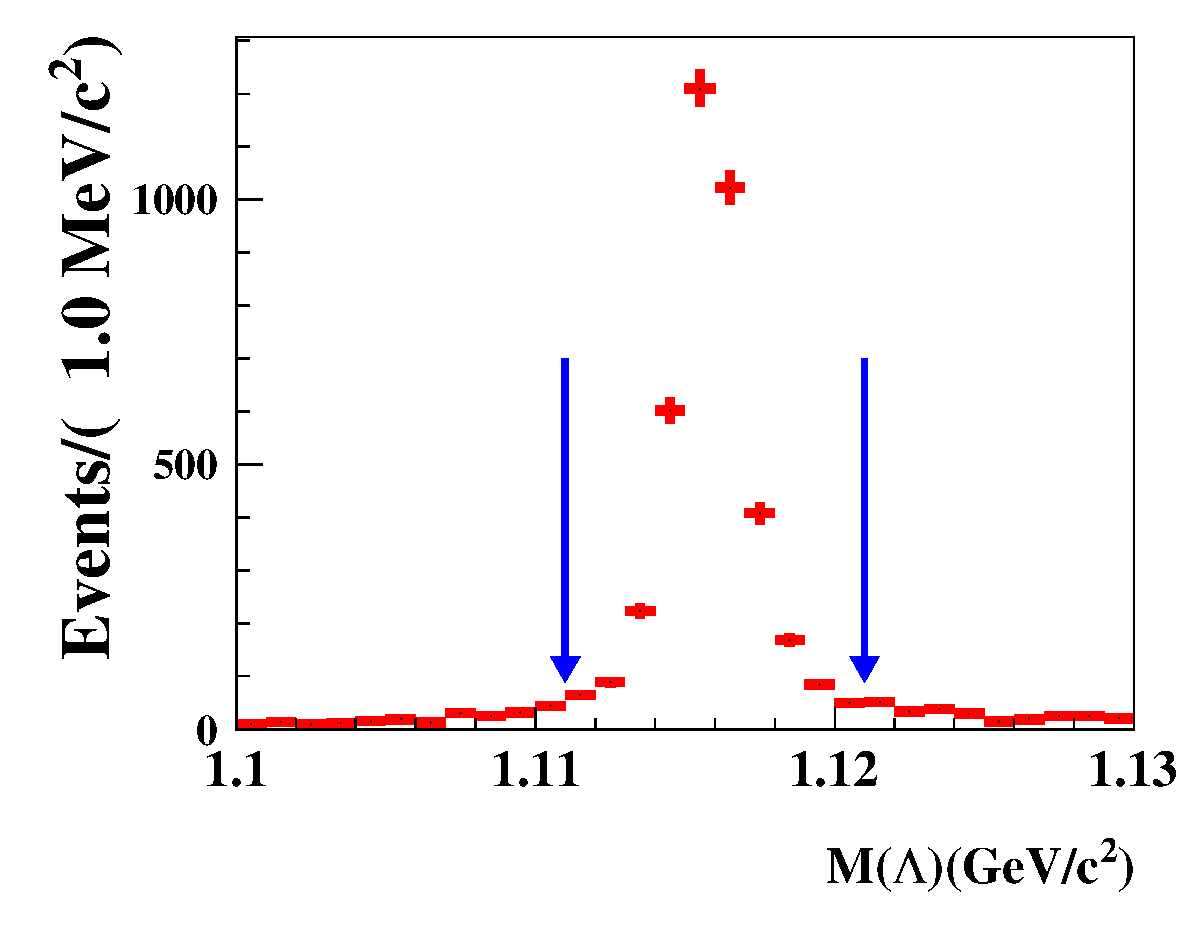
\includegraphics[width=0.45\textwidth]{chap2_m_lmd}
\label{fig:lmdmass}
}
\subfigure[数据中$\Sigmazero$ 不变质量分布。]
{
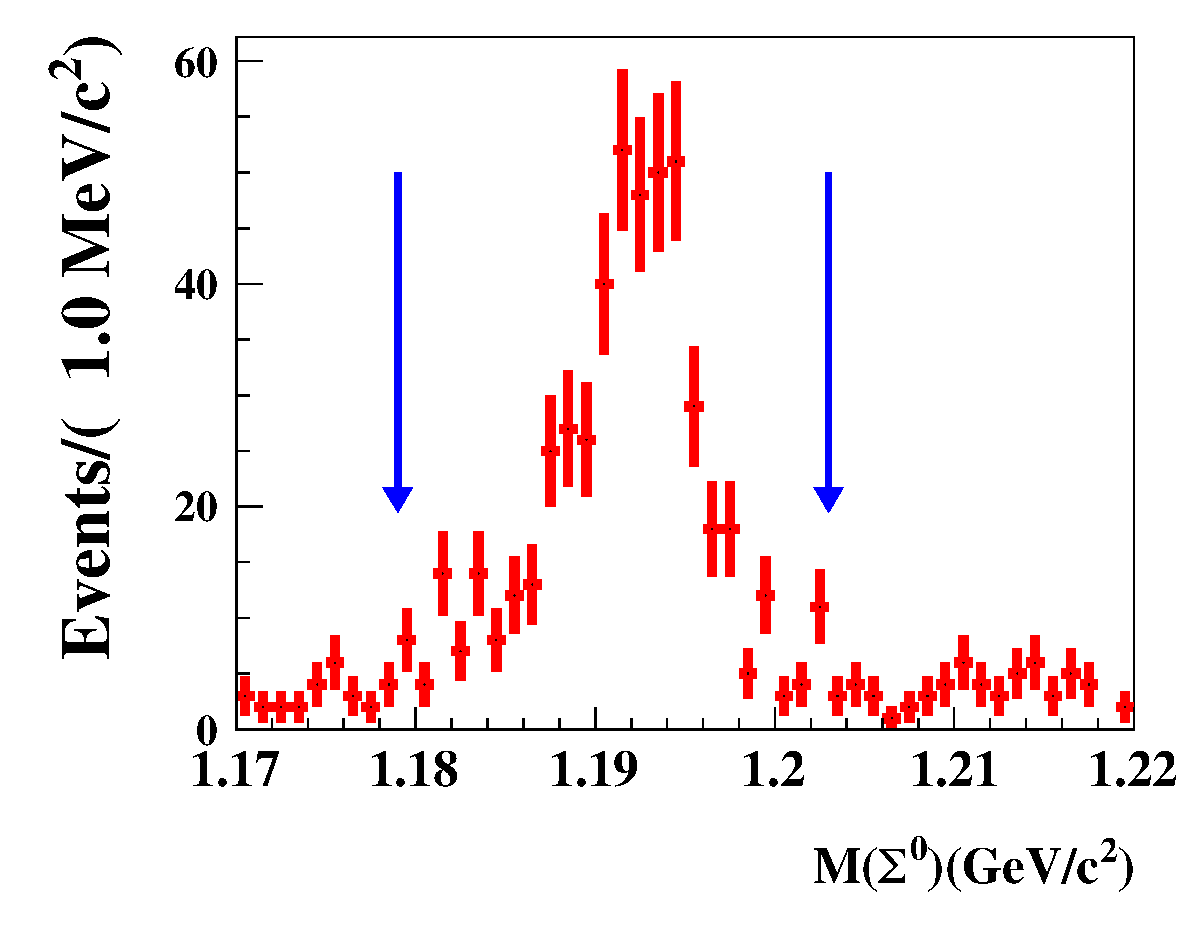
\includegraphics[width=0.45\textwidth]{chap2_m_Sgm0}
\label{fig:Sgm0mass}
}
\subfigure[数据中$\Sigmap$ 不变质量分布。]
{
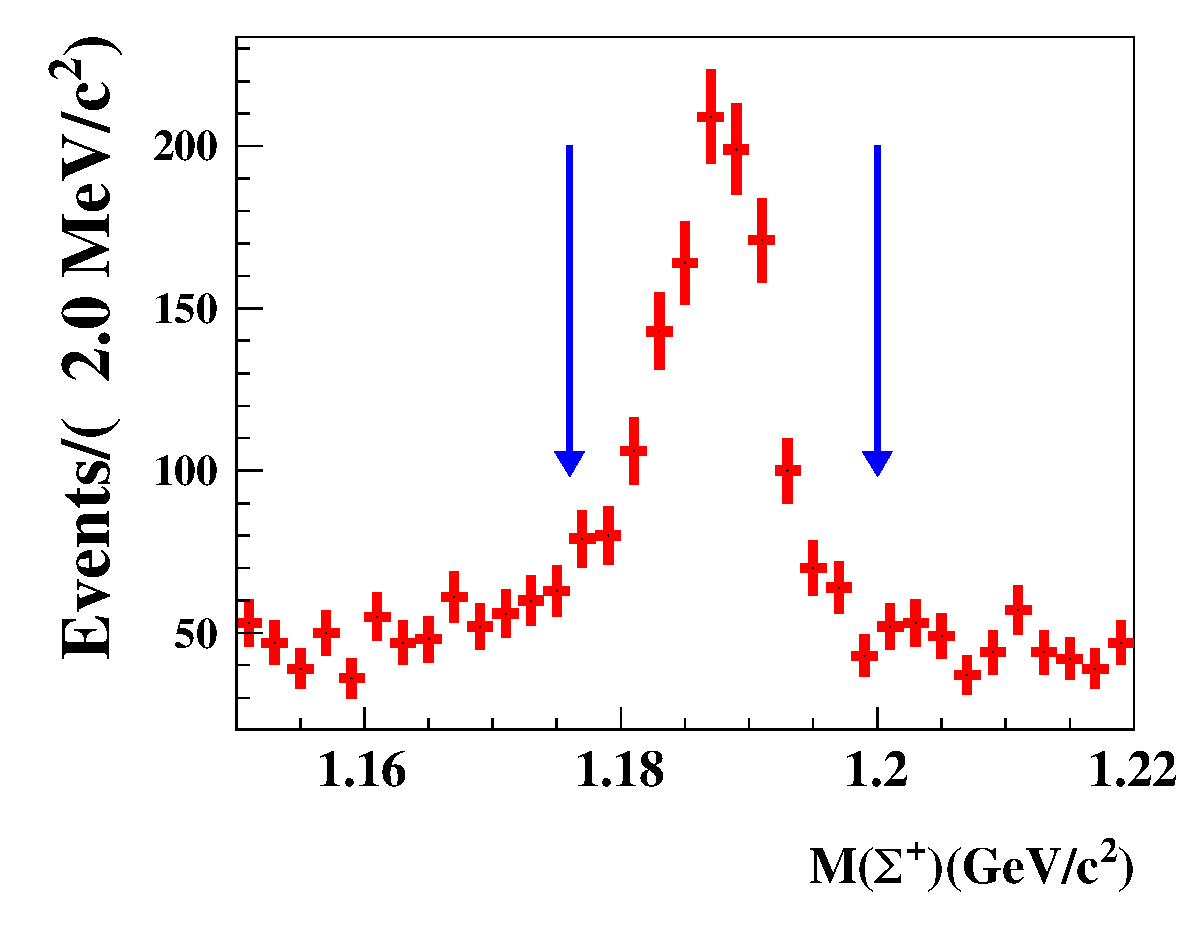
\includegraphics[width=0.45\textwidth]{chap2_m_Sgmp}
\label{fig:Sgmpmass}
}
\caption{数据中各中间共振态的不变质量谱的分布。}
\label{fig:intermediate}
\end{figure*}
%%%%%%%%%%%%%%%%%%%%%%%%%%%%%


\subsection{带电径迹的判选}

带电径迹由~MDC 重建,须成功地经过~Kalman 拟合。
Kalman 拟合使用~Kalman 滤波方法,考虑磁场的不均匀性和径迹的多次散射,对径迹进行拟合,以提高径迹动量的测量精度。

好的带电径迹还应满足以下要求:

\begin{itemize}
  \item 径迹和$e^{+}e^{-}$ 对撞点(IP)最近的距离在x-y平面上满足: $|dr|<$1 cm;在z平面上满足: $|dz|<$10 cm。即要求径迹来自对撞顶点,以排除宇宙线或束流本底。
  \item $|\cos\theta|<0.93$,即在探测器接受度以内。
\end{itemize}


筛选出好的带电径迹之后,需要对其进行分类,即,判断每条径迹的粒子类型。
我们使用~BESIII 物理分析通用的PID程序包来鉴别粒子类型。
该程序包联合~$dE/dx$ 信息和~TOF 的时间信息,计算出一条径迹为 ~$e$、$\mu$、$\pi$、$K$、$p$ 这五种粒子的概率(Probability)。
通过比较这些~Probability 值,来区分不同的粒子类型:

\begin{itemize}
%\item 对于质子(~$p$ ),要求~\footnote{对于质子的PID,由于研究发现默认的$|\chi|$值小于4要求的太严,不适合质子,所以我们要求其小于4。具体请参考章节\ref{sec:tof_chi}}:prob($p$)$\geqslant$0$\&\&$prob($p$)$\geqslant$prob($K$)$\mathcal{\&\&}$prob($p$)$\geqslant$prob($\pi$)
\item 对于质子(~$p$ ),要求: prob($p$)$\geqslant$0$\&\&$prob($p$)$\geqslant$prob($K$)$\mathcal{\&\&}$prob($p$)$\geqslant$prob($\pi$)
\item 对于~$K$ 介子,要求:prob($K$)$\geqslant$0$\mathcal{\&\&}$prob($K$)$\geqslant$prob($\pi$)
\item 对于~$\pi$ 介子,要求:prob($\pi$)$\geqslant$0$\mathcal{\&\&}$prob($\pi$)$\geqslant$prob($K$)
\end{itemize}

\subsection{中性径迹的判选}
中性径迹,即光子,由它在~EMC中的簇射中来重建,并且需要把带电径迹在~EMC 中的击中排除在外。 好光子需要满足以下条件:
\begin{itemize}
  \item 桶部光子 ($|\cos\theta|<$\rm 0.8): $E>$25 MeV
  \item 端盖光子 (0.84$<|\cos\theta|<$\rm 0.92): $E>$50 MeV
  \item 要求EMC shower的时间:$0\leq T\leq 14(\times$50 ns),$T$ 是光子的~shower在~EMC 中的~TDC时间与事例起始时间的差。
\end{itemize}

对于有带电径迹的事例,往往要求~EMC~簇射与所有带电径迹的夹角都大于~$10\,^{\circ}$或者大于~$20\,^{\circ}$。
这个夹角是光子在~EMC 中的簇射团的中心晶体的位置与带电径迹外推到~EMC 中的径迹的夹角。
这个要求,可以排除一些由于带电粒子的簇射劈裂和韧致辐射或带电径迹在~EMC 中的击中未能与该径迹匹配等原因产生的假光子。
不过由于我们的运动学约束的已经比较好了,在该分析中并没有对此有要求。

\subsection{$\pi^{0}$的重建}
中性粒子$\pi^{0}$是通过一对好光子来重建的。
我们使用~BESIII 官方的软件包~Pi0EtaToGGRecAlg 来重建。用于重建~$\pi^{0}$ 的两个光子,须满足上面列出的好光子的判选条件。
由于$\pi^{0}$的宽度较窄,相对于探测器分辨,其不变质量可以认为是一个常数。
我们可以利用这个信息将末态两个光子的四动量进行约束~\cite{Kmfit}。
这是一个1维的质量约束,我们称为1C(1-Constrain)。我们通过要求运动学拟合的$\chi^{2}$小于一定值来排除本底。
并且在运动学拟合后,更新两个光子的四动量,这个更新后的四动量被认为更准确,它将用于之后的计算和分析。
对于初步选出的$\pi^{0}$的候选者,我们要求:
\begin{itemize}
\item 不变质量窗: 0.115 $\rm GeV/c^{2}<M_{\gamma\gamma}<$0.150 $\rm GeV/c^{2}$.
\item 1C运动学约束的$\chi^{2}<$200.
\end{itemize}

\subsection{$\Ks$ ($\Lambda$) 的重建}
$K_{S}^{0}$($\Lambda$)是通过它的衰变末态$\pi^{+}\pi^{-}$($p\pi^{-}$)来重建的。因为$\Ks$($\Lambda$)寿命较长,在衰变之前它可以飞行一段距离,它的衰变顶点可以距对撞顶点有一定距离。
这样在挑选它的子粒子时,和好径迹的挑选条件不同:要求径迹在探测器的接受度以内($|cos\theta|<$\rm0.93),且起始点距束流位置在z方向的距离在20 cm以内($|\delta z|<$20 cm)。
一般在选择$K_{S}^{0}$($\Lambda$)时是不对末态这两条径迹做粒子类型的鉴别的,但是研究发现如果对$p$做个PID的要求,会显著改善信噪比,同时效率也基本没有变化。
BESIII实验上对于此类有衰变顶点的粒子往往运用顶点拟合和次级顶点拟合的方法来区别$K_{S}^{0}$($\Lambda$)信号和本底~\cite{vfit}。
所谓顶点拟合就是要求两条带电径迹来自同一个顶点,次级顶点拟合就是判断$\Ks$($\Lambda$)衰变顶点的位置,要求$\Ks$($\Lambda$)的衰变顶点距对撞顶点有一定距离。
总的来说,我们对$\Ks$($\Lambda$)的挑选条件是:
\begin{itemize}
  \item $\pip$ 和$\pim$ ($p$ 和$\pim$) 满足 $|\delta z|<20\,\unit{cm}$, $|cos\theta|<0.93$
  \item 对$\pi$没有PID的要求。
  \item 质子 PID 要求:  prob($p$)$\geqslant$0$\&\&$prob($p$)$\geqslant$prob($K$)$\mathcal{\&\&}$prob($p$)$\geqslant$prob($\pi$)
  \item $\Ks$($\Lambda$)不变质量要求: $0.487\rm \ GeV/c^{2}<M_{\pip\pim}<\rm 0.511\rm \ GeV/c^{2}$~($1.111\rm \ GeV/c^{2}<M_{p\pim}<\rm 1.121\rm \ GeV/c^{2}$)
  \item 顶点拟合: $\chi^{2}<$100
  \item 次级顶点拟合找到的$K_{S}^{0}$($\Lambda$)的衰变顶点和对撞顶点有明显区分:$L/\sigma_{L}>$2, 其中$L$指$K_{S}^{0}$($\Lambda$)的衰变长度(飞行距离),$\sigma_{L}$指$L$的误差。它们是通过次级顶点拟合取得的。
\end{itemize}

\subsection{$\Sigmazero$和$\Sigmap$的重建}
$\Sigmazero$是通过它的衰变末态$\Lambda\gm$来重建的。
$\Sigmap$通过$p \pizero$来重建。
其中子粒子$\Lambda$、$\pip$、$\pim$、$\pizero$和$\gm$的选择条件和前面所述一致。
$\Sigmazero$ 的不变质量要求为$1.179<M_{\Lambda\gm}<1.203\gevcc$。
$\Sigmap$ 的不变质量要求为$1.176<M_{p \pizero}<1.20\gevcc$。


%%%%%%%%%%%%%%%%%%%%%%%%%%%%%
\section{能量差 $\Delta{}E$和束流约束质量$M_{\rm BC}$}

我们用前面列出的判选条件挑出所有满足条件的\basic,然后根据~$\lambdacp$ 重子的衰变模式来组合这些次级粒子,得到各个衰变道的~$\lambdacp$ 的候选者。
我们在$D$-tagging软件包的基础上进行了改造,开发出了~$\lambdacp$-tagging 软件包。
$\lambdacp$--tagging 软件包是~BESIII 上粲重子物理研究的重要工具,大部分的~$\lambdacp$ 相关物理分析都采用了基于它重建的~$\lambdacp$ 重子。
这一分析工具可以将所有$\lambdacp$衰变道的所有候选~$\lambdacp$的信息都保存下来。
我们可以对这些候选~$\lambdacp$ 做进一步的筛选,进行相关的物理分析。


通常怎样鉴别一个$\lambdacp$,或说选取一个什么样的变量来区分本底事例和信号事例?
一个自然的想法是查看重建出的$\lambdacp$的不变质量是否在$\lambdacp$的质量处。
在我们的情况中,我们关心的过程末态只有一对$\lambdacp\lambdacm$重子,两个$\lambdacp\lambdacm$重子平分对撞的能量,所以一个$\lambdacp$重子的能量应该等于束流能量。这也是阈值上数据所特有的优势。
束流能量是可以较精确地知道的,其比重建出的$\lambdacp$的能量分辨要好很多。
所以在计算$\lambdacp$的不变质量时可以将重建出的$\lambdacp$的能量用束流能量来代替,这样可以改善分辨。
我们称使用束流能量计算的不变质量为束流约束质量,记为$M_{\rm BC}$。
束流能量还可以提供另外一个关键变量$\Delta E$,它定义为束流能量和重建出的$\lambdacp$的能量差。
它可以用来很好地区分本底和信号:正确重建的$\lambdacp$,其$\Delta E$应当在零附近,其~$M_{\rm BC}$应该在~$\lambdacp$的不变质量中心值附近。
$M_{\rm BC}$和$\Delta E$可以用公式表达为~\cite{CLEO_phase1,CLEO_phase2}:
\begin{equation}
M_{\rm BC} \equiv \sqrt{E_{\rm beam}^{2}/c^{4}-p_{\lambdacp}^{2}/c^{2}},
\end{equation}
\begin{equation}
\Delta E\equiv E_{\lambdacp}-E_{\rm beam},
\end{equation}
其中 $p_{\lambdacp}$ 和 $E_{\lambdacp}$ 是重建出的$\lambdacp$的所有末态粒子动量和能量之和(在~$e^{+}e^{-}$ 质心系中), $E_{\rm beam}$ 表示束流能量。
我们通过拟合$M_{\rm BC}$的分布来获得数据中的$\lambdacp$产额。
经过初步挑选,我们以$\Lmodeb$为例画出数据中和纯信号过程中$\Delta E$的分布如图~\ref{fig:deltaE}所示。
如前所述,正确重建的$\lambdacp$信号,$\Delta E$应该在0附近。
我们通过比较数据中和纯信号过程中$\Delta E$分布,考虑信号区约为$\pm$3$\sigma$以内,进而确定了$\Delta E$信号区,列在表~\ref{tab:STyields}中。

%%%%%%%%%%%%%%%%%%%%%%%%%%%%
\begin{figure*}[hp]
\centering
\subfigure[]
{
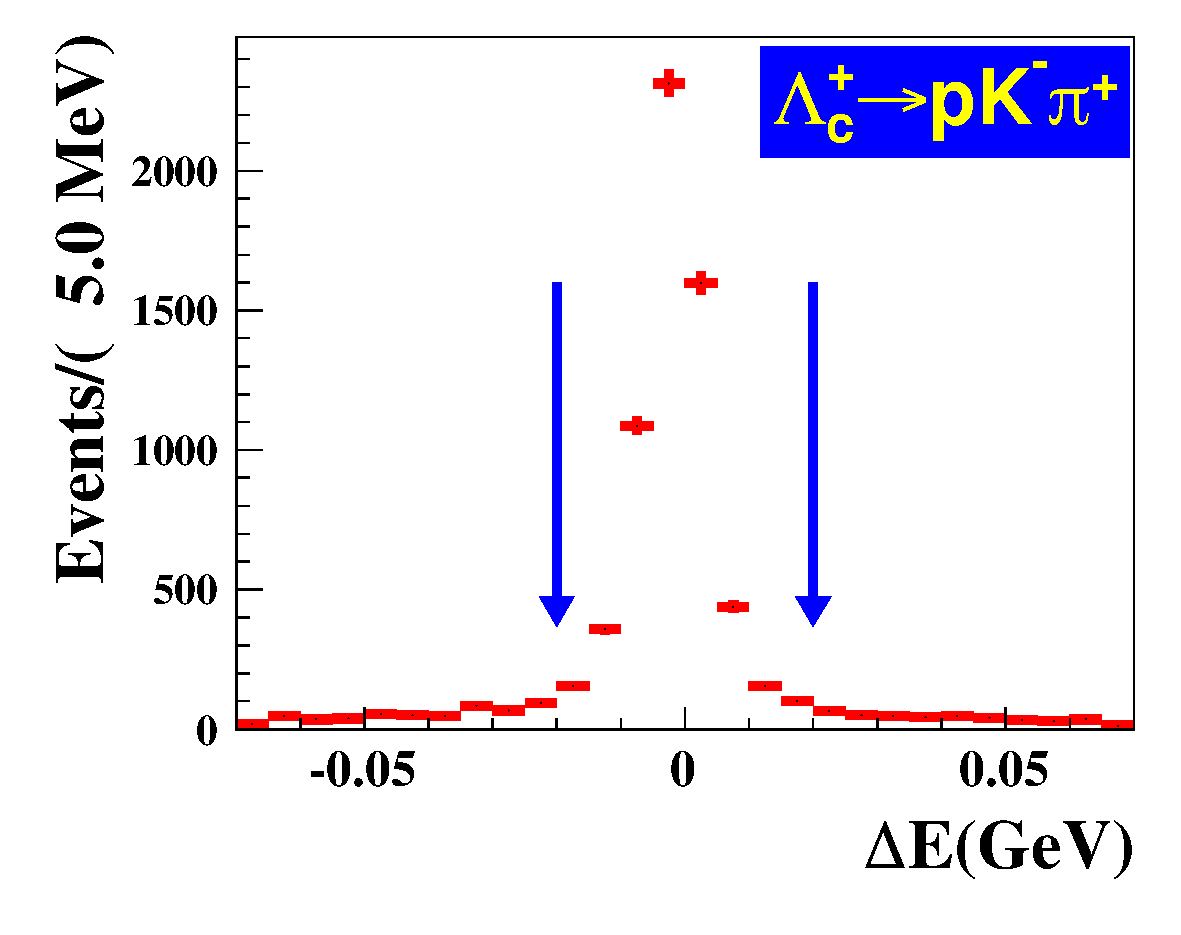
\includegraphics[width=0.4\textwidth]{chap2_data_deltaE_mode1}
}
\subfigure[]
{
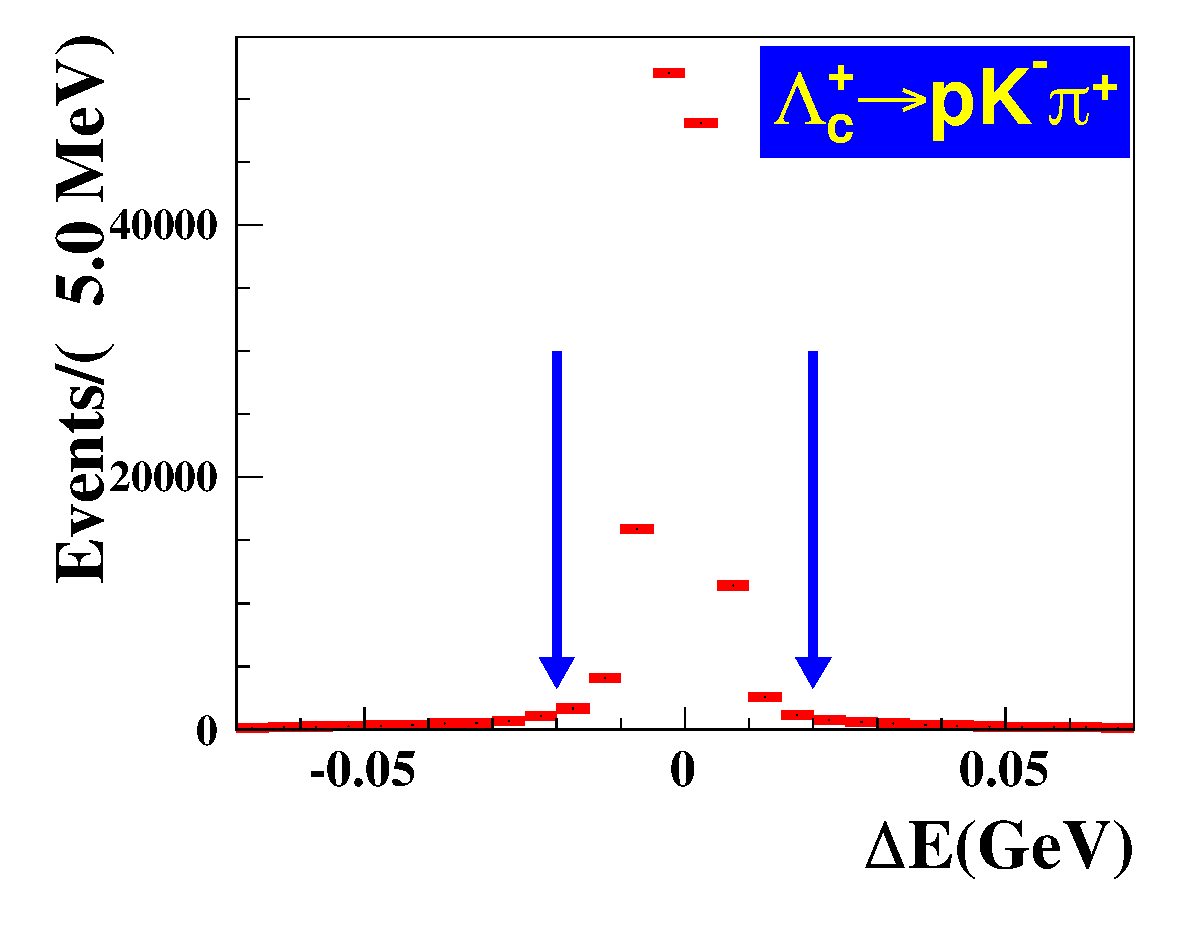
\includegraphics[width=0.4\textwidth]{chap2_sigmc_deltaE_mode1}
}
\caption{$\Lmodeb$衰变中$\Delta{}E$的分布,左图为数据中的分布,右图为单标记信号MC的分布。图中箭头指示了信号区间。}
\label{fig:deltaE}
\end{figure*}


%%%%%%%%%%%%%%%%%%%%%%%%%%%%%%%%%%%%%%%
\begin{table}[H]
  \begin{center}
  %\footnotesize
 \caption{单标记$\lambdacp$的$\Delta{}E$要求, 单标记产额$N_{i}^{\rm ST}$以及单标记$\varepsilon_{i}^{\rm ST}$。 双标记效率$\varepsilon_{i,\Xi K}^{\rm DT}$ 和双标记效率$\varepsilon_{i,\Xi^{*}K}^{\rm DT}$。误差只包含统计误差。效率不包含任何中间共振态的分支比$\mathcal{B}$。}
  \resizebox{\linewidth}{!}{
  \begin{tabular}{l|c|c|c|c|c}
      \hline \hline
  衰变道  &$\Delta{}E$ (MeV) & $N_{i}^{\rm ST}$ & $\varepsilon_{i}^{\rm ST}(\%)$ & $\varepsilon_{i,\Xi K}^{\rm DT}(\%)$  & $\varepsilon_{i,\Xi^{*}K}^{\rm DT}(\%)$\\ \hline
$\textbf{$\modea$}$ & $(-20,20)$ & $1145\pm34$ & $51.6$ & $41.2$ & $42.6$  \\
$\textbf{$\modeb$}$ & $(-20,20)$ & $5722\pm80$ & $45.2$ & $37.3$ & $39.1$ \\
$\textbf{$\modec$}$ & $(-30,20)$ & $478\pm28$ & $17.2$ & $15.1$ & $15.2$ \\
$\textbf{$\moded$}$ & $(-20,20)$ & $431\pm25$ & $18.6$ & $15.4$ & $15.2$ \\
$\textbf{$\modee$}$ & $(-30,20)$ & $1407\pm51$ & $14.7$ & $13.4$ & $12.7$ \\
$\textbf{$\modef$}$ & $(-20,20)$ & $474\pm41$ & $55.4$ & $43.3$ & $45.1$ \\
$\textbf{$\modeaa$}$ & $(-20,20)$ & $648\pm25$ & $38.7$ & $30.9$ & $31.4$ \\
$\textbf{$\modebb$}$ & $(-30,20)$ & $1282\pm43$ & $13.0$ & $10.9$ & $11.2$ \\
$\textbf{$\modedd$}$ & $(-20,20)$ & $540\pm27$ & $10.6$ & $9.0$ & $8.8$ \\
$\textbf{$\modeaaa$}$ & $(-20,20)$ & $427\pm23$ & $24.1$ & $20.6$ & $20.6$ \\
$\textbf{$\modeccc$}$ & $(-50,30)$ & $258\pm20$ & $19.6$ & $17.3$ & $17.4$ \\
$\textbf{$\modeddd$}$ & $(-30,20)$ & $1005\pm42$ & $20.1$ & $17.2$ & $18.1$ \\ 
\hline  \hline
   \end{tabular}
   }
   \label{tab:STyields}
  \end{center}
  \end{table}


%%%%%%%%%%%%%%%%%%%%%%%%%%%%%%
\section{本底检查}
选择好事例后,通过拟合$M_{\rm BC}$的分布可以提取信号个数。在这之前,先用单举的MC样本(Inclusive MC)来查看每一个单标记道的本底情况。
我们发现有一些衰变道遭受着来自具有相同末态的其他衰变道的污染,贡献为所谓的峰本底。
为了去掉这些本底,我们根据本底道的过程引进了一些本底道的特征变量,然后设置窗口从而将这些本底去掉。
具体的窗口要求列在表~\ref{tab:bkg}中。在单标记和双标记的时候都采用了这一去本底的窗口要求。
\begin{table}
  \begin{center}
  \footnotesize
   \caption{$\lambdacp$具有峰本底的衰变道和对应的本底过程及其去除方法。}
  \begin{tabular}{l|c|c}
      \hline \hline
       衰变道  & 本底过程& 去本底的方法 \\ \hline
       \multirow{2}{*}{$\modec$} & $\modebb$ & 要求$M(p\pim)$不在 $\Lambda$质量区间 $(1.11,1.12)\gevcc$内\\ \cline{2-3}
       & $\Sigma^+\pip\pim$ & 要求$M(p\pizero)$不在$\Sigmap$质量区间 $(1.17,1.2)\gevcc$内 \\ \hline
       $\moded$ & $\modedd$ & 要求$M(p\pim)$不在$\Lambda$质量区间 $(1.11,1.12)\gevcc$内 \\ \hline
       $\modedd$ & $\moded$ & 要求$M(\pip\pim)$不在$\Ks$质量区间$(0.48,0.52)\gevcc$内 \\ \hline
       $\modeccc$ & $\modea$ & 要求$M(\pizero\pizero)$不在$\Ks$质量区间$(0.48,0.52)\gevcc$内 \\ \hline
       \multirow{2}{*}{$\modeddd$} & $\modec$ &要求$M(\pip\pim)$不在$\Ks$质量区间$(0.48,0.52)\gevcc$内 \\ \cline{2-3}
       & $\modebb$ &  要求$M(p\pim)$不在 $\Lambda$质量区间$(1.11,1.12)\gevcc$内 \\ \cline{2-3}
    \hline\hline
   \end{tabular}
   \label{tab:bkg}
  \end{center}
  \end{table}
当采用了这一措施之后,我们可以看出已经没有了峰本底的影响。
图~\ref{fig:compare_dataMC}给出了Cocktail MC和数据的比较图,我们可以看到两者吻合的非常好。
此外,我们还定量地检查了cross feed过程影响。所谓的 cross feed 指的是这12个衰变道之间,其余11个衰变道对该信号道的污染情况。
我们定义两个变量:cross feed几率和cross feed数目比例,顾名思义,cross feed几率指的是11个本底衰变道被当作该信号道选进来的几率;
而cross feed数目指的是数据中11个本底衰变道被当作该信号道选进来的绝对的数目。
这两个量是严格相关的,cross feed数目取决于cross feed几率以及数据中该本底道的数目,我们按照我们测量的分支比以及cross feed几率来计算的cross feed数目,进一步的计算cross feed数目占该过程产额的比例。
这两个量都是有意义的,原则上cross feed数目比例是更有直接的参考意义的。
讲这些值和产额的统计误差比起来,我们可以看出峰本底已经被压低到了完全可以忽略的地步。

%%%%%%%%%%%%%%%%%%%%%%%%%%%%
\begin{figure*}[hp]
\centering
\subfigure[]
{
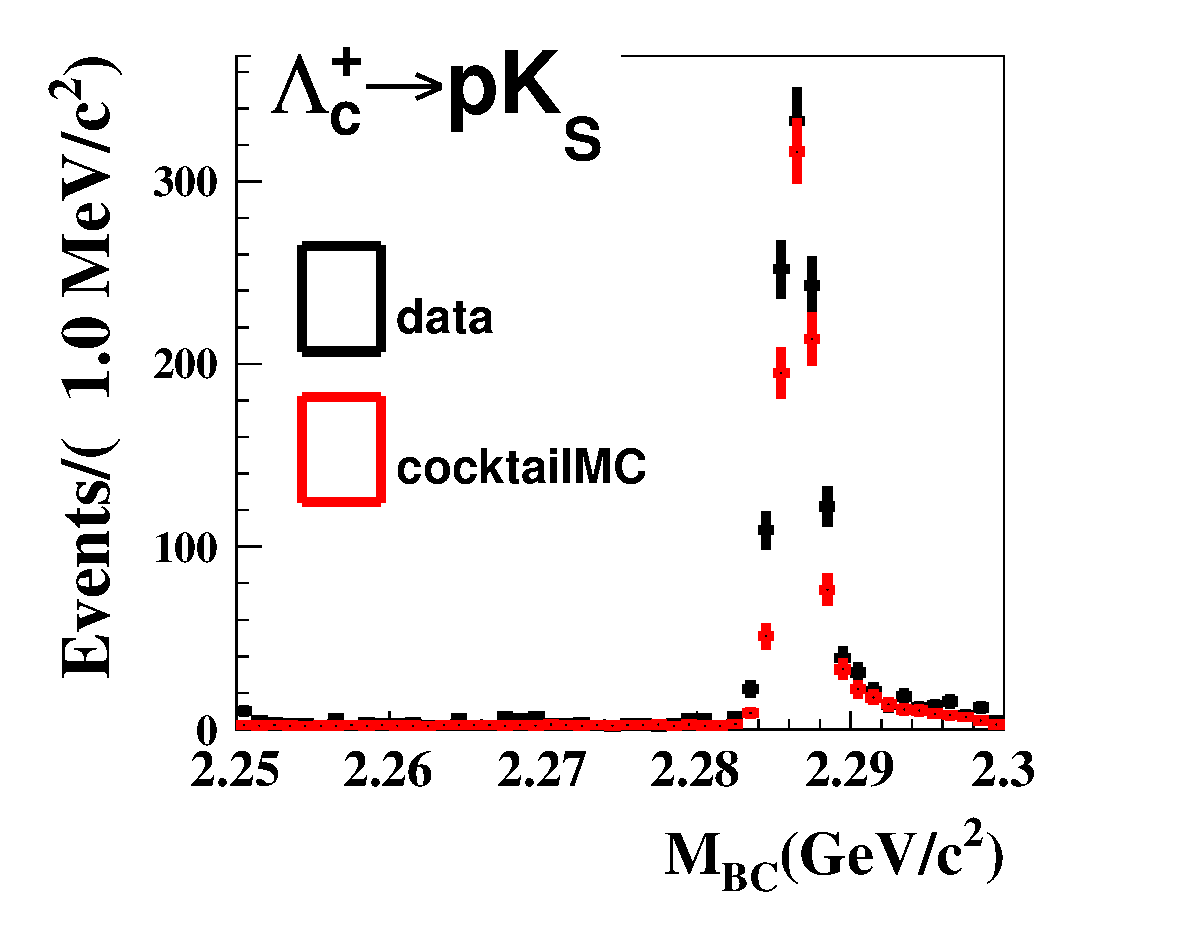
\includegraphics[width=0.3\textwidth]{chap2_compare_mode0}
}
\hspace{1pt}
\subfigure[]
{
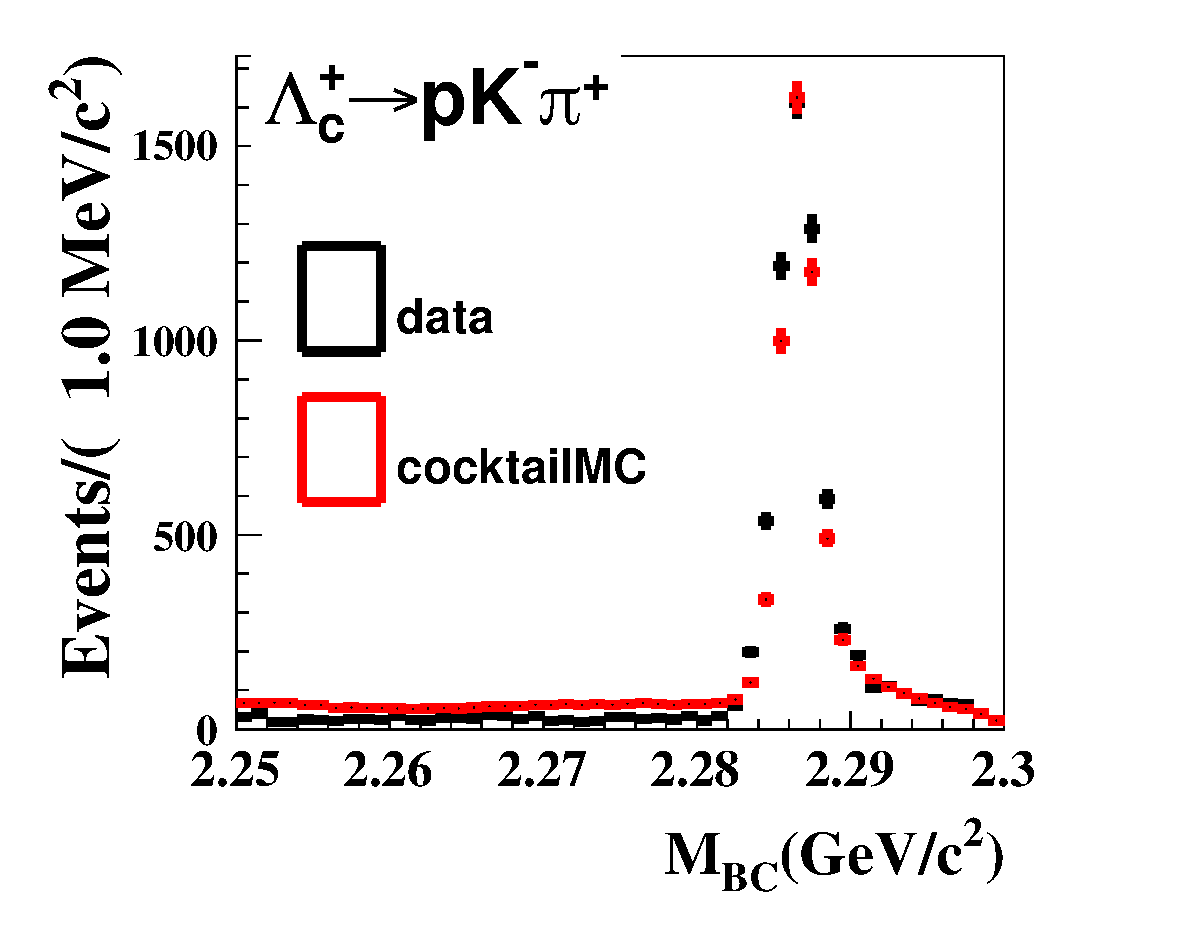
\includegraphics[width=0.3\textwidth]{chap2_compare_mode1}
}
\hspace{1pt}
\subfigure[]
{
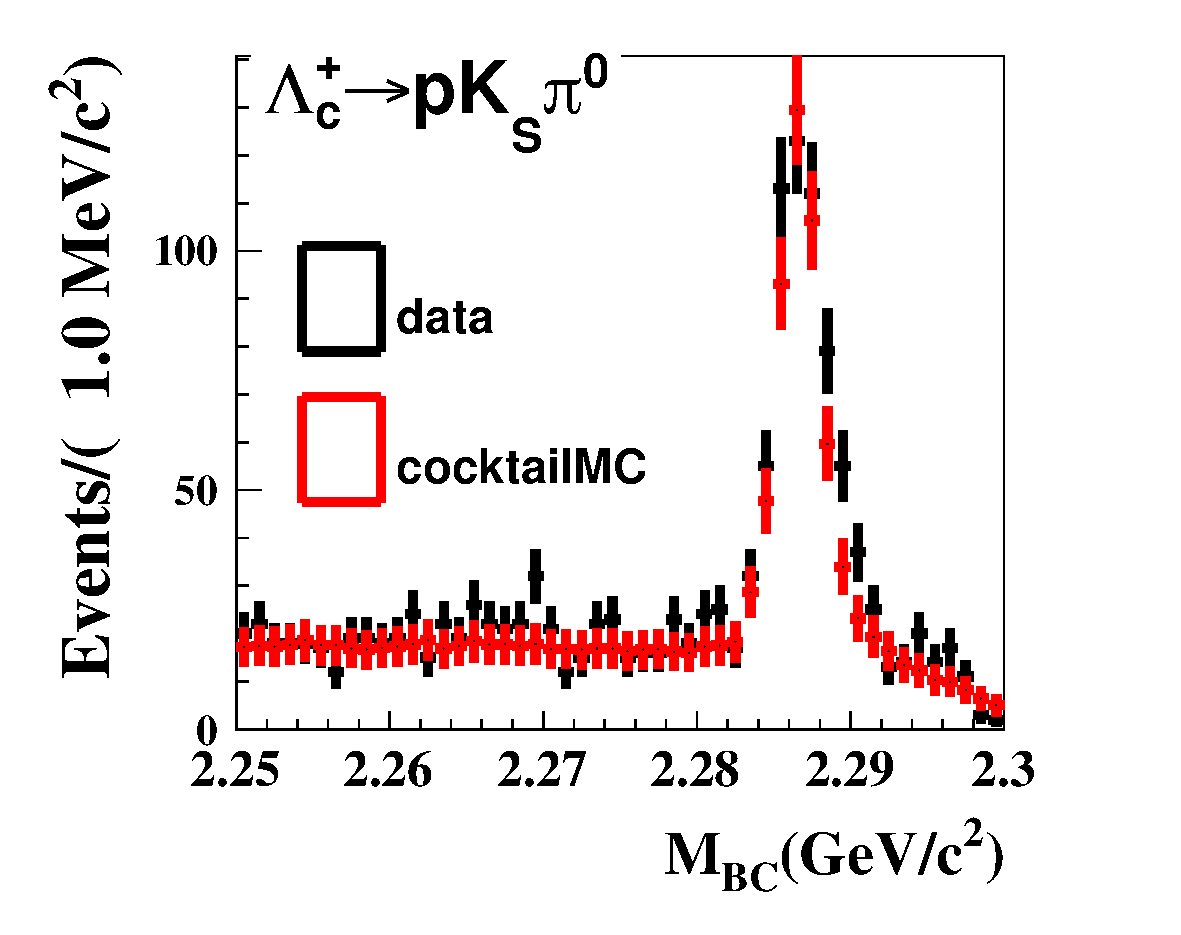
\includegraphics[width=0.3\textwidth]{chap2_compare_mode2}
}
\hspace{1pt}
\subfigure[]
{
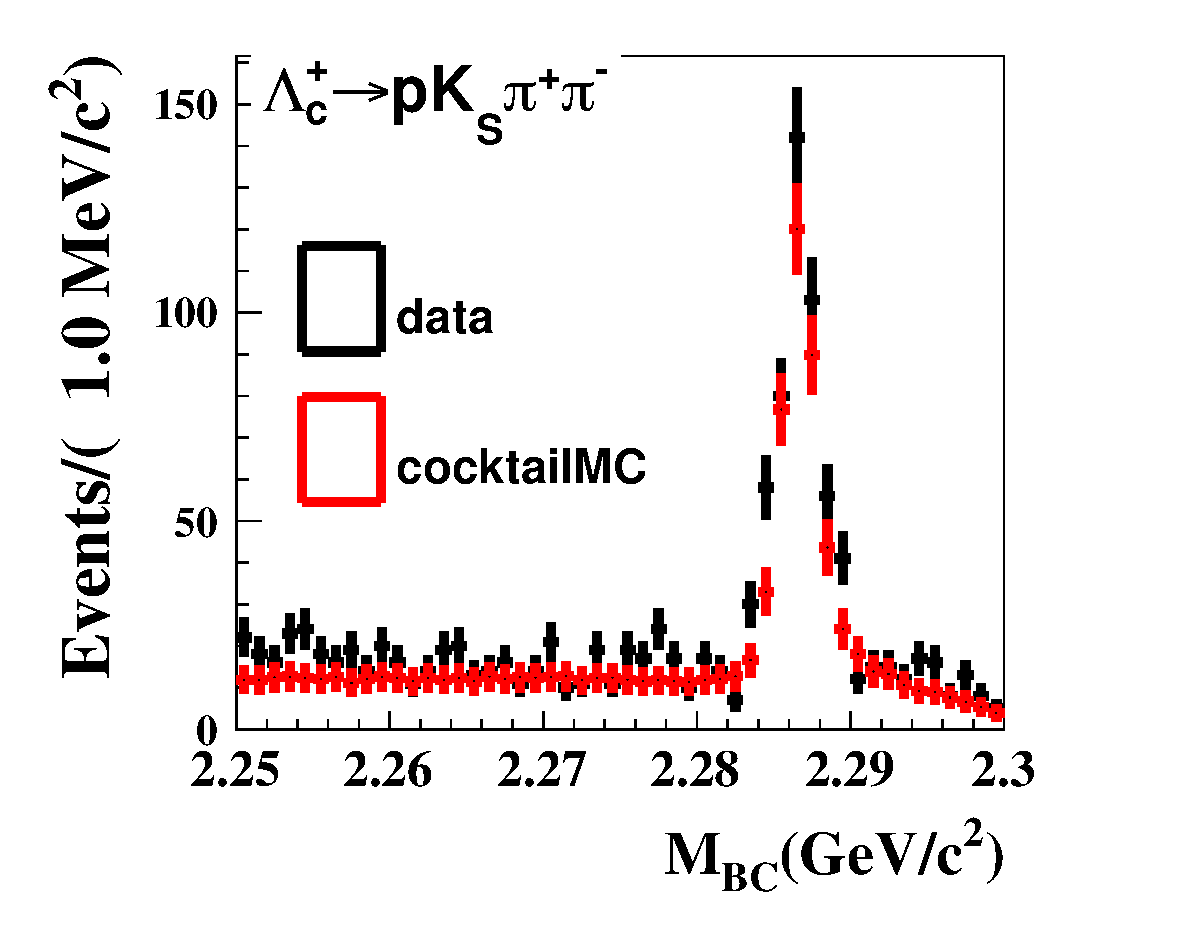
\includegraphics[width=0.3\textwidth]{chap2_compare_mode3}
}
\hspace{1pt}
\subfigure[]
{
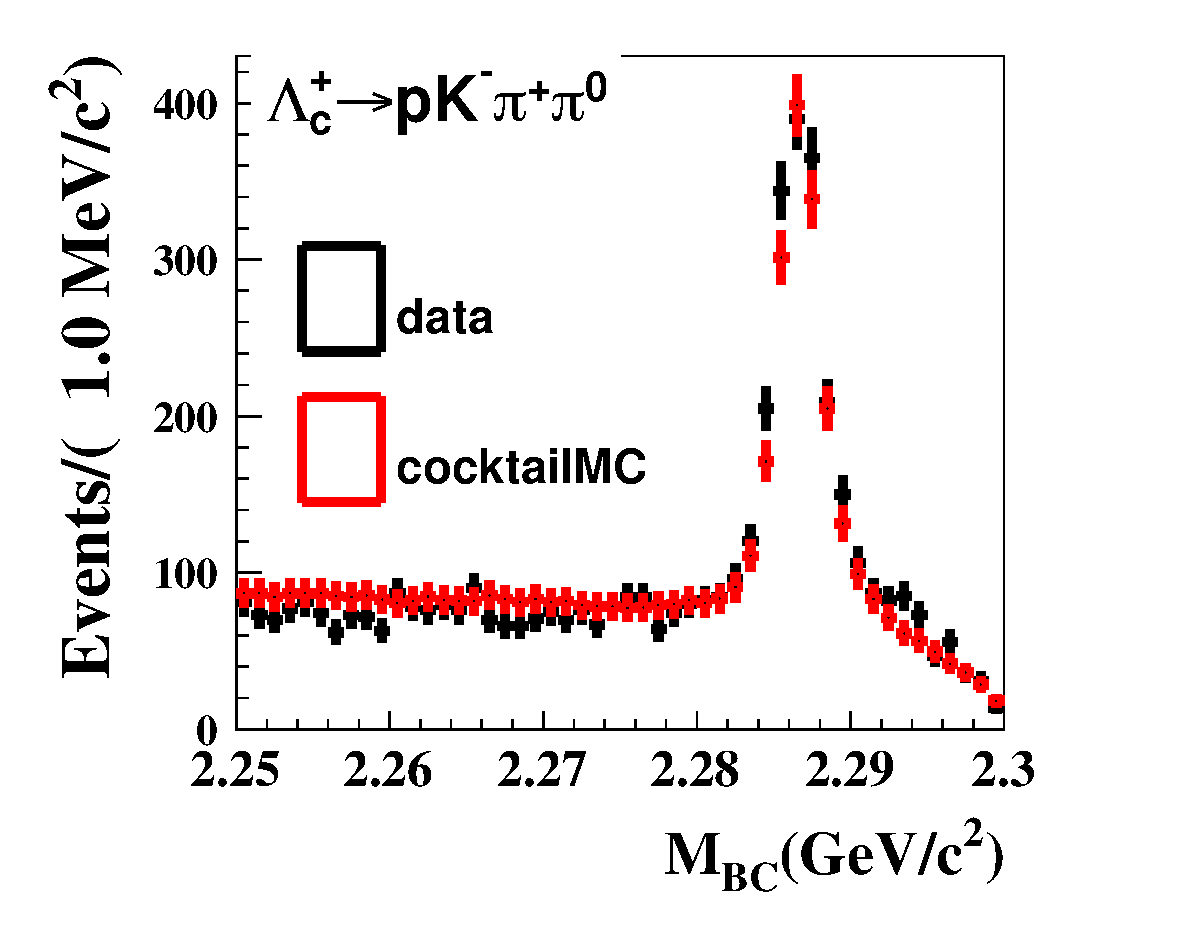
\includegraphics[width=0.3\textwidth]{chap2_compare_mode4}
}
\hspace{1pt}
\subfigure[]
{
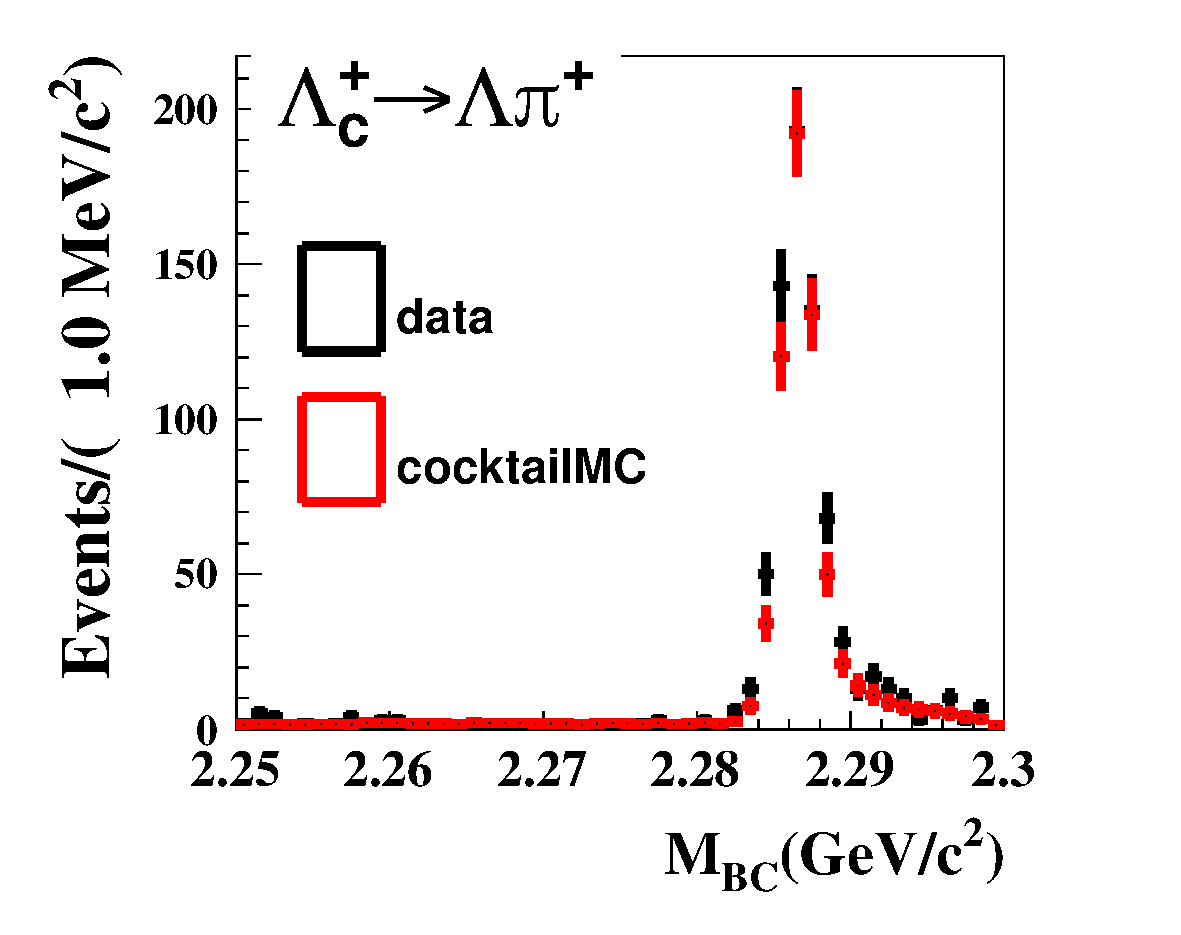
\includegraphics[width=0.3\textwidth]{chap2_compare_mode30}
}
\hspace{1pt}
\subfigure[]
{
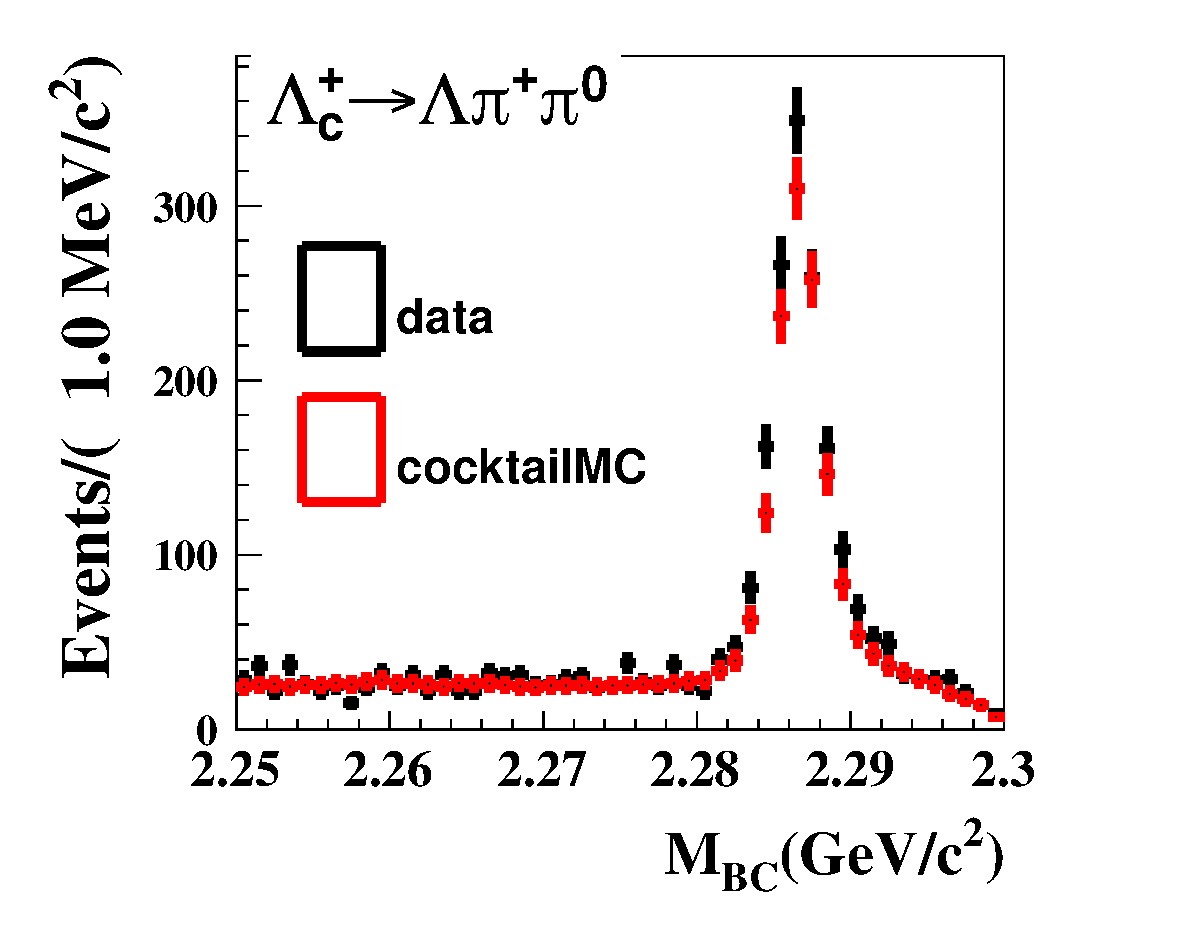
\includegraphics[width=0.3\textwidth]{chap2_compare_mode31}
}
\hspace{1pt}
\subfigure[]
{
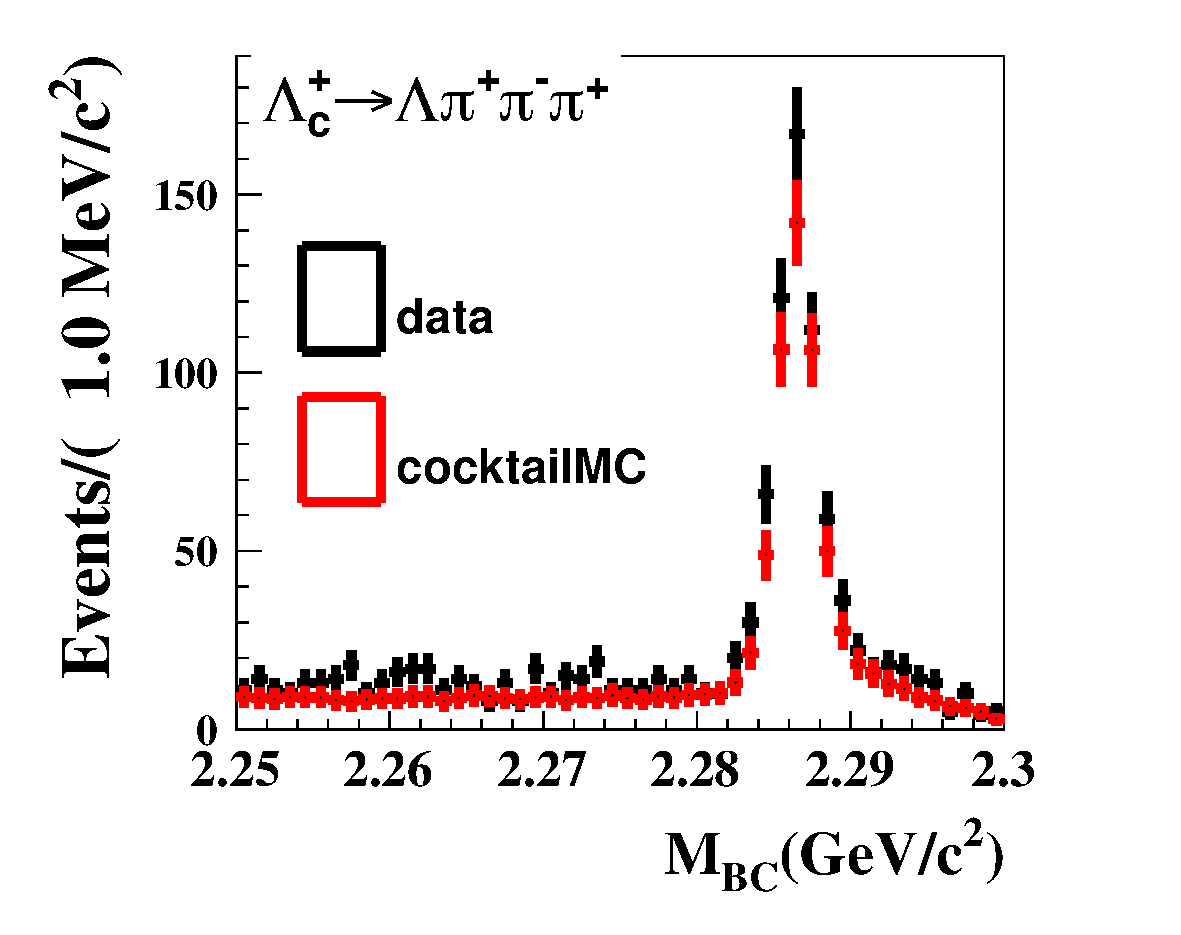
\includegraphics[width=0.3\textwidth]{chap2_compare_mode33}
}
\hspace{1pt}
\subfigure[]
{
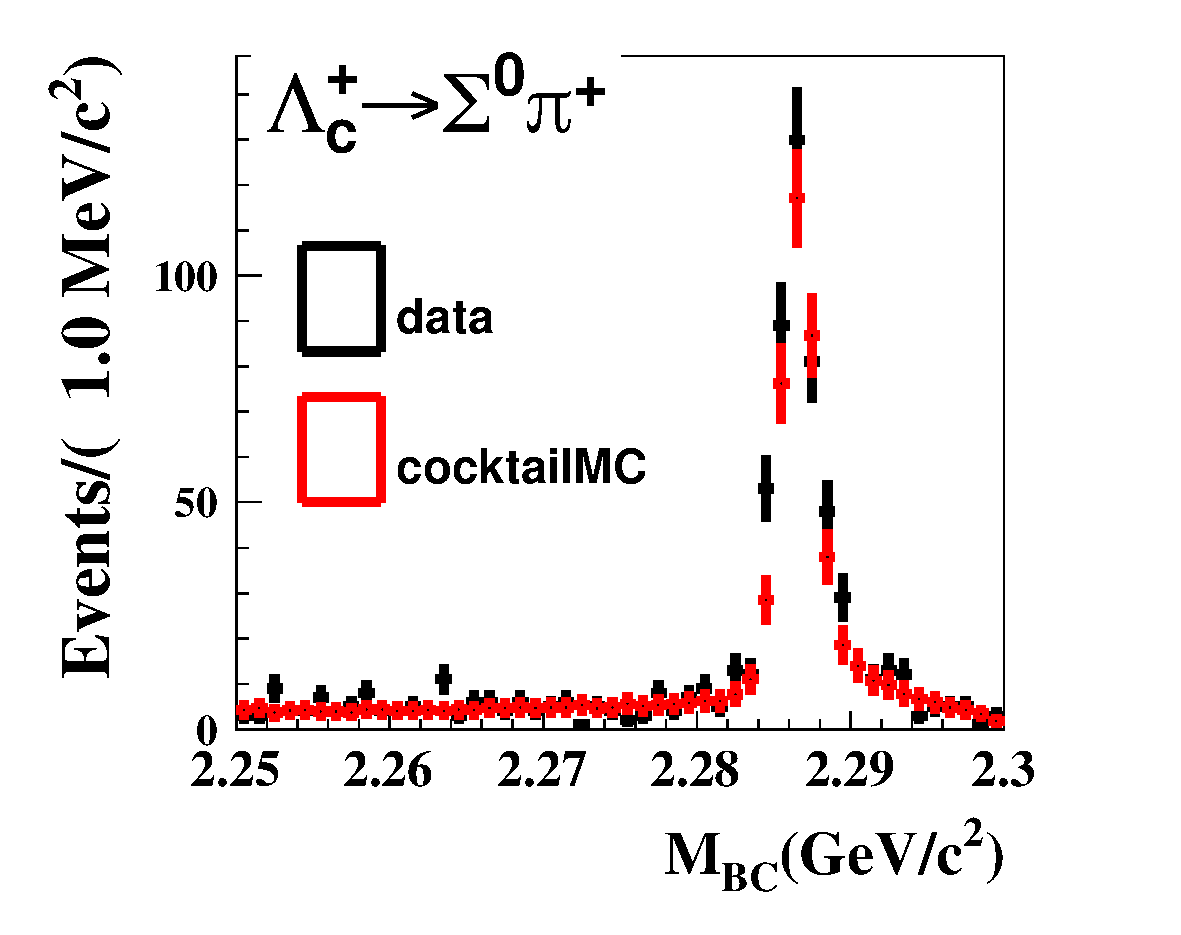
\includegraphics[width=0.3\textwidth]{chap2_compare_mode60}
}
\hspace{1pt}
\subfigure[]
{
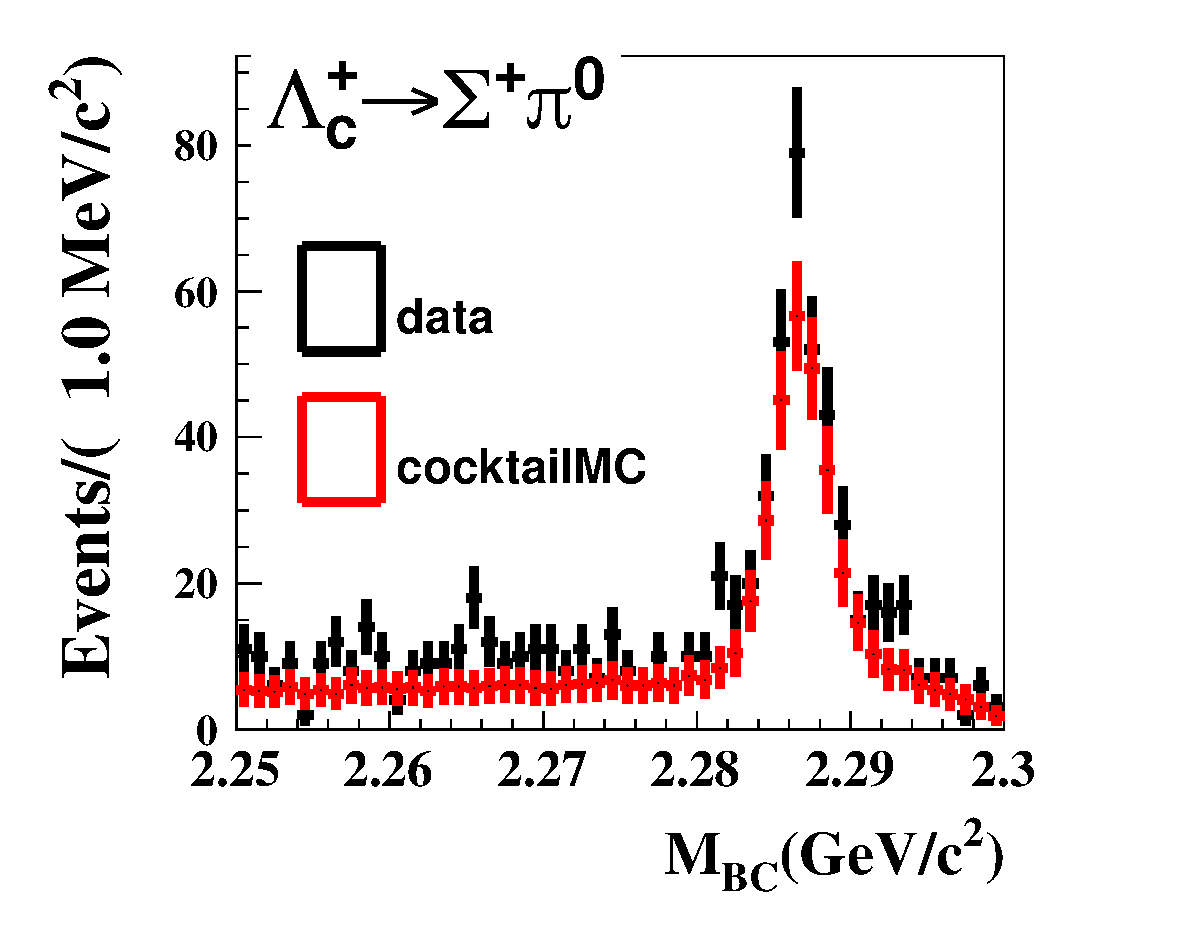
\includegraphics[width=0.3\textwidth]{chap2_compare_mode62}
}
\hspace{1pt}
\subfigure[]
{
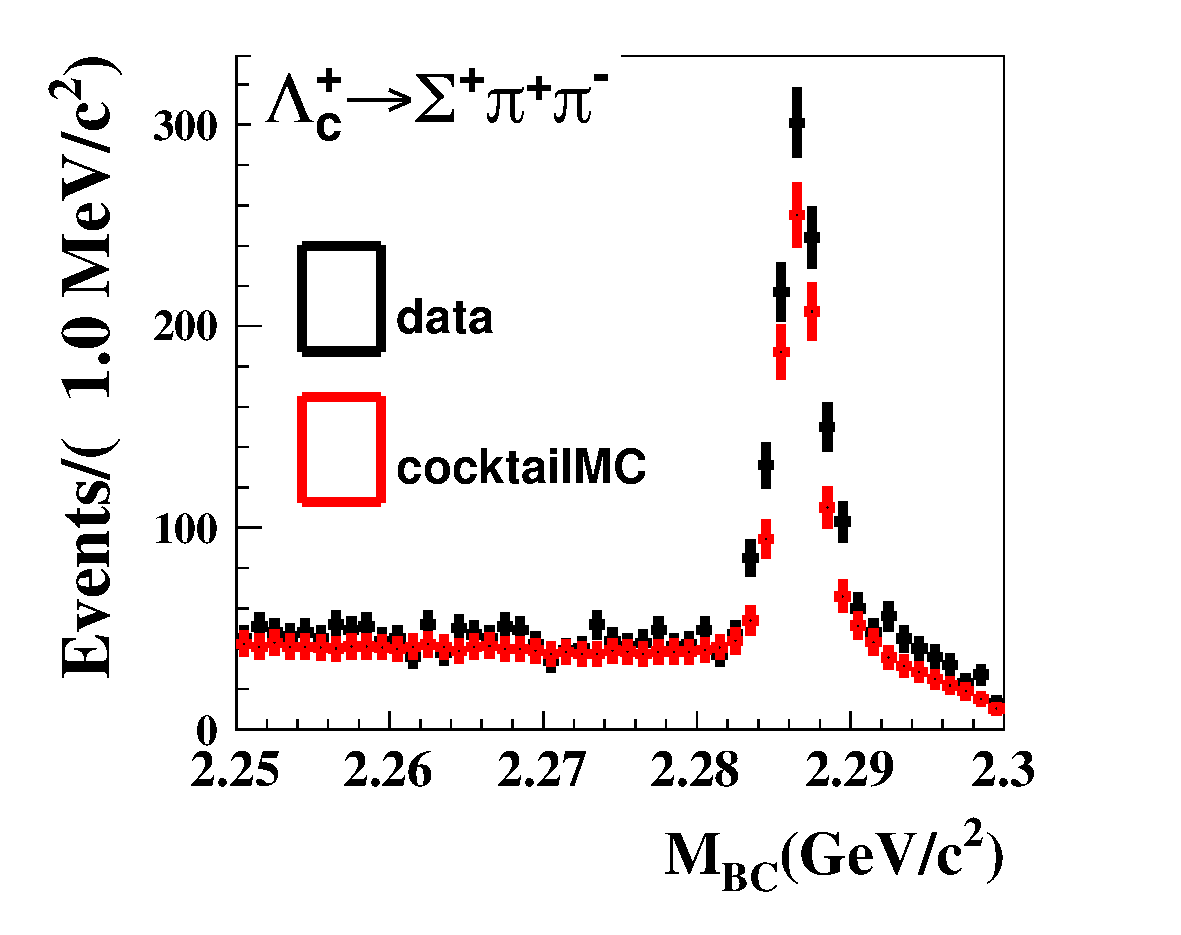
\includegraphics[width=0.3\textwidth]{chap2_compare_mode63}
}
\hspace{1pt}
\subfigure[]
{
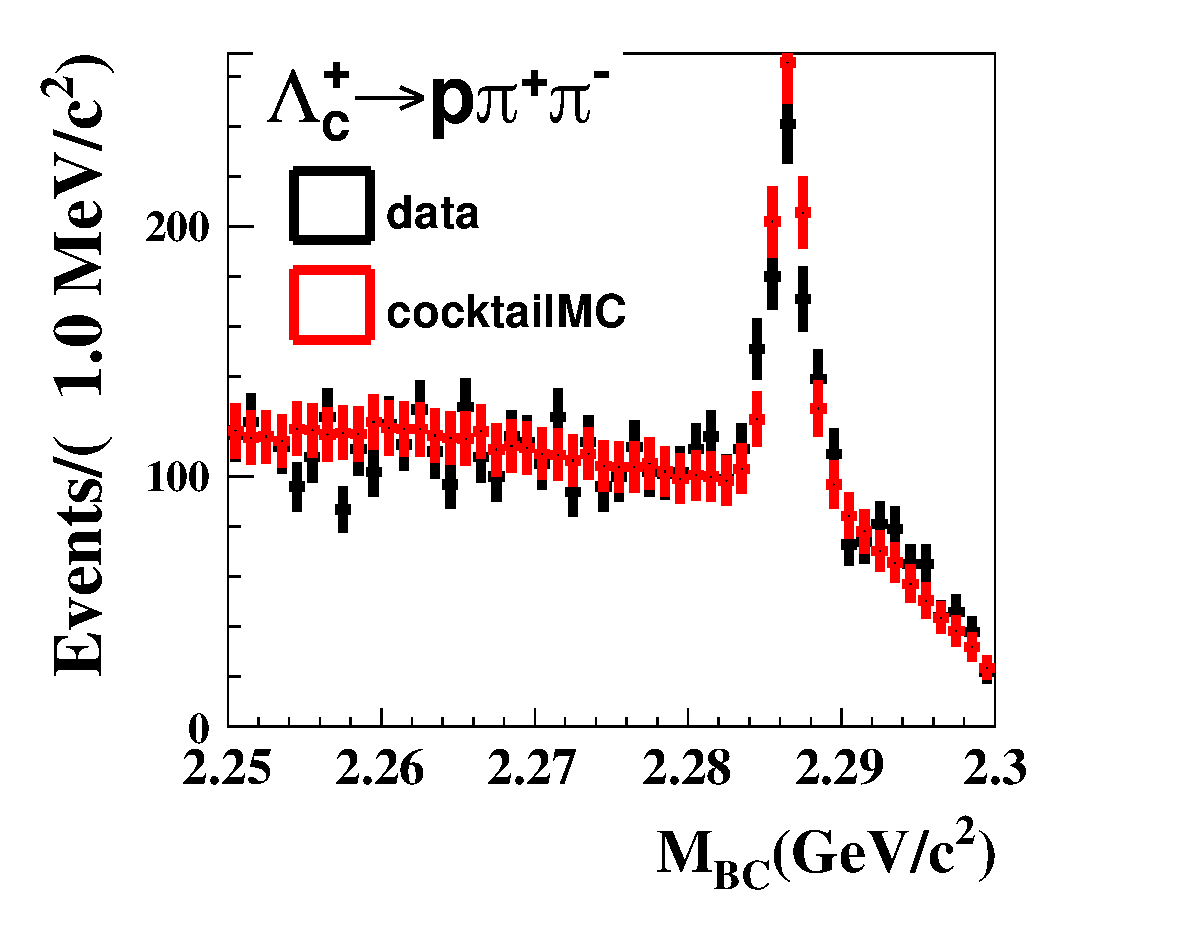
\includegraphics[width=0.3\textwidth]{chap2_compare_mode5}
}
\caption{Cocktail MC和数据的比较图。}
\label{fig:compare_dataMC}
\end{figure*}

\section{单标记数据分析}
对于单标记一侧的分析,如果在重建一个$\lambdacpm$ 的衰变道过程中有了多个候选者,我们选择一个具有最小的$|\Delta{}E|$的候选者保留下来。
当我们通过初步的事例筛选,且对$\Delta{}E$做了相应要求,每一个衰变道拿到了相应的候选事例,然后我们通过拟合$M_{\rm BC}$的分布来提取信号和本底的数目。
我们对于数据和MC采用的拟合方法均为不分区间的极大似然拟合。
把产额和效率作为待测参数通过拟合来提取。
图~\ref{fig:ST_datafit}给出了数据中每个道的拟合结果,我们是把电荷共轭道的$\lambdacp$和$\lambdacm$合并在一起来进行估计的。
拟合区间为~[2.25,2.3]$\gevcc$。 
在每一个道的拟合函数中都包含着两部分,信号形状和本底形状。
图中黑色的带误差的点是数据,红线是总的拟合线,绿色的虚线是信号的形状,蓝色的虚线是用来描述本底的ARGUS函数~\cite{ref:argus}。
信号形状我们采用来自于单标记的信号形状MC卷积一个高斯函数来描述。
高斯函数用于描述由于束流能量($E_{\rm beam}$)测量不够准确给~$M_{\rm BC}$ 带来的偏移以及~MC 和数据的分辨差异,其中心值和宽度都是浮动的。
ARGUS本底函数的具体表达式为:
\begin{equation}
f(m;m_{0},\xi)=Am(1-\frac{m^{2}}{m^{2}_{0}})^{0.5} e^{\xi(1-\frac{m^{2}}{m_{0}^{2}})}.
\end{equation}
其中,$A$ 是归一化系数;$m$ 是要拟合的量(即~$M_{\rm BC}$);$m_{0}$ 是右端的截断值,对于~$M_{\rm BC}$ 而言,其右端的截断值应该等于~$e^{+}e^{-}$ 束流的平均能量~$E_{\rm beam}$,在拟合时我们将~$m_{0}$ 固定为$2.3$;$\xi$ 是另一个浮动参数,通过拟合获得。
我们抽取$M_{\rm BC}$在$(2.282, 2.291)\gevcc$之间的事例产额作为该衰变道单标记的事例数$N_{i}^{ST}$。

为了获取单标记侧信号过程的筛选效率,也同时考虑到要降低系统误差的需求,我们在对MC拟合之前先考虑了MC样本和数据样本在$\Delta E$和$M_{\rm BC}$谱分辨上的差异。
利用图~\ref{fig:ST_datafit}拟合$M_{\rm BC}$谱过程中给出来的高斯分辨参数我们可以知道现有MC样本和数据样本之间在分辨上的差异。
为了拿到在$\Delta E$谱上MC和数据在分辨上的差异,我们对数据中$\Delta E$的分布也进行了拟合。

在拿到$\Delta E$和$M_{\rm BC}$谱上MC数据之间的分辨函数之后,我们按照这一参数对现有MC的$\Delta E$和$M_{\rm BC}$谱进行修正,使其分辨和数据尽可能的一致。
所谓的修正就是按照拟合得到的分辨函数去弥散原始MC的分布。
用这份修正过的MC样本加上Cocktail MC中的其他过程,生成一份新的Cocktail MC。
然后利用和数据完全类似的拟合方法来拟合这份新的Cocktail MC样本来得到单标记的选择效率。
图~\ref{fig:ST_cockmcfit}是拟合结果图。MC的拟合依然是合并了$\lambdacp$和$\lambdacm$的衰变的。
我们将具体的单标记产额值和效率值列在表~\ref{tab:STyields}中。
分别对应公式\ref{eq:st}中的$N_{i}^{ST}$和$\varepsilon_{i}^{ST}$。
这些效率值是不包含表~\ref{tab:interDecay}中的次级衰变分支比的。

%%%%%%%%%%%%%%%%%%%%%%%%%%%%%%%%%%%%%%%%%%%%%%%%%%%%%%%%%%%%%%%%%%%%%%%%%%%%%%%%%%%%%%%%%
\begin{figure*}[]
\centering
\subfigure[]
{
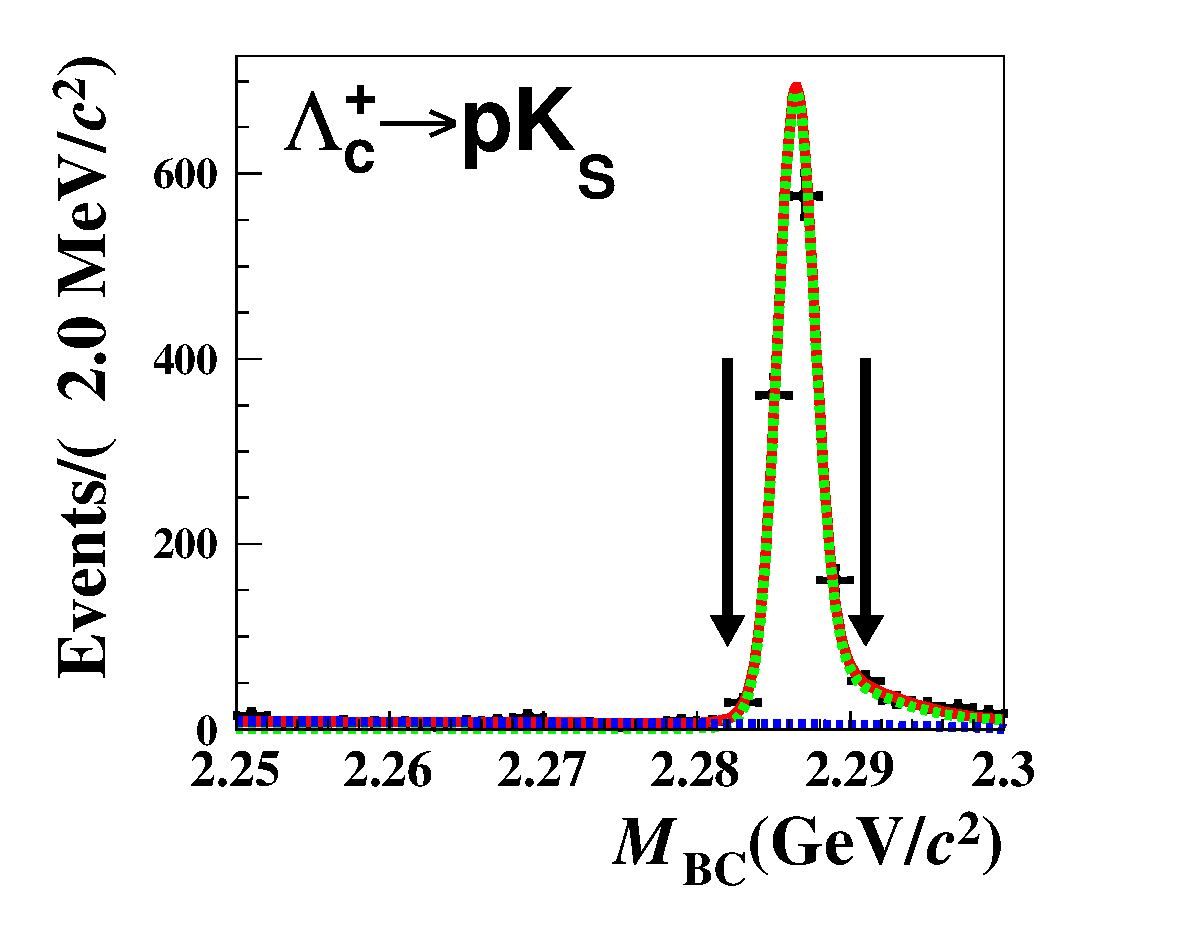
\includegraphics[width=0.3\textwidth]{chap2_ST_data_mode0}
}
\hspace{1pt}
\subfigure[]
{
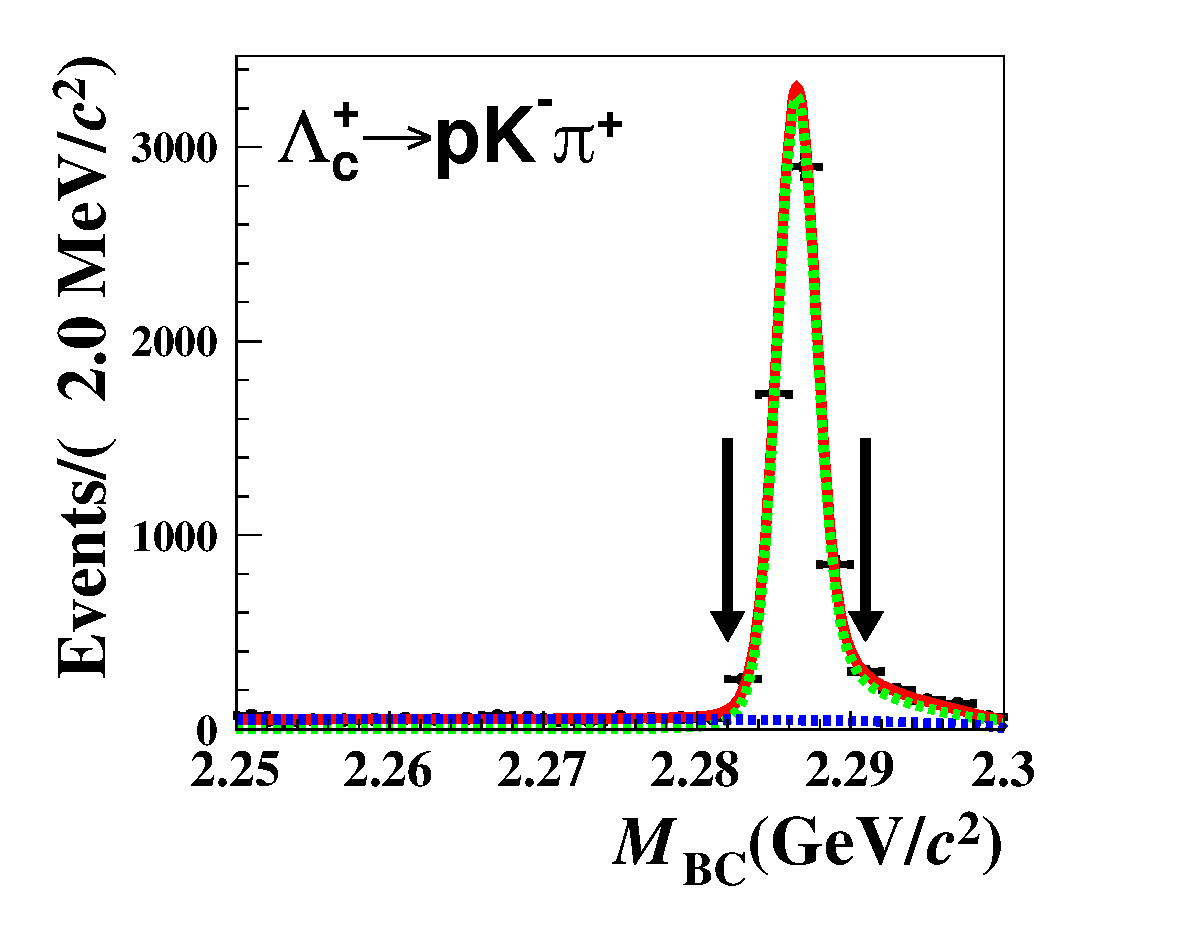
\includegraphics[width=0.3\textwidth]{chap2_ST_data_mode1}
}
\hspace{1pt}
\subfigure[]
{
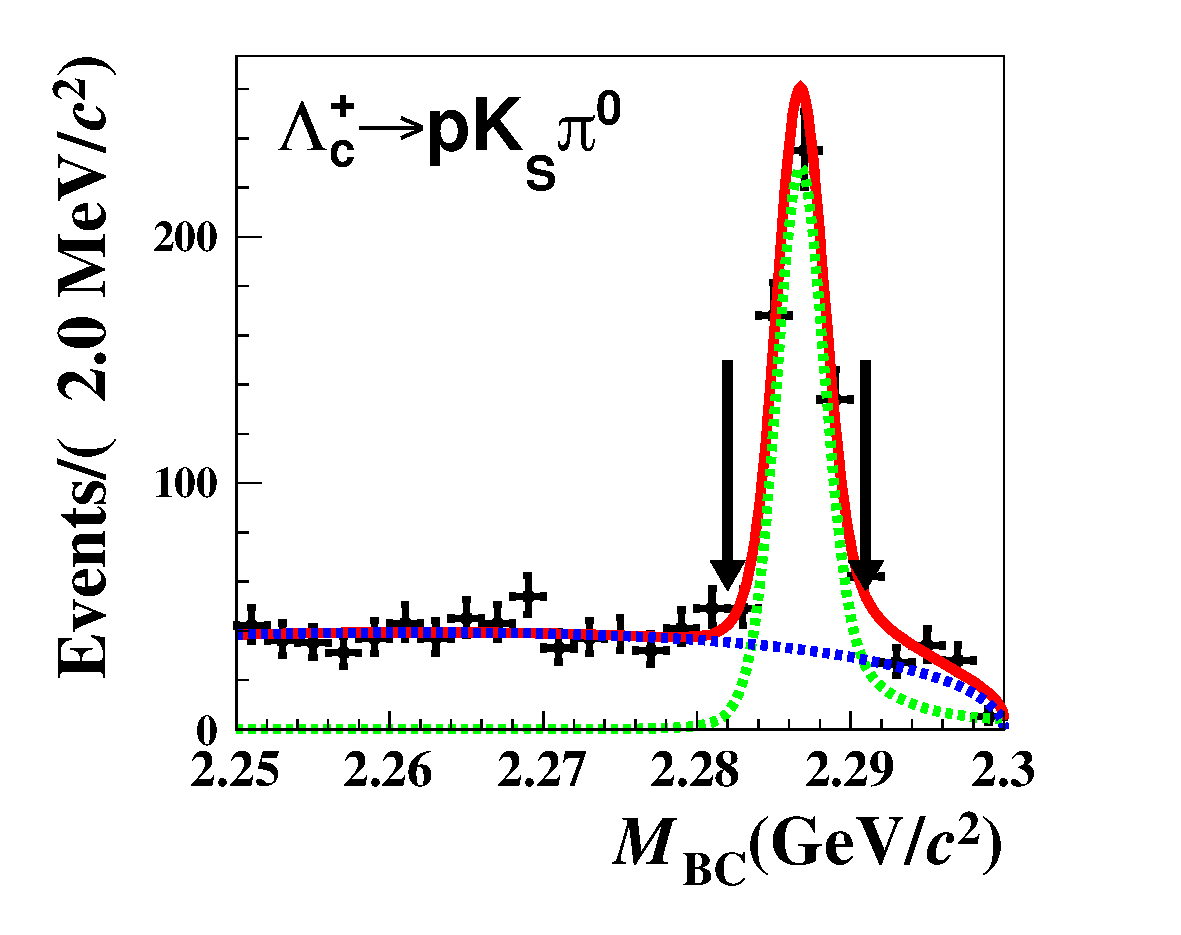
\includegraphics[width=0.3\textwidth]{chap2_ST_data_mode2}
}
\hspace{1pt}
\subfigure[]
{
\includegraphics[width=0.3\textwidth]{chap2_ST_data_mode3}
}
\hspace{1pt}
\subfigure[]
{
\includegraphics[width=0.3\textwidth]{chap2_ST_data_mode4}
}
\hspace{1pt}
\subfigure[]
{
\includegraphics[width=0.3\textwidth]{chap2_ST_data_mode30}
}
\hspace{1pt}
\subfigure[]
{
\includegraphics[width=0.3\textwidth]{chap2_ST_data_mode31}
}
\hspace{2pt}
\subfigure[]
{
\includegraphics[width=0.3\textwidth]{chap2_ST_data_mode33}
}
\hspace{1pt}
\subfigure[]
{
\includegraphics[width=0.3\textwidth]{chap2_ST_data_mode60}
}
\hspace{1pt}
\subfigure[]
{
\includegraphics[width=0.3\textwidth]{chap2_ST_data_mode62}
}
\hspace{1pt}
\subfigure[]
{
\includegraphics[width=0.3\textwidth]{chap2_ST_data_mode63}
}
\hspace{1pt}
\subfigure[]
{
\includegraphics[width=0.3\textwidth]{chap2_ST_data_mode5}
}
\caption{拟合\textbf{数据}中单标记~$M_{\rm BC}$分布得产额的拟合结果,每个道的~$\lambdacp$ 及~$\lambdacm$ 均合在一起拟合。在每个图中,黑色的带误差的点代表数据的分布,红色实的曲线是拟合结果,绿色虚线是信号的形状,蓝色虚线是本底ARGUS函数分布。}
\label{fig:ST_datafit}
\end{figure*}


%%%%%%%%%%%%%%%%%%%%%%%%%%%%
\begin{figure*}[]
\centering
\subfigure[]
{
\includegraphics[width=0.3\textwidth]{chap2_ST_cockmc_mode0}
}
\hspace{1pt}
\subfigure[]
{
\includegraphics[width=0.3\textwidth]{chap2_ST_cockmc_mode1}
}
\hspace{1pt}
\subfigure[]
{
\includegraphics[width=0.3\textwidth]{chap2_ST_cockmc_mode2}
}
\hspace{1pt}
\subfigure[]
{
\includegraphics[width=0.3\textwidth]{chap2_ST_cockmc_mode3}
}
\hspace{1pt}
\subfigure[]
{
\includegraphics[width=0.3\textwidth]{chap2_ST_cockmc_mode4}
}
\hspace{1pt}
\subfigure[]
{
\includegraphics[width=0.3\textwidth]{chap2_ST_cockmc_mode30}
}
\hspace{1pt}
\subfigure[]
{
\includegraphics[width=0.3\textwidth]{chap2_ST_cockmc_mode31}
}
\hspace{1pt}
\subfigure[]
{
\includegraphics[width=0.3\textwidth]{chap2_ST_cockmc_mode33}
}
\hspace{1pt}
\subfigure[]
{
\includegraphics[width=0.3\textwidth]{chap2_ST_cockmc_mode60}
}
\hspace{1pt}
\subfigure[]
{
\includegraphics[width=0.3\textwidth]{chap2_ST_cockmc_mode62}
}
\hspace{1pt}
\subfigure[]
{
\includegraphics[width=0.3\textwidth]{chap2_ST_cockmc_mode63}
}
\hspace{1pt}
\subfigure[]
{
\includegraphics[width=0.3\textwidth]{chap2_ST_cockmc_mode5}
}
\caption{拟合\textbf{Cocktail MC}中单标记~$M_{\rm BC}$分布得重建效率的拟合结果,每个道的~$\lambdacp$ 及~$\lambdacm$ 均合在一起拟合。在每个图中,黑色的带误差的点代表数据样本的分布,红色实的曲线是拟合结果,蓝色虚线是本底ARGUS函数分布。}

\label{fig:ST_cockmcfit}
\end{figure*}



\section{双标记侧寻找$\LtoXiK$~和~$\LtoXisK$}
为了获取双标记事例,我们在先重建一个单侧$\lambdacp$($\lambdacm$)的基础上,再在剩余的径迹中去寻找另外一个$\lambdacm$($\lambdacp$)的候选事例。
为了得到$\LtoXiK$~和~$\LtoXisK$的候选态,
我们要求单标记侧的$\lambdacp$($\lambdacm$)的$M_{\rm BC}$应该落在信号区$(2.282,2.291)\gevcc$内。
同时我们再找一条额外的带电径迹($\Xi^{0}$和$\Xi{(1530)}^{0}$不去重建),其电荷号应该要与标记侧$\Lambda_c$的电荷号相反。
接下来我们要求这条带电径迹应该满足$K$介子的粒子鉴别条件,详情如下:
 \begin{itemize}
 \item $|\delta r|<1\,\unit{cm}$, $|\delta z|<10\,\unit{cm}$, $|\cos\theta|<0.93$
 \item  prob($K$)$>$0$\mathcal{\&\&}$prob($K$)$>$prob($\pi$)
 \end{itemize}
双标记事例寻找过程中如果有了多个$K$介子候选者,我们会保留所有的候选者。
在数据目前的统计量下,我们没有发现有同一个事例进来多个候选者的情况(多重数)。
我们用大量的MC样本对多重数比例进行研究发现这个比例只有0.1\%,这一比例在目前的测量精度下,完全可以安全地忽略。

为了鉴别$\LtoXiK$~和~$\LtoXisK$的信号,我们利用变量$M_{\rm miss}$来抽取信号。
其定义为:
\begin{equation}
M_{\rm miss} = \sqrt{E_{\rm miss}^{2}-|\overrightarrow{p}_{\rm miss}|^{2}}
\end{equation}
其中,$E_{\rm miss}$和$\overrightarrow{p}_{\rm miss}$是丢失的,没有重建的$\Xi^{0}$和$\Xi{(1530)}^{0}$的能量和动量。
$E_{\rm miss}$用如下公式计算,
\begin{equation}
E_{\rm miss} = E_{\rm beam}-E_{\rm K^{+}}
\end{equation}
其中$E_{\rm beam}$ 指的是束流能量, $E_{\rm K^{+}}$ 是 $K^{+}$介子在$\ee$质心系内的测量能量。
变量$\overrightarrow{p}_{\rm miss}$ 的计算通过
\begin{equation}
\overrightarrow{p}_{\rm miss} = \overrightarrow{p}_{\lambdacp} - \overrightarrow{p}_{\rm K^{+}}
\end{equation}
其中$\overrightarrow{p}_{\lambdacp}$ 和 $\overrightarrow{p}_{\rm K^{+}}$ 分别是 $\lambdacp$ 和 $K^{+}$ 的动量。
$\lambdacp$的动量计算通过如下公式,
\begin{equation}
\overrightarrow{p}_{\lambdacp}  = -\hat{p}_{\rm tag}\cdot\sqrt{E_{\rm beam}^{2}-m_{\lambdacp}^{2}}
\end{equation}
其中 $\hat{p}_{\rm tag}$ 是单标记侧$\lambdacm$的单位动量方向,$m_{\lambdacp}$ 是PDG2016~\cite{PDG2017}收录的$\lambdacp$质量。
如果我们找到的$K^{+}$介子是来自$\Lambda_{c}^{+}\to \Xi^{0(*)}K^{+}$过程,则其在$M_{\rm miss}$谱上会在$1.31486\gevcc$或者$1.5318\gevcc$附近出现峰状结构,这两个结构就对应着$\Xi^{0}$ 和 $\Xi{(1530)}^{0}$。

我们将12个单标记道对应的双标记产额加在一起来处理,并且合并电荷共轭的道以此来估计公式\ref{eq:br}中的$N_{-,\XiXisK}^{DT}$。
如图~\ref{fig:DT_data}所示为合并了12个单标记道的$M_{\rm miss}$分布,其中红色的直方图为落在单标记侧$\lambdacm$ $M_{\rm BC}$在信号区$(2.282, 2.291)\gevcc$范围内的事例。
相应的,蓝颜色直方图为单标记侧$\lambdacm$ $M_{\rm BC}$在边带区$(2.25, 2.265)\gevcc$内的事例分布。
我们可以清楚的看到$\Xi^{0}$ 和 $\Xi{(1530)}^{0}$的信号峰,同时在信号区域,边带区事例不会贡献峰状本底。
此外,我们也用\textbf{Cocktail MC}样本来检查是否存在其它一些可能的峰状本底。
其$M_{\rm miss}$的分布见图~\ref{fig:DT_mc},我们可以注意到并没有峰状本底的贡献。

\begin{figure*}[hp]
\centering
\includegraphics[width=0.9\textwidth]{chap2_MissingMass}
\caption{双标记侧\textbf{data}的$M_{\rm miss}$的分布。红色直方图对应单标记侧$\lambdacm$ $M_{\rm BC}$在信号区$(2.282, 2.291)\gevcc$的分布。 蓝色直方图对应边带区$(2.25, 2.265)\gevcc$的事例。}
\label{fig:DT_data}


\end{figure*}
\begin{figure*}[hp]
\centering
\includegraphics[width=0.9\textwidth]{chap2_MissingMass_bkg}
\caption{双标记侧\textbf{Cocktail MC}的$M_{\rm miss}$分布.}
\label{fig:DT_mc}
\end{figure*}

\section{双标记数据分析}

我们采用不分区间的最大似然拟合来抽取$\LtoXiK$~和~$\LtoXisK$的信号数目。
图~\ref{fig:DT_datafit}给出了双标记侧$M_{\rm miss}$的拟合结果图。
拟合函数中都包含着两部分,信号形状和本底形状。
信号形状我们采用来自于双标记MC的信号形状卷积一个高斯函数来描述。
这里高斯的参数是浮动的。
图中黑色的带误差的点是数据,红线是总的拟合线,
本底用二阶多项式函数来描述。
拟合给出的$\XiK$和$\XisK$的产额分别为$N_{-,\XiK}=68.2\pm9.9$和$N_{-,\XisK}=59.5\pm11.7$。
通过比较放信号与不放信号拟合两种情况下拟合的似然值的变化,我们可以得出两个道的统计显著性,$\Xi^0K^+$为$10.3\sigma$,$\Xi^{*0}K^+$为$6.4\sigma$。
详细的拟合参数值及其各参数之间的关联系数见表~\ref{tab:par}和表~\ref{tab:rho}。

%%%%%%%%%%%%%%%%%%%%%%%%%%%%%%%%%%%%%%%%%%%%%%%%%%%%%%%%%%%%%%%%%%%%%%%%%%%%%%%%%%%%%%%%%
\begin{figure*}[]
\centering
\includegraphics[width=0.9\textwidth]{chap2_fit_MissingMass}
\caption{拟合\textbf{数据}中双标记侧~$M_{\rm miss}$分布得产额的拟合结果图,合并了多个单标记道且包含了电荷共轭的道。在每个图中,黑色的带误差的点代表数据的分布,红色实的曲线是拟合结果,蓝色虚线是二阶多项式函数。}
\label{fig:DT_datafit}
\end{figure*}

\begin{table}[hp]
  \begin{center}
%  \footnotesize
   \caption{数据中 $M_{\rm miss}$ 拟合的参数值。}
  \begin{tabular}{l|c}
      \hline 
参数  & 拟合值及其误差 \\ \hline
$c_{0}$  & $342.3\pm83.9$  \\
$c_{1}$  & $-609.8\pm133.3$  \\
$c_{2}$  & $293.8\pm74.3$  \\
$N_{bkg}$  & $429.3\pm23.2$  \\
$N_{\XiK}$  & $68.2\pm9.9$  \\
$N_{\XisK}$  & $59.5\pm11.7$  \\
$\sigma$  & $0.0015\pm0.0187$  \\
$\mu$  &  $0.0048\pm0.0074$  \\
\hline
   \end{tabular}
   \label{tab:par}
  \end{center}
  \end{table}

\begin{table}[hp]
  \begin{center}
%  \footnotesize
   \caption{数据中 $M_{\rm miss}$ 拟合的参数值之间的关联系数。}
  \begin{tabular}{l|cccccccc}
      \hline 
parameters  &  $c_{0}$   &  $c_{1}$   & $c_{2}$   & $N_{bkg}$  &   $N_{\XiK}$  &  $N_{\XisK}$  &   $\sigma$ &  $\mu$ \\ \hline
$c_{0}$         &   $ 1.000$  &  $-0.889$  &  $ 0.501$  &  $-0.027$  &  $ 0.071$  &  $-0.006$  &  $-0.001$  &  $-0.001$ \\ 
$c_{1}$         &   $-0.889$  &  $ 1.000$  &  $-0.839$  &  $ 0.001$  &  $-0.007$  &  $ 0.004$  &  $ 0.000$  &  $ 0.000$ \\ 
$c_{2}$         &   $ 0.501$  &  $-0.839$  &  $ 1.000$  &  $ 0.026$  &  $-0.080$  &  $ 0.017$  &  $ 0.001$  &  $ 0.001$ \\ 
$N_{bkg}$       &   $-0.027$  &  $ 0.001$  &  $ 0.026$  &  $ 1.000$  &  $-0.139$  &  $-0.293$  &  $ 0.003$  &  $-0.004$ \\ 
$N_{\XiK}$      &   $ 0.071$  &  $-0.007$  &  $-0.080$  &  $-0.139$  &  $ 1.000$  &  $ 0.019$  &  $-0.004$  &  $-0.002$ \\ 
$N_{\XisK}$     &   $-0.006$  &  $ 0.004$  &  $ 0.017$  &  $-0.293$  &  $ 0.019$  &  $ 1.000$  &  $-0.002$  &  $ 0.009$ \\ 
$\sigma$        &   $-0.001$  &  $ 0.000$  &  $ 0.001$  &  $ 0.003$  &  $-0.004$  &  $-0.002$  &  $ 1.000$  &  $ 0.997$ \\ 
$\mu$           &   $-0.001$  &  $ 0.000$  &  $ 0.001$  &  $-0.004$  &  $-0.002$  &  $ 0.009$  &  $ 0.997$  &  $ 1.000$ \\    
\hline
   \end{tabular}
   \label{tab:rho}
  \end{center}
  \end{table}





%和单标记侧类似,我们也对双标记MC样本按照单标记侧的分辨参数对现有MC进行修正。
%然后用这份修正之后的双标记MC样本采用数数的方式去计算电荷共轭的双标记选择效率$\varepsilon_{i^+j^-}^{DT}$~和~$\varepsilon_{i^-j^+}^{DT}$。
%将电荷共轭的双标记过程所得效率进行平均作为最终的双标记选择效率$\varepsilon_{ij}^{DT}$。
%这些效率值是不包含表~\ref{tab:interDecay}中的次级衰变分支比的。
%作为中间计算需要用到的数据,因其篇幅较大暂不予以全部列出$\varepsilon_{ij}^{DT}$,但我们给出按照公式\ref{eq:dteff}计算的约化效率$\varepsilon_{-j}^{\rm DT}$。
%具体见表~\ref{tab:DTyields}。


\section{系统误差分析}
这一节我们讨论分析方法和工具可能带来的系统误差和误差的估计方法。
根据$\mathcal{B}$的计算公式,产额$N$和效率$\epsilon$的不确定性都会影响$\mathcal{B}$的测量。
所有可能的误差来源应该都是通过$N$或$\epsilon$影响到最终的结果。
所以可以将误差来源视为两大类:一类来自重建过程,它是$\epsilon$的误差的来源;另一类来自拟合(或其他确定产额的方法),它是$N$的误差的来源。
当然,也要视具体情况由测量公式来定,有时候也会有外部输入的系统误差。
一般地,效率的误差是指在事例筛选过程中对效率损失的估计的偏差。
具体可能包括:对触发效率、寻迹效率、PID(粒子鉴别)效率、光子重建效率、$\pi^{0}$/$\eta$/$K_{S}^{0}$等中间态粒子的重建效率、
其他约束某物理量在信号窗带来的效率、运动学拟合带来的效率偏差,以及MC产生子的模型对真实过程的模拟不完全正确等方面。
对于$N$的估计的偏差,一般是确定信号数的方法带来的系统偏差。可能的来源有:拟合方法(拟合用到的形状,范围)、本底估计(峰本底扣除,边带区减除)等。
对于系统误差估计要具体情况具体分析,一般要看这一原因会影响什么?只影响产额$N$还是只影响效率$\epsilon$还是既影响产额$N$又影响效率$\epsilon$;
常见的分析方法一般有这么几种:用MC数据之间的差异来估计、变化该项因素看影响量的变化、控制样本研究等方法。


具体到我们这个分析,通过计算公式我们可以看出,单标记侧的系统误差可以认为已经被约掉了,我们只需要考虑双标记一侧的系统误差就可以了。
需要考虑的系统误差有$K$介子的寻迹效率、PID(粒子鉴别)效率、单标计测可能的小量峰状本底、双标记侧$M_{\rm miss}$谱的拟合、$M_{\rm BC}$要求、MC有限的统计量和MC产生子的模型对真实过程的模拟不完全正确。
我们先将其列在表~\ref{tab:sys_err}中,然后再逐条解释。

\begin{table}[hp]
  \begin{center}
  %\footnotesize
    \caption{系统误差总结表,以百分比的形式展示。}
  \begin{tabular}{l|c|c}
      \hline \hline
			误差来源            &  $\LtoXiK(\%)$ &  $\LtoXisK(\%)$ \\
			\hline  
			 MC模型          &    3.2     &     3.9     \\
			$K$介子寻迹效率  &    1.0      &    1.0      \\
			$K$介子粒子鉴别   &    1.0      &    1.0      \\
			$M_{\rm miss}$拟合&    5.2     &     3.7     \\
单标记侧峰状本底   &    0.8     &     0.8     \\
			$M_{\rm BC}$要求      &    2.2     &     2.4    \\
      MC 统计量     & $\cdots$   &   $\cdots$    \\
			\hline
      Total             &    6.7      &    6.1     \\
      \hline\hline
    \end{tabular}
    \label{tab:sys_err}
  \end{center}
  \end{table}
%%%%%%%%%%%%%%%%%%%%%%%%%%%%%%%%%%%%%

\subsection{寻迹和粒子鉴别}
在我们的信号衰变过程$\LtoXiXisK$中,$K^{+}$的动量分布如图~\ref{fig:pKaon_data}所示,分布在0.3$\gevc$到0.8$\gevc$之间。
对于寻迹和粒子鉴别带来的系统误差设为1\%是安全且合理的。

\begin{figure*}[hp]
\centering
\subfigure[]
{\includegraphics[width=0.45\textwidth]{chap2_P_KinLab_data} }
\hspace{1pt}
\subfigure[]
{\includegraphics[width=0.45\textwidth]{chap2_P_KinLc_data}}
\hspace{1pt}
\subfigure[]
{\includegraphics[width=0.45\textwidth]{chap2_P_KinLab_mc}}
\hspace{1pt}
\subfigure[]
{\includegraphics[width=0.45\textwidth]{chap2_P_KinLc_mc}}
\caption{\textbf{数据}[Fig.(a) 和 (b)]中和 \textbf{Cocktail MC}[Fig.(c) 和 (d)]中$K^{+}$介子的动量分布。}
\label{fig:pKaon_data}
\end{figure*}

\subsection{$M_{\rm miss}$拟合}

我们通过调整$M_{\rm miss}$谱的拟合范围和本底形状来估计由于拟合带来的系统误差。
拟合范围我们从(1.1,1.65)$\gevcc$改变到(1.2,1.65)$\gevcc$,发现不会对$\XiXisK$的产额产生影响。
另外,中心结果里面我们采用二阶多项式来描述本底。为了估计本底形状的选择带来的系统误差,我们采用一阶多项式来拟合,得到信号数目的相对变化作为由拟合带来的系统误差。


\subsection{有限的MC模拟统计量}
MC模拟的量的统计误差作为效率的系统误差。我们模拟了大量的MC样本,此项误差可以忽略。

\subsubsection{单标记侧峰状本底。}
虽然我们目测单标记侧$M_{\rm BC}$谱上基本没有峰状本底的贡献,
但是为了保险起见我们还是对本底MC,假设有信号进行了拟合。
如果将这部分效应考虑到数据的统计量下,会贡献0.8\%的系统误差。

\subsection{$M_{\rm BC}$窗口要求} 
MC与数据之间的分辨差异用来修正MC中$M_{\rm BC}$的分布。
如果我们不做修正的话,由$M_{\rm BC}$窗口要求带来的系统误差对$\LtoXiK$和$\LtoXisK$分别为2.2$\%$和2.4$\%$.

\subsection{信号模型}
众所周知,MC模拟与数据之间的一致性好坏直接影响着MC估计效率的准确性。
对于$\LtoXiK$和$\LtoXisK$,$K^+$介子的空间极角分布模拟的好坏是我们要考虑的一项影响双标记效率的系统误差。
我们用理论公式$1+\alpha \cos^2\theta$对数据中极角$\cos\theta$的分布进行拟合,抽取出拟合参数$\alpha$的值对$\LtoXiK$和$\LtoXisK$分别为$0.77\pm0.78$ 和 $-1.00\pm0.34$。
我们在表~\ref{tab:STyields}中的双标记效率$\varepsilon_{i,\Xi K}^{\rm DT}$ 和$\varepsilon_{i,\Xi^{*}K}^{\rm DT}$,采用的MC样本中放入的$\alpha$值分别是$0.77$和$-1.00$。
我们在$\alpha$的误差范围内去变动(同时考虑其物理边界[-1,1]),重新产生新的MC样本,
用新MC样本重新得效率,二者与中心结果偏离的最大值(3.2\% 和 3.9\%)作为该道的模型系统误差。


\section{$\LtoXiK$和$\LtoXisK$分支比结果展示}
将我们用上述章节获得的各个测量值,依据公式~\ref{eq:br}可以直接计算两个衰变道的分支比$\mathcal{B}$。
我们得到$\mathcal{B}(\LtoXiK)=(5.90\pm0.86\pm0.39)\times10^{-3}$和$\mathcal{B}(\LtoXisK)=(5.02\pm0.99\pm0.31)\times10^{-3}$,其中第一项误差为统计误差,第二项为系统误差。

\begin{table}[H]
\caption{$\mathcal{B}(\LtoXiXisK)$的实验测量值与理论预言值比较。}
\begin{center}
  \resizebox{\linewidth}{!}{
\begin{tabular}{l|c|c|c|c}
\hline\hline
\multirow{2}*{\minitab[c]{衰变道\\ }}                       &  \multirow{2}*{\minitab[c]{其它实验的测量 $\frac{\mathcal{B}(\Lambda^+_c\to\Xi^{(*)0}K^+)}{\mathcal{B}(\Lambda^+_c\to p K^- \pi^+)}$ \\ }}   & \multirow{2}*{\minitab[c]{PDG报道 \\ $\mathcal{B}(\Lambda^+_c\to\Xi^{(*)0}K^+)$ \\ }}  & \multirow{2}*{\minitab[c]{我们的测量结果 \\ $\mathcal{B}(\Lambda^+_c\to\Xi^{(*)0}K^+)$ \\ }}  & \multirow{2}*{\minitab[c]{理论预言 \\ $\mathcal{B}(\Lambda^+_c\to\Xi^{(*)0}K^+)$\\ }}  \\
                            &                   &                 &                &     \\ \hline
\multirow{5}{*}{$\XiK$}     &  \multirow{5}*{\minitab[c]{$(7.8\pm 1.8)\%$~\cite{Avery:1993vj} \\ }}  &    \multirow{5}*{\minitab[c]{$(5.0\pm 1.2)\times10^{-3}$~\cite{PDG2017} \\ }} &    \multirow{5}*{\minitab[c]{$(5.90\pm0.86\pm0.39)\%$ \\ }} &  2.6$\times10^{-3}$~\cite{Korner:1992wi}  \\
                            &                   &                 &                &  3.6$\times10^{-3}$~\cite{Zenczykowski:1993hw}  \\
                            &                   &                 &               &  3.1$\times10^{-3}$~\cite{Ivanov:1997ra}  \\
                            &                   &                 &                &  1.0$\times10^{-3}$~\cite{Xu:1992vc}  \\
                            &                   &                 &                &  1.3$\times10^{-3}$~\cite{Sharma:1998rd}  \\ \hline
\multirow{3}{*}{$\XisK$}    &   \multirow{3}*{\minitab[c]{$(5.3\pm1.9)\%$~\cite{Avery:1993vj}  \\ $(9.3\pm3.2)\%$~\cite{Albrecht:1994hr} }} & \multirow{3}*{\minitab[c]{$(4.0\pm 1.0)\times10^{-3}$~\cite{PDG2017} \\ }} &  \multirow{3}*{\minitab[c]{$(5.02\pm0.99\pm0.31)\times10^{-3}$ \\ }} & \multirow{3}*{\minitab[c]{5.0$\times10^{-3}$~\cite{Korner:1992wi}  \\  0.8$\times10^{-3}$~\cite{Xu:1992sw}  \\  0.6$\times10^{-3}$~\cite{Fayyazuddin:1996iy} }} \\
                            &                   &                 &                &     \\ 
                            &                   &                 &                &     \\ \hline \hline
\end{tabular}
}
\label{tab:prediction}
\end{center}
\end{table}




\section{本章小结}
本章详细介绍了BESIII实验上$\LtoXiXisK$的绝对衰变分支比测量。
使用BESIII实在$4.599\gev$处采集的567\,pb$^{-1}$ 的$\ee$对撞数据,我们看到了如图~\ref{fig:ST_datafit}所示十分清晰的$\lambdacp$信号。
利用双标记的方法模型无关地测量了$\LtoXiXisK$的绝对衰变分支比。
这一测量是$\lambdacp\lambdacm$ 对阈值上进行的首次绝对测量。

%---------------------------------------------------------------------------%
\chapter{$\lhcb$实验上$\psitwos$的微分产生截面测量}
\section{选题动机}

质心能量为7$\tev$ $\pp$对撞下,$\lhcb$上已经对$\psitwos$ 的微分产生截面进行过了研究~\cite{Khachatryan:2015rra}。13 $\tev$ $\pp$对撞下,对其微分产生截面进行重新测量,不仅可以更好的检验理论模型,还可以很好的了解微分产生截面随质心能量的变化,并且足够大统计量的$\psitwos$介子可使得微分产生截面的测量精度更高。鉴于$\psitwos$ 在粲偶素家族中处于激发态而不是基态位置,使得受到来自feed-down部分的影响可以忽略,其结果与理论比较更加容易。

\section{$\lhc$和$\lhcb$简介}
\label{sec:lhcb}
本章所研究的$\psitwos$介子是由$\pp$对撞机制产生的,对撞时发生的物理过程的相关信息,目前只能由探测器来收集。
为详细了解$\psitwos$介子的来源,本章先简要介绍高能质子—质子($\pp$)对撞的加速器$\lhc$(Large Hadron Collider) 和该加速器上专门用来研究$b$物理的探测器$\lhcb$(The Large Hardon Collider beauty experiment) 实验。

\subsection{$\lhc$简介}
$\lhc$是一个环形的质子-质子对撞机,前身是欧洲核子中心原有的大型正负电子对撞机(Large Electron Positron collider, LEP)。
$\lhc$实际上是一个加速器链的最后一环,其隧道周长约为26.7千米,整个加速器综合体如图~\ref{fig:lhc} 所示。
\begin{figure}
\begin{center}
\includegraphics[width=0.9\textwidth]{chap3_lhc}
\caption{$\lhc$及其附属装置示意图。}
\label{fig:lhc}
\end{center}
\end{figure}

$\lhc$中质子的加速是被安排成束团(bunch)来进行的,每个束团大概包含$10^{11}$ 个质子,两个束团交叉的时间间隔为25 ns,为了将这些束团限制在$\lhc$ 环形轨道上,采用了由Nb-Ti超导磁铁提供的约为8.33特斯拉的扭转磁场。在加速器链中,质子产生后经过直线加速器(LINAC)、质子同步加速器(Proton Synchrotron, PS)、质子同步加速升压器(Proton Synchrotron Booster, PSB)、超级质子同步加速器(Super Proton Synchrotron, SPS)相继被加速到450 $\gev$,随后质子被分成两束,在$\lhc$ 加速腔体内的不同束流管中相向被加速到6 $\tev$,最终两束质子对撞时的质心能量为13 $\tev$。 表~\ref{tab:lhc}是$\lhc$ 的部分设计参数。
\begin{table}
\centering
%\footnotesize
\caption{$\lhc$的部分设计参数。}
\begin{tabular}{ll}
\toprule
周长                                 & 26.7 km\\
注入能量                             & 0.45 $\tev$  \\
设计亮度                             & $10^{34} \rm{cm}^{-2}s^{-1}$ \\
亮度寿命                             & 10 h \\
束流寿命                             & 22 h \\
束团间隔                             & 25 ns\\
束团中质子数                         & $1.15\times10^{11}$ \\
储存束流能量                         & 334 MJ\\
质子运行一圈损失能量                 & 7.6 eV \\
每束束流辐射能量                     & 3.6 kw\\
\bottomrule
\end{tabular}
\label{tab:lhc}
\end{table}

\subsection{$\lhcb$装置简介}

标准模型中弱相互作用给出的CP破坏尺度太小而不能对宇宙中正反物质的不对称性给出满意的解释。
因此,需要用标准模型或超出标准模型的CP破坏的新来源去解决问题。
$\lhcb$是一个单臂前向探测器,作为$\lhc$上重点研究重味物理的实验,最初的设计目标是利用高统计量优势更高精度去测量标准模型参数,研究$b$物理和$c$物理中的CP 破坏和稀有衰变,为新物理提供间接证据。
另外,$\lhcb$上高统计量的实验数据使得在重味物理中寻找CP破坏新的来源成为可能。
并且13 $\tev$下更高的$c\overline{c}$ 微分截面和$b\overline{b}$微分截面,使得$\lhcb$实验成了最丰富的$c$强子和$b$强子来源。
$\lhcb$探测器总体具有好的顶点位置分辨率、好的固有时间分辨率、好的动量分辨率、好的粒子鉴别能力,以及在其几何接受度范围内物质尽可能少,从而减少多级散射带来的影响。$\lhcb$探测器装置示意图如~\ref{fig:detector}所示。

\begin{figure}
\begin{center}
\includegraphics[width=0.9\textwidth]{chap3_lhcb}
\caption{$\lhcb$探测器装置示意图。}
\label{fig:detector}
\end{center}
\end{figure}

\subsection{$\lhcb$数据处理框架}
$\lhcb$软件采用的是基于面向对象的Gaudi框架。
$\lhcb$的应用程序包括事例产生、探测器模拟、数字化、重建、触发、物理分析和事例及探测器显示等,都是在Gaudi框架中来完成它们的任务。Gaudi的一大特色是数据处理的算法部分被当成对象来处理,对应用程序在运行时进行设置,是Gaudi提供的一个重要服务作业选项服务,它通过和成分的数据成员(如算法)相关联的属性(properties)来进行。基于Gaudi框架的数据处理应用程序和数据流如图~\ref{fig:data_program}所示。
 \begin{figure}
 \begin{center}
 \includegraphics[width=0.8\textwidth]{chap3_data_flow}
\caption{ $\lhcb$数据处理应用程序和数据流。}
\label{fig:data_program}
 \end{center}
\end{figure}

%%%%%%%%%%%%%%%%%%%%%%%%%%%%%%
\section{真实数据样本和MC样本}
本论文中,直接采用Trubo Stream真实数据用于分析,也就是说读出来的数据中$\psitwos \rightarrow\mu^{+}\mu^{-}$这一衰变道已经经过了重建。
在线选择我们采用了 {\it L0DiMuon }, {\it Hlt1DiMuonHighMass}和 {\it Hlt2DiMuonPsi2STurbo}三个触发选择条件,
具体条件如表~\ref{tab:trgSummary}所示。
\begin{table}[!ht]
\begin{center}
\caption {零级触发和高级触发的具体条件汇总表。}
\begin{tabular}{l|l}
\hline
触发条件&主要的选择条件\\
\hline
{\it L0DiMuon } &$p_{\rm T1}$ $\times$ $p_{\rm T2} >1.69(\gevc)^2$, nSPDHits$<900$\\
\hline
 \multirow{7}{*}{\it Hlt1DiMuonHighMass}												 & $p >6\gevc$\\
                         & $\pt >0.3\gevc$\\
                         & vertex DOCA  $<0.2$\\
                         & Track $\chisqndf<3$\\
												 & vertex $\chisqndf<25$ \\
												 & Muon ID: isMuon \\
                         & $m_{\mumu}>2.7\gevcc$\\
\hline
\multirow{2}{*}{\it Hlt2DiMuonPsi2STurbo}   & $|m_{\mumu}-m_{\psitwos}|<120\mevcc$\\
                                        & $\pt_{\psitwos}>2000\mevc$ \\
\hline
\end{tabular}
\label{tab:trgSummary} 
\end{center}
\end{table}

本论文利用$\lhcb$实验上2015年收集的$275\invpb$数据,采用了TCK0x10600A2, TCK0x10600A3, TCK0x10800A2和TCK0x11400A8触发条件选择之后的数据。
这几个选择条件针对$\mu$ 子的选择是一样的。它们对应的各自积分亮度如下所示:
\begin{itemize} 
\item $83.57\invpb$ with TCK 0x10600A2 MagDown;
\item $60.00\invpb$ with TCK 0x10600A3 MagDown;
\item $11.05\invpb$ with TCK 0x10800A2 MagDown;
\item $48.56\invpb$ with TCK 0x10800A2 MagUp;
\item $71.52\invpb$ with TCK 0x11400A8 MagUp.
\end{itemize}

$\lhcb$上针对效率的研究,采用的是蒙特卡洛(MC)样本,MC样本需要通过专门申请产生。
为研究接受度和重建效率,本论文产生了8M产生子水平的MC样本和8M全模拟型MC 样本。
简单介绍一下$\lhcb$上MC样本的模拟模块:PYTHIA软件产生$\pp$ 对撞数据,EVTGEN~\cite{Belyaev:2011zza}软件描述强子的衰变,用PHOTOS产生末态辐射,用GEANT4包描述粒子的产生及其相互作用。特别指出整个过程中,粲夸克偶素的模拟是非极化的。

\section{离线选择}

上文表~\ref{tab:trgSummary}已经表明,针对在线选择,本文采用了L0Dimuon、Hlt1Dimuon\\HighMass和Hlt2DimuonPsi2STurbo三个触发选择条件。为进一步提高信噪比,本文还进行了离线选择:在径迹的选择中,为了减少鬼径迹的影响,选择条件要求径迹是鬼径迹的概率小于0.3;
为了选择好的$\mu$ 径迹,要求径迹的重建质量$\chi^{2}/ndof$ 小于3, 每条径迹的横动量$\pt$大于1200MeV/c,赝快度$\eta$满足$2.0<\eta<4.9$), 并且对径迹做了粒子鉴别,要求被鉴别为$\mu$,具体的粒子鉴别要求IsMuon\&\& MC15TuneV1\_ProbNNmu*(1-MC15TuneV1\_ProbNNpi)> 0.6;
为了选择好的$\psitwos$的径迹,要求顶点$\chi^{2}$的$p$值大于0.5\%;
$\psitwos$的质量窗卡在了[3566,3806]$\mevcc$。
最终离线选择条件总结如表~\ref{tab:selections} 所示。

\begin{table}[!htb]
\tabcolsep 5mm
\begin{center}
\caption{$\psitwos \to \mu^+\mu^-$ 离线选择条件。}
\begin{tabular}{l|l}
\hline 变量& 选择条件 \\
\hline
径迹:鬼径迹概率 & $<0.3$\\
$\mu$: 横动量$\pt$ & $>1200\mevc$\\
$\mu$: 赝快度$\eta$ & $2.0<\eta<4.9$\\
$\mu$: 径迹质量 $ \chisqndf$&$<3$\\
$\mu$: 粒子鉴别 & \footnotesize {IsMuon \&\& MC15TuneV1\_ProbNNmu*(1-MC15TuneV1\_ProbNNpi) $>$ 0.6} \\
$\psitwos$: 顶点 $\mathrm{Prob}(\chisqndf)$ & $>0.5\%$\\
赝寿命 $t_{z}$ & $(-10, 10)\ps$\\
$t_{z}$的不确定性:& $<0.3ps$\\
$\psitwos$: 质量窗 &[3566, 3806]$\mevcc$ \\
$\psitwos$: 信号的零级触发 &  L0DiMuon\\
$\psitwos$: 信号的高级触发HLT1 &  Hlt1DiMuonHighMass\\
\hline
\end{tabular}
\label{tab:selections}
\end{center}
\end{table}

$\psitwos$的两种来源:$\pp$对撞直接产生和$b$强子飞行一段时间衰变产生,信号衰变链如~\ref{decay}所示:
\begin{figure}[!h]
\centering
\includegraphics[width=0.8\textwidth]{chap3_detached}
\caption{两种信号$\psitwos$衰变链示意图。}
\label{decay}
\end{figure}
为提取$\pp$对撞直接产生的$\psitwos$介子和来自$b$衰变产生的$\psitwos$介子的信号数目,本文采用了变量赝寿命$t_{z}$,公式如下:

\begin{equation}\label{eq:tz}
t_z = \frac{(z_{\psitwos}-z_{\rm PV}) \times M_{\psitwos}}{p_z} \,,
\end{equation}

其中,$z_{\psitwos}$为$\psitwos$衰变顶点沿Z轴的分量;$z_{\rm pv}$为初始的$\pp$ 对撞顶点沿Z轴的分量;$M_{\psitwos}$为$\psitwos$的PDG质量;$p_{z}$为动量在z 轴上的投影。


\section{$\psitwos$微分产生截面测量}
本论文核心是测量$\psitwos$的微分产生截面,微分产生截面的测量公式有如下定义:
\begin{equation}
  \frac{\deriv^2\sigma}{\deriv y\deriv \pt} 
  = \frac{N(\psimumu)}
         {\lum\times\etot\times \BR(\psimumu)\times\Delta y \times \Delta \pt}. 
\label{eq:CrossSec}
\end{equation}

其中:
\begin{itemize}
\item $N(\psitwos\rightarrow\mu^{+}\mu^{-})$是给定($\pt$,$y$)内拟合得到的信号数目;
\item $\mathcal L$ 是总的积分亮度;
\item $\varepsilon_{tot}$ 是总的效率;
\item 对于$\mathcal B(\mathbf{\psitwos\rightarrow\mu^{+}\mu^{-}})$ 我们真正计算的时候采用的是\BR(\psiee),因为考虑到轻子普适性二者应该是等价的,而\BR(\psiee)的精度要比\BR(\psimumu)好很多;
\item $\Delta \pt=1\gevc$;
\item $\Delta y=0.5$。
\end{itemize}

$\psitwos$介子$\pt$ 、$y$的子区间边界定义如下所示:
\begin{itemize}
  \item $\pt$ 边界 [\gevc]: 2, 3, 4, 5, 6, 7, 8, 9, 10, 11, 12, 13, 14, 15,16,17,18,20; 
  \item $y$ 边界: 2.0, 2.5, 3.0, 3.5, 4.0, 4.5.
\end{itemize}

显而易见,在微分截面均值的计算中,给定运动学范围内信号数目的提取和效率的研究是最关键的两部分。



\section{信号提取}
为提取信号数目,本论文采用了质量-寿命联合拟合技术。针对质量部分,信号用双Crystal Ball(CB)函数~\cite{Skwarnicki:1986xj}来描述。
其定义如下:
\begin{equation}
 f_{\mathrm{CB}}(m;\mu,\sigma,\alpha,n) = 
 \begin{cases} 
      \Big(\frac{n}{|\alpha|}\Big)^n e^{-\frac{1}{2}\alpha^2} (\frac{n}{|\alpha|}-|\alpha|-\frac{m-\mu}{\sigma})^{-n} & \frac{m-\mu}{\sigma} < -|\alpha|\\
   \exp\Bigg( -\frac{1}{2}\Big(\frac{m-\mu}{\sigma}\Big)^2\Bigg) & \frac{m-\mu}{\sigma}>-|\alpha|.
\end{cases},
\end{equation}
CB函数是由一个高斯函数的核心(通过参数 $\mu$和$\sigma$描述)和一个左端的用来描述初态辐射效应的尾巴(通过参数 $\alpha$和$n$描述)构成。
在拟合的时候并不是所有的参数都是浮动的我们固定了其中的一些参数或者参数与参数直接的关系(这些值大多通过MC研究固定)。
比如,两个CB函数共享同一个$\mu$值,但是宽度不同,分别为$\sigma_1$和$\sigma_2$。
但是$\sigma_1$和$\sigma_2$直接具有固定的关系,即,$\sigma_2=25.7+\sigma_1$。
此外,通过MC模拟,我们将两个CB函数之间的相对比例固定为0.96.
$n$固定到了1,
$\alpha$和$\sigma$直接具有关系$\alpha=2.066\pm0.0085\sigma-0.00011\sigma^2$(此处只两个CB函数各自的$\alpha$和$\sigma$都具有同样的关系)。
因此在最终的拟合里面,只要$\mu$ 和 $\sigma_1$是浮动的。
对于质量谱上的本底成分采用指数函数$f_{\rm bkg}(m)=a_0e^{-p_0\,m}$来描述。

针对$t_{z}$的描述,$\pp$对撞直接产生的$\psitwos$ 介子信号用一个$\delta(t_z)$ 函数描述,$b$强子飞行一段时间衰变产生的$\psitwos$介子信号用指数函数描述。
因为数据是经过了探测器重建的,所以两个信号过程应该都要卷积一个分辨函数之后才能描述数据。
分辨函数用两个高斯来描述,其参数化形式如下:
\begin{equation}
f_\mathrm{resolution}(t_z;\mu,S_1,S_2,\beta) = \frac{\beta}{\sqrt{2\pi}S_1\sigma} e^{-\frac{(t_z-\mu)^2}{2S_1^2\sigma^2}}
+\frac{1-\beta}{\sqrt{2\pi}S_2\sigma} e^{-\frac{(t_z-\mu)^2}{2S_2^2\sigma^2}}.
\end{equation}
参数$\sigma$我们取自数据中$t_z$的重建误差,是逐个事例计算的。
另外一种情况我们也需要考虑到``wrong" PV事例,这指的是该事例本身是真正的$\psitwos$,但是由于重建效率的原因,个别事例的PV没有正确重建出来,从而指定了一个错误的PV。
这类事例的$t_z$分布会拖着一个较长的尾巴。
这种事例我们通过数据中故意将PV搞错来重新计算$t_z$,从而拿到他们的形状。
具体做法是在当前事例的$t_z$重建过程中使用下一个事例的PV信息来进行计算。 即,
\begin{equation}
t_z^\mathrm{next}=\frac{(z_{\mu\mu}-z_\mathrm{PV}^\mathrm{next})\times m_{\mu\mu}}{p_z},
\end{equation}
由于$\lhcb$非常好的顶点重建能力,这种事例其实非常之少。


$t_{z}$本底用一个$\delta$ 函数加多个指数函数的经验公式~\ref{eq:TzBKG}来描述,本底参数值通过拟合质量谱的边带区域进行了固定。
质量谱的边带区选择为$3566<m_{\mumu}<3620\mevcc$和$3750<m_{\mumu}<3806\mevcc$的区域。
\begin{align}
f_\mathrm{background} &=
\left[(1-f_1-f_2-f_3-f_4)\delta(t_z)+\theta(t_z)(\frac{f_1}{\tau_1}e^{-t_z/\tau_1}+\frac{f_2}{\tau_2}e^{-t_z/\tau_2})\right.
\nonumber\\
&\left. +\theta(-t_z)\frac{f_3}{\tau_3}e^{t_z/\tau_3}+\frac{f_4}{2\tau_4}e^{-|t_z|/\tau_4}
\right]\ast \left(\frac{\beta'}{\sqrt{2\pi}S^{'}_1\sigma} e^{-\frac{(t_z-\mu)^2}{2S^{'2}_1\sigma^2}}
  +\frac{1-\beta'}{\sqrt{2\pi}S^{'}_2\sigma} e^{-\frac{(t_z-\mu)^2}{2S^{'2}_2\sigma^2}}\right). 
\label{eq:TzBKG}
\end{align}

%%%%%%%%%%%%%%%%%%%%%%%%%%%%%%%%%%%%%%%%%%%%%%%%%%%%%%%%%%
所以,最终对于$t_z$的拟合函数形式为:
\begin{align}
F_{t_z}(t_z;n_{\mathrm{prompt}},n_{tail},n_{\mathrm{bdecay}},n_\mathrm{bkg},\mu,S_1,S_2,\beta,\tau_b)&   \nonumber \\
      =\left(n_{\mathrm{prompt}}\delta(t_z)+\frac{n_{\mathrm{bdecay}}}{\tau_b}e^{-t_z/\tau_b}\right)\ast f_\mathrm{resolution}(t_z;\mu,S_1,S_2,\beta)
      &+n_{\mathrm{tail}} f_\mathrm{tail}(t_z)+n_\mathrm{bkg}f_\mathrm{background}(t_z), \label{eq:FinalTz}
\end{align}
其中$n_\mathrm{bkg}$, $n_{\mathrm{prompt}}$, $n_{\mathrm{bdecay}}$ 和 $n_{\mathrm{tail}}$ 指的分别是本底事例数,直接产生的$\psitwos$信号, 来自$b$强子衰变的$\psitwos$信号数以及wrong PV事例数。

图~\ref{fig:tzmass}展示了动力学区间$2<\pt<3\gevc$,$3.5<y<4.0$范围内的质量-寿命联合拟合图。
其中蓝色代表$\pp$ 对撞直接产生的$\psitwos$ 介子的分布, 黑色代表$b$强子飞行一段时间后产生的$\psitwos$介子的分布,绿色代表本底分布,红色代表总的分布。
在二维拟合过程中,质量谱拟合形状的参数$\mu_{mass}$, $\sigma_{mass}$, $p_{0}$,通过对一维的质量谱拟合进行了固定。
所有的拟合参数我们放在了附录~\ref{sec:FitResult}中的表~\ref{tab:FitResults0}-表\ref{tab:FitResults4}。

 %%%%%%%%%%%%%%%%%%%%%%%%%%%%%%%%%%%%%%%%%%%%%%%%%%%%%%%%%%%
\begin{figure}[!tbp]
\centering
\begin{minipage}[t]{0.49\textwidth}
\centering
\includegraphics[width=1.0\textwidth]{chap3_fit2D_mass_3_0}
\end{minipage}
\begin{minipage}[t]{0.49\textwidth}
\centering
\includegraphics[width=1.0\textwidth]{chap3_fit2D_tz_3_0}
\end{minipage}
\caption{在$\psitwos$运动学区间$2<\pt<3\gevc$, $3.5<y<4.0$内的不变质量拟合分布(左图)和赝寿命拟合分布(右图)。红色的实线为总的拟合函数。绿色区域为本底。蓝色的交叉虚线区域为直接产生的$\psitwos$,黑色的为来自$b$强子衰变的$\psitwos$介子。紫色区域为wrong PV事例的分布,由于量很少,在质量谱上小到看不到了。}
\label{fig:tzmass}
\end{figure}



\section{效率的测量}
\def\effTot{\ensuremath{\epsilon_{\mathrm{tot}}}\xspace}
\def\effAcc{\ensuremath{\epsilon_{\mathrm{acc}}}\xspace}
\def\effReco{\ensuremath{\epsilon_{\mathrm{rec\&sel}}}\xspace}
\def\effID{\ensuremath{\epsilon_{\mathrm{MuonID}}}\xspace}
\def\effTrigger{\ensuremath{\epsilon_{\mathrm{Trigger}}}\xspace}
 
$\lhcb$上总的效率$\varepsilon_{tot}$由四部分组成:接受度效率$\effAcc$、重建选择效率$\effReco$、粒子鉴别效率$\effID$、触发效率$\effTrigger$,总的效率$\effTot$的计算公式如~\ref{eq:tot}所示:
效率主要是通过MC进行研究,$\pp$对撞直接产生的$\psitwos$介子和来自$b$强子衰变的$\psitwos$介子的效率有可能会有轻微的差别,我们对这二者分开进行计算。
\begin{equation}
  \effTot = \effAcc \times \effReco \times \effID \times \effTrigger,
\label{eq:tot}
\end{equation}

\subsection{接受度效率}
接受度效率的研究思路,如公式~\ref{eq:acceptance}所示:
\begin{equation}\label{eq:acceptance}
\effAcc \equiv \frac{\mbox{子区间 \textrm{($p_{\rm T}$,$y$)} 中$\psitwos$衰变而来的两个$\mu$都在$\lhcb$接受范围内的$\psitwos$}}{\mbox{子区间 \textrm{($p_{\rm T}$,$y$)} 中产生的$\psitwos$}}.
\end{equation}
公式的分子中要求两个$\mu$的极角(相对$z$轴的夹角)在$[10,400]\mrad$的范围内。
图~\ref{fig:EffAcc}给出了直接产生的$\psitwos$介子和来自$b$强子衰变的$\psitwos$介子的接受度效率分布。
%%%%%%%%%%%%%%%%%%%%%%%%%%%%%%%%%%%%%%%%%%%%%%%%%%%%%%%%%%%
\begin{figure}[!tbp]
\centering
\includegraphics[width=0.9\textwidth]{chap3_eff_acc_compare}
\caption{以$\pt$、$y$为函数的接受度效率分布。}
\label{fig:EffAcc}
\end{figure}
%%%%%%%%%%%%%%%%%%%%%%%%%%%%%%%%%%%%%%%%%%%%%%%%%%%%%%%%%%


\subsection{重建选择效率}
重建选择效率计算公式如下所示:
\begin{equation}
  \effReco \equiv \frac{\mbox{子区间 \textrm{($p_{\rm T}$,$y$)} 中被探测且经过了重建选择但未加$PID_{\mu}$要求的$\psitwos$}}{\mbox{子区间 \textrm{($p_{\rm T}$,$y$)} 中$\psitwos$衰变而来的两个$\mu$子都在$\lhcb$接受范围内的$\psitwos$}}.
\end{equation}
重建选择效率包含了表~\ref{tab:selections}除了粒子鉴别之外其它所有涉及到径迹重建的效率。

研究表明MC得出的效率和真实数据中的效率有些差别,我们需要按照给定的效率修正表~\ref{fig:TrackEfficiencyCalib}来进行修正。
在每个($\pt$,$y$)的区间之内修正重建效率之前,我们先对MC事例多重数进行了修正,使其分布和数据保持一致,见图~\ref{fig:nspd}。因为多重数也会影响效率的计算。

%%%%%%%%%%%%%%%%%%%%%%%%%%%%%%%%%%%%%%%%%%%%%%%%%%%%%%%%%%%
\begin{figure}[!tbp]
\centering
\includegraphics[width=0.9\textwidth]{chap3_reweight_nspd}
\caption{数据和MC中多重数的分布。}
\label{fig:nspd}
\end{figure}
%%%%%%%%%%%%%%%%%%%%%%%%%%%%%%%%%%%%%%%%%%%%%%%%%%%%%%%%%%
%%%%%%%%%%%%%%%%%%%%%%%%%%%%%%%%%%%%%%%%%%%%%%%%%%%%%%%%%%%
\begin{figure}[!tbp]
\centering
\includegraphics[width=0.9\textwidth]{chap3_Ratio_MCdata}
\caption{在每个$p_\mu$和$\eta_\mu$的区间之内,MC和数据的效率修正表。}
\label{fig:TrackEfficiencyCalib}
\end{figure}

对于每一个$\pt$,$y$ 区间,重建选择效率 $\effReco$的分布见图~\ref{fig:EffRec}, 
需要指出在研究重建选择效率的时候,对于$\pp$对撞直接产生的$\psitwos$ 介子和来自$b$强子衰变产生的$\psitwos$介子效率略有差异,原因主要有两个:一个是因为来自$b$强子的事例有较大的径迹重建数;另一个原因是来自$b$强子的事例有一个大约1.5 ps的有效寿命。
%%%%%%%%%%%%%%%%%%%%%%%%%%%%%%%%%%%%%%%%%%%%%%%%%%%%%%%%%%%
\begin{figure}[!tbp]
\centering
\includegraphics[width=0.9\textwidth]{chap3_eff_recsel_compare}
\caption{以$\pt$、$y$为函数的重建选择效率分布图。}
\label{fig:EffRec}
\end{figure}
%%%%%%%%%%%%%%%%%%%%%%%%%%%%%%%%%%%%%%%%%%%%%%%%%%%%%%%%%%

\subsection{$\mu$的粒子鉴别效率}
对于$\mu$的粒子鉴别效率的研究,研究思路如公式所示:
\begin{equation}
\effID \equiv \frac{\mbox{子区间 \textrm{($p_{\rm T}$,$y$)} 中被探测且经过了重建选择并加了$PID_{\mu}$要求的$\psitwos$}}{\mbox{子区间 \textrm{($p_{\rm T}$,$y$)} 中被探测且经过了重建选择但未加$PID_{\mu}$ 要求的$\psitwos$}}.
\end{equation}

实际计算的时候,我们依然采用MC样本计算,然后用控制样本来修正MC数据差异的方式。
PID calibration效率表是一个$p-\eta-nSPDhits$的三维表,这里用nSPD的击中数代表了径迹的多重数。
在每一个(\pt,$y$)的运动学区间内,我们根据此区间内每个事例的效率值进行平均得到该区间内的效率值。
而每个事例的效率是通过两个$\mu$的效率(依赖于各自的$(p,\eta,nSPDhits)$)的乘积来进行计算。
具体的计算公式如下:
\begin{equation}
\overline{\epsilon}(\pt,y)=\frac{\sum \epsilon_\mup(p_\mup,\eta_\mup,\mathrm{nSPDhits})\epsilon_\mun(p_\mun,\eta_\mun,\mathrm{nSPDhits})}{N_\mathrm{res\&sel}}.
\label{eq:muonid}
\end{equation}
其中 $\epsilon_\mup(p_\mup,\eta_\mup,\mathrm{nSPDhits})$ 和 $\epsilon_\mun(p_\mun,\eta_\mun,\mathrm{nSPDhits})$是来自于效率修正表修正之后的效率值。
每一个(\pt,$y$)的运动学区间内,$\mu$的粒子鉴别效率 \effID 展示在图~\ref{fig:EffID}内。

%%%%%%%%%%%%%%%%%%%%%%%%%%%%%%%%%%%%%%%%%%%%%%%%%%%%%%%%%%%
\begin{figure}[!tbp]
\centering
\includegraphics[width=0.9\textwidth]{chap3_eff_pid_compare}
\caption{以$\pt$、$y$为函数的$\mu$粒子鉴别效率分布。}
\label{fig:EffID}
\end{figure}
%%%%%%%%%%%%%%%%%%%%%%%%%%%%%%%%%%%%%%%%%%%%%%%%%%%%%%%%%%

\subsection{触发效率}

触发效率的计算公式下所示:
\begin{equation}
\effTrigger \equiv \frac{\mbox{加了分母中的选择条件且经过触发之后的$\psitwos$}}{\mbox{子区间 \textrm{($p_{\rm T}$,$y$)} 中被探测且经过了重建选择并加了$\mu$ 粒子鉴别要求的$\psitwos$}}
\end{equation}
在效率计算中,起主要贡献的仅仅是L0Dimuon和Hlt1DimuonHighMass这两部分,而对Hlt2DimuonPsi2STrubo这部分的效率几乎是100\%,因为离线选择条件比起Hlt2DimuonPsi2STrubo而言,加了更紧的条件。
每个($\pt$,$y$)区间内,触发效率$\effTrigger$的分布图如~\ref{fig:EffTrigger}所示。
%%%%%%%%%%%%%%%%%%%%%%%%%%%%%%%%%%%%%%%%%%%%%%%%%%%%%%%%%%%
\begin{figure}[!tbp]
\centering
\includegraphics[width=0.9\textwidth]{chap3_eff_trigger_compare}
\caption{以$\pt$、$y$为函数的触发效率分布。}
\label{fig:EffTrigger}
\end{figure}

\subsection{总的效率}\label{sec:tot_eff}
$\pp$对撞直接产生的$\psitwos$介子和来自$b$强子衰变产生的$\psitwos$介子的总效率图如~\ref{fig:EffTot_compare}所示。
总效率的数值结果,我们总结在附录~\ref{sec:EffTables}的表~\ref{tab:efftot_prompt}和表~\ref{tab:efftot_bdecay}中。
为了方便比较,我们讲直接产生的$\psitwos$和来自于$b$强子衰变来的$\psitwos$的总效率做了个比值放在图~\ref{fig:EffTot_ratio}。
我们注意到二者效率基本是一致的。
%%%%%%%%%%%%%%%%%%%%%%%%%%%%%%%%%%%%%%%%%%%%%%%%%%%%%%%%%%%
\begin{figure}[!tbp]
\centering
\includegraphics[width=0.9\textwidth]{chap3_eff_compare}
\caption{ 在不同的$\pt$ 和 $y$区间内,$\psitwos$的总效率分布。}
\label{fig:EffTot_compare}
\end{figure}

%%%%%%%%%%%%%%%%%%%%%%%%%%%%%%%%%%%%%%%%%%%%%%%%%%%%%%%%%%%
\begin{figure}[!tbp]
\centering
\includegraphics[width=0.9\textwidth]{chap3_eff_ratio_BP.pdf}
\caption{ 在不同的$\pt$ 和 $y$区间内,直接产生的$\psitwos$和来自于$b$强子衰变来的$\psitwos$的总效率比值。}
\label{fig:EffTot_ratio}
\end{figure}
%%%%%%%%%%%%%%%%%%%%%%%%%%%%%%%%%%%%%%%%%%%%%%%%%%%%%%%%%%%


\section{系统误差分析}
本节针对在计算微分产生截面时,由于方法的采用从而导致的系统误差进行了研究。
主要包括事例选择中的信号模型、本底模型的选择,
效率研究过程中$\mu$径迹重建效率,粒子鉴别效率、 触发效率,以及由于全事例选择、初始顶点的cut条件选择、亮度、分支比、$\pt-y$子区间边界选择、MC的统计量等引入的系统误差,还分析了极化部分导致的系统误差。以下分别进行研究。
系统误差的研究结果总结如表~\ref{tab:SystematicSummary}所示:
\begin{table}[!bp]
\caption{$\psitwos$截面测量的系统误差汇总表。其中$t_z$ 拟合只会影响到来自$b$强子衰变的$\psitwos$的截面测量。标记了$\ast$项目指的是在不同区间内该项误差是关联的。}
\centering
\begin{tabular}{l|c}
\hline
来源 & 系统误差值 (\%) \\
\hline
质量谱信号形状$^{\ast}$ & $0.0 -5.9$   \\
辐射尾巴$^{\ast}$ & $1.0$    \\
径迹重建$^{\ast}$ &  $(0.1-2.4)\oplus (2\times0.8)$ \\
粒子鉴别$^{\ast}$ &  $(0.1-0.9)\oplus(0.1-4.0)$  \\
触发$^{\ast}$   &  $0.6-7.1$  \\
$pt-y$子区间边界条件 &  $0.1 -1.8$ \\
顶点约束$^{\ast}$  & $0.4$ \\
亮度$^{\ast}$ &  $3.9$ \\
$\mathcal{B}(\psiee)^{\ast}$& $2.2$ \\
%Global event cuts$^{\ast}$   &  $0.3$ \\
\multirow{2}{*}{MC统计量} &  $0.8 -5.7$ (直接产生的\psitwos)\\
                                       &  $0.7 -12.1$ (来自$b$强子衰变的$\psitwos$)\\
$t_z$ 拟合$^{\ast}$ (只影响来自$b$强子衰变的$\psitwos$) &  $0.1 -5.9$ \\
\hline
\end{tabular}\label{tab:SystematicSummary}
\end{table}


\subsection{质量谱信号形状}
本文最初使用双CB函数描述信号,为了研究双CB模型带来的系统误差,此处采用另外一种模型(即从MC中抽取出来的模型~\cite{Cranmer:2000du})去描述信号,为了更好的描述真实数据,卷积了一个高斯函数来作为分辨函数描述信号形状。两者拟合结果的差距,作为了系统误差,误差的范围变化从0.0 到5.9\%。


\subsection{初态辐射}
由于初态辐射效应的存在,有可能会导致$\psitwos$的信号落在我们的质量窗口外边。
通过MC样本研究这种效应对截面测量的影响有$1.0\%$。

\subsection{全事例选择}
对于零级出发条件L0Dimuon而言,SPD击中的数目小于900,为了研究此cut的效率,本文采用了两个$\Gamma$ 函数来还原原本的分布,然后分别研究采用了此要求对真实数据和MC的效率差异,将两者效率的差距作为了(Global Event Cuts, GECs) 带来的系统误差。
经研究表明此项系统误差非常之小,可以安全的忽略。

\subsection{径迹重建}
$\lhcb$实验上对于径迹重建效率的研究采用的是标记-探针技术~\cite{DeCian:1402577}。
系统误差来自两方面,一是由于tracking 效率表(表如~\ref{fig:TrackEfficiencyCalib}所示)的统计误差引入的,针对此来源本文采用了toy MC的方法得到由于有限的样本统计量带来的系统误差。
这项误差取值为$0.1\%$-$2.4\%$。
事例多重数变量的选择是另一个系统误差的来源,最后安排每条径迹为0.8\% ~\cite{Aaij:2014pwa}。

\subsection{$\mu$的粒子鉴别}
针对$\mu$粒子鉴别效率的计算,误差来自于两部分。
一是有限的控制样本统计量,对于这部分系统误差我们依然采用了toy MC的方法,不同的$(\pt,y)$区间内相应的系统误差为$0.1\%$ 至 $0.9\%$;
另一个是人为的对控制样本分区间的分配模式引入的系统误差,在这里我们改变了原来的分配模式,将改变前后效率的差距 $0.1\%-4.0\%$作为了系统误差。

\subsection{触发}
为研究触发效率导致的系统误差,这里本文采用了另外一种常用方法,即TISTOS方法~\cite{LHCb-DP-2012-004}。
分别对MC和真实数据采用TISTOS 的方法,二者之间的差距做为触发效率导致的系统误差。
对于真实数据,TIS和TISTOS选择后通过拟合取其数目。
MC由于没有本底,采用数数的方式。
最终发现约$0.6\%-7.1\%$的系统误差需要考虑。

\subsection{$\pt-y$子区间边界选择}
本文采用$\pt$为1$\gevc$,$y$为0.5的间隔进行了微分产生截面的研究。
在特定的$\pt$、$y$的区间内,我们使用了该区间内的一个平均效率值来计算整个区间内的效率。
但是由于所分区间毕竟不是无限小的,在这个区间之内MC和数据在$\pt$谱和$y$谱的差异依然会引进系统误差。
我们在计算效率之前将MC的$\pt$谱和$y$谱分布重新抽样至和数据一致,然后再重新计算效率。
二者之间的差别$0.1\%-1.8\%$,作为此项系统误差。

\subsection{顶点拟合}
对于初始顶点拟合的cut条件引入的系统误差,本文通过比较真实数据和MC 样本加了这一条件的效率值之间的差距作为了系统误差,由于不同给定运动学区间内这一系统误差的浮动不是很大,所以最后取$0.4\%$作为了最终结果。

\subsection{亮度}
亮度的系统误差有专门的专家组研究,本文直接引用了该组的研究结果~\cite{Aaij:2011er}。

\subsection{分支比}
由于轻子的普适性允许本文用$\psitwos\rightarrow\e^{+}\e^{-}$代替$\psitwos\rightarrow\mu^{+}\mu^{-}$进行分支比的研究,从而引进了2.2\%的系统误差,而$\psitwos\rightarrow\mu^{+}\mu^{-}$的精度较低(10\%)。

\subsection{MC样本统计量}
有限的直接产生$\psitwos$的MC数量,带来了0.8\%-5.7\%的系统误差。
来自$b$衰变产生的$\psitwos$的MC数量,带来了0.7\%-12.1\%的系统误差。

\subsection{$t_z$拟合}
通过改变对本底参数的拟合方式,具体就是将对质量谱边带区本底的拟合改为对整个整个质量区的拟合,只不过通过sPlot技术将其中的信号提出掉。
这一项系统误差只影响来自$b$强子衰变的$\psitwos$的截面测量。其大小为$0.1\%-5.9\%$.


\section{结果报道}
\subsection{截面结果}
以$\pt$、$y$为函数的$\pp$对撞直接产生的$\psitwos$和由$b$强子衰变产生的$\psitwos$微分产生截面分布如图~\ref{tab:results_prompt}和图~\ref{tab:results_fromb}所示。
相应的数值结果我们放在附录~\ref{sec:ResultTables}的表~\ref{tab:results_prompt}和表~\ref{tab:results_fromb}之中。
%%%%%%%%%%%%%%%%%%%%%%%%%%%%%%%%%%%%%%%%%%%%%%%%%%%%%%%%%%%
\begin{figure}[!tbp]
\centering
\includegraphics[width=0.9\textwidth]{chap3_result_prompt}
\caption{$\pp$对撞直接产生的$\psitwos$的双微分产生截面分布图。}
\label{fig:results_prompt}
\end{figure}
%%%%%%%%%%%%%%%%%%%%%%%%%%%%%%%%%%%%%%%%%%%%%%%%%%%%%%%%%%%
%%%%%%%%%%%%%%%%%%%%%%%%%%%%%%%%%%%%%%%%%%%%%%%%%%%%%%%%%%%
\begin{figure}[!tbp]
\centering
\includegraphics[width=0.9\textwidth]{chap3_result_bdecay}
\caption{来自$b$强子衰变产生的$\psitwos$的双微分产生截面分布图。}
\label{fig:results_fromb}
\end{figure}
%%%%%%%%%%%%%%%%%%%%%%%%%%%%%%%%%%%%%%%%%%%%%%%%%%%%%%%%%%%

通过将双微分截面积分掉$y$,我们可以得到$\pp$对撞直接产生的$\psitwos$与来自$b$强子衰变产生的$\psitwos$随着$\pt$变化的微分截面,如图~\ref{fig:results_PT}所示。
我们将直接产生的$\psitwos$和NRQCD~\cite{Shao:2014yta}的理论计算,来自$b$强子衰变产生的$\psitwos$和fixed-order-plus-next-leading-logarithm (FONLL)~\cite{Cacciari:1998it}的理论计算进行了比较。
通过对比可以发现,在$\pt>7\gevc$的区域,NRQCD计算和实验测量吻合的非常好,FONLL的计算和实验测量在整个区间对的都是挺好的。
如果将双微分截面积分掉$\pt$,我们可以得到$\pp$对撞直接产生的$\psitwos$与来自$b$强子衰变产生的$\psitwos$随着$y$变化的单微分截面,如图~\ref{fig:results_Y}所示。
由于NRQCD在低动量区表述的不好,所以没有提供和实验数据的比较。
基于FONLL的理论计算,与实验数据进行了比较,在误差范围内可以很好的吻合。


%%%%%%%%%%%%%%%%%%%%%%%%%%%%%%%%%%%%%%%%%%%%%%%%%%%%%%%%%%%
\begin{figure}[!tbp]
\centering
\begin{minipage}[t]{0.49\textwidth}
\centering
\includegraphics[width=1.0\textwidth]{chap3_PT_result_prompt}
\end{minipage}
\begin{minipage}[t]{0.49\textwidth}
\centering
\includegraphics[width=1.0\textwidth]{chap3_PT_result_bdecay}
\end{minipage}
\caption{以$\pt$为函数的(左)$\pp$对撞直接产生的$\psitwos$微分截面与NRQCD计算~\cite{Shao:2014yta}的比较和(右)来自$b$强子衰变产生的$\psitwos$微分截面分布与FONLL~\cite{Cacciari:1998it}的计算比较。}
\label{fig:results_PT}
\end{figure}
%%%%%%%%%%%%%%%%%%%%%%%%%%%%%%%%%%%%%%%%%%%%%%%%%%%%%%%%%%

%%%%%%%%%%%%%%%%%%%%%%%%%%%%%%%%%%%%%%%%%%%%%%%%%%%%%%%%%%%
\begin{figure}[!tbp]
\centering
\begin{minipage}[t]{0.49\textwidth}
\centering
\includegraphics[width=1.0\textwidth]{chap3_Y_result_prompt}
\end{minipage}
\begin{minipage}[t]{0.49\textwidth}
\centering
\includegraphics[width=1.0\textwidth]{chap3_Y_result_bdecay}
\end{minipage}
\caption{以$y$为函数的(左)$\pp$对撞直接产生的$\psitwos$微分截面和(右)来自$b$强子衰变产生的$\psitwos$微分截面分布与FONLL~\cite{Cacciari:1998it}的计算比较。}
\label{fig:results_Y}
\end{figure}
%%%%%%%%%%%%%%%%%%%%%%%%%%%%%%%%%%%%%%%%%%%%%%%%%%%%%%%%%%

$\pp$对撞直接产生的$\psitwos$介子和来自$b$强子衰变产生的$\psitwos$介子在运动学范围$\pt$[2,20]、$y$[2,4.5]内的结果如下所示;
\begin{eqnarray*}
\sigma(\mathrm{prompt}~ \psitwos, 2<\pt<20\gevc,2.0<y<4.5) &=& \promptresult,\\
\sigma(\psitwos\text{-from-}\bquark, 2<\pt<20\gevc,2.0<y<4.5) &=& \frombresult,
\end{eqnarray*}
式子中第一个误差是统计误差,第二个误差是系统误差。

\subsection{来自$b$强子衰变产生的$\psitwos$占总$\psitwos$的比例}
\label{sec:Fb}
%%%%%%%%%%%%%%%%%%%%%%%%%%%%%%%%%%%%%%%%%%%%%%%%%%%%%%%%%%%
自$b$强子衰变产生的$\psitwos$占总$\psitwos$的比例, $F_b$,通过每个运动学区间内效率修正之后的直接产生的$\psitwos$的产额, $N_p$,和来自$b$强子衰变产生的$\psitwos$效率修正之后的产额, $N_b$: $F_b=N_b/(N_b+N_p)$.
图~\ref{fig:Fb}给出了比例$F_b$随着$\pt$和$y$的分布。
在每个特定的$y$区间内,比例$F_b$随着$\pt$的增加而增加。
对每个特定的$\pt$区间内,比例$F_b$随着$y$的增加而降低。

%%%%%%%%%%%%%%%%%%%%%%%%%%%%%%%%%%%%%%%%%%%%%%%%%%%%%%%%%%%
\begin{figure}[!tbp]
\centering
\includegraphics[width=1.0\textwidth]{chap3_Fb}
\caption{$F_b$随着$\pt$和$y$变化的分布。}
\label{fig:Fb}
\end{figure}
%%%%%%%%%%%%%%%%%%%%%%%%%%%%%%%%%%%%%%%%%%%%%%%%%%%%%%%%%%


%%%%%%%%%%%%%%%%%%%%%%%%%%%%%%%%%%%%%%%%%%%%%%%%%%%%%%%%%%
\subsection{拓展到全空间的总$\bbbar$截面}\label{extrapolation}
全空间的总$\bbbar$产生截面通过下面这个公式
\begin{equation}
\sigma(\pp\to\bbbar X) = \alpha_{4 \pi}
\frac{\sigma(\psifromb,\, 2<\pt<20\gevc, \, 2.0 < y < 4.5 )}{2 \mathcal{B}(\bquark\to\psitwos X)}
 \end{equation}
来计算,其中$\alpha_{4 \pi}$ 为修正到4 $\pi$的修正因子,$\bquark\to\psitwos X$的分支比$\mathcal{B}(b \rightarrow \psitwos X) = (2.83 \pm 0.29)\times10^{-3}$~\cite{PDG2017}. 
利用$\lhcb$调试的Pythia 8~\cite{Sjostrand:2007gs}程序, 得到修正因子$\alpha_{4 \pi}=7.29$。
因此,我们得到了$\sqs=13\tev$下总的$\bbbar$产生截面为
\begin{equation*}
\sigma(pp \rightarrow \bquark \bquarkbar X) = 571\pm 3\pm 67\mub,
\end{equation*}
第一项误差为统计误差,第二项为系统误差。分支比$\BF(b \rightarrow \psitwos X)$的误差也已经包含在内。
修正因子$\alpha_{4 \pi }$ 没有考虑误差。
这一结果和$\jpsi$介子的测量结果$\sigma(pp \rightarrow \bquark \bquarkbar X) = 495\pm 2\pm 52\mub$~\cite{LHCb-PAPER-2015-037}在误差范围内是一致的。
如果将我们的结果和$\jpsi$介子的测量结果合并的话,可以给出联合之后的结果$524\pm45\mub$。

\subsection{13 $\tev$下$\psitwos$结果与7 $\tev$下$\psitwos$发表结果的比值}
不同质心能量下微分产生截面比值的研究可以减少系统误差带来的影响,本文对13$\tev$下$\psitwos$微分产生截面和7$\tev$下$\psitwos$微分产生截面报道结果~\cite{LHCb-PAPER-2013-067}的比值$R_{13/7}$进行了研究。
图~\ref{fig:Ratio_7TeV_PT}所示为$R_{13/7}$随着$\pt$变化的分布。
在计算比值$R_{13/7}$的时候,两个分析里面的分支比是按100$\%$完全关联考虑的。
亮度,拟合模型和寻迹效率按照50\%的关联考虑。
其它各项均按照无关考虑。

%%%%%%%%%%%%%%%%%%%%%%%%%%%%%%%%%%%%%%%%%%%%%%%%%%%%%%%%%%%
\begin{figure}[!tbp]
\centering
\begin{minipage}[t]{0.45\textwidth}
\centering
\includegraphics[width=1.0\textwidth]{chap3_Ratio_7TeV_PT_prompt}
\end{minipage}
\begin{minipage}[t]{0.45\textwidth}
\centering
\includegraphics[width=1.0\textwidth]{chap3_Ratio_7TeV_PT_bdecay}
\end{minipage}
\caption{$13\tev$ 与 $7\tev$的产生截面比值随着$\pt$的变化。左图为直接产生的$\psitwos$和NRQCD计算的比较。右图为来自$b$强子衰变产生的$\psitwos$和FONLL的比较。}
\label{fig:Ratio_7TeV_PT}
\end{figure}
%%%%%%%%%%%%%%%%%%%%%%%%%%%%%%%%%%%%%%%%%%%%%%%%%%%%%%%%%%%


\subsection{13 $\tev$下$\psitwos$结果与13 $\tev$下$\jpsi$发表结果的比值}
我们对13 $\tev$下$\psitwos$微分产生截面和13 $\tev$下$\jpsi$微分产生截面~\cite{LHCb-PAPER-2015-037}($0<\pt<14\gevc$,$2.0<y<4.5$)的比值$\Rpsijpsi$进行了研究。
如图~\ref{fig:Ratio_jpsi_PT_prompt} 所示为对于$\pp$对撞直接产生的$\psitwos$与$\jpsi$的截面比值。
左(右)图展示了$\Rpsijpsi$对于积分掉$2<y<4.5$($2<\pt<14$)之后随着$\pt$($y$)变化的分布。
左图同时提供了NRQCD的理论计算作为比较。
图~\ref{fig:Ratio_jpsi_PT_bdecay} 所示为来自$b$强子衰变产生的$\psitwos$与$\jpsi$的截面比值。
左(右)图展示了$\Rpsijpsi$对于积分掉$2<y<4.5$($2<\pt<14$)之后随着$\pt$($y$)变化的分布。
同时提供了FONLL的理论计算作为比较。
为了计算两个截面测量之间的比值,二者之间的亮度,径迹重建,拟合模型系统误差是按照完全关联处理的。
其它的误差都假定为完全无关。

%%%%%%%%%%%%%%%%%%%%%%%%%%%%%%%%%%%%%%%%%%%%%%%%%%%%%%%%%%%
\begin{figure}[!tbp]
\centering
\begin{minipage}[t]{0.45\textwidth}
\centering
\includegraphics[width=1.0\textwidth]{chap3_Ratio_jpsi_PT_prompt}
\end{minipage}
\begin{minipage}[t]{0.45\textwidth}
\centering
\includegraphics[width=1.0\textwidth]{chap3_Ratio_jpsi_Y_prompt}
\end{minipage}
\caption{$\pp$对撞直接产生的$\psitwos$与13$\tev$下$\jpsi$发表结果的比值随着$\pt$(左图)和$y$(右图)的变化图。}
\label{fig:Ratio_jpsi_PT_prompt}
\end{figure}
%%%%%%%%%%%%%%%%%%%%%%%%%%%%%%%%%%%%%%%%%%%%%%%%%%%%%%%%%%%
\begin{figure}[!tbp]
\centering
\begin{minipage}[t]{0.45\textwidth}
\centering
\includegraphics[width=1.0\textwidth]{chap3_Ratio_jpsi_PT_bdecay}
\end{minipage}
\begin{minipage}[t]{0.45\textwidth}
\centering
\includegraphics[width=1.0\textwidth]{chap3_Ratio_jpsi_Y_bdecay}
\end{minipage}
\caption{$b$强子衰变而来的$\psitwos$与13$\tev$下$\jpsi$发表结果的比值随着$\pt$(左图)和$y$(右图)的变化图。}
\label{fig:Ratio_jpsi_PT_bdecay}
\end{figure}
%%%%%%%%%%%%%%%%%%%%%%%%%%%%%%%%%%%%%%%%%%%%%%%%%%%%%%%%%%%


\subsection{小节}
本章主要讲了13 $\tev$下$\psitwos$微分截面测量,并给出了微分截面测量结果。
测量结果与7 $\tev$下$\psitwos$发表结果的比值,和与13 $\tev$下$\jpsi$发表结果的比值。



\chapter{总结与展望}
\label{chap:summary}

\section{粲重子$\LtoXiXisK$绝对衰变分支比}

基于BESIII在 $\sqrt{s}=4.6\gev$ 处采集的567\,pb$^{-1}$的$\ee$对撞数据,运用成熟的双$\Lambda_{c}$标记技术我们可以对$\mathcal{B}(\Lambda^+_c\to \Xi^{(*)0}K^+)$进行首次的绝对测量。
测量结果可以很好的检验现有理论模型计算的是否可靠。
通过我们和最新的理论的对比发现在较好的考虑了W交换过程在粲重子衰变中的贡献之后理论计算和实验测量的一致性变得越来越好。
这再一次用实验数据说明了粲重子强衰变中W交换过程的重要性。

我们的测量精度较之前有所提高,但还有很大的改善空间。
然而我们目前的统计量还十分有限。
我们预期BESIII实验能取更大量的$\lambdacp$$\lambdacm$阈值数据。
如果BESIII合作组同意取大约$3\, \rm{fb^{-1}}$的数据,也就是目前统计量的5倍左右,我们预期粲重子$\lambdacp$主要衰变道的测量精度可以达到和粲介子相当的程度。

\section{$\psitwos$微分产生截面测量}

基于LHCb在 $\sqrt{s}=13\tev$ 处采集的275\,pb$^{-1}$~的$\pp$对撞数据,我们测量了$\psitwos$介子的微分产生截面。
采用质量-寿命联合拟合的技术,对$\pp$对撞直接产生的$\psitwos$和由$b$强子衰变而来的$\psitwos$的信号数目进行了提取。
这是在LHCb上7$\tev$质心能量下$\pp$对撞后进行的又一次$\psitwos$微分产生截面的测量。
测量采用的大统计量的真实数据保证了测量的更高精度,
测量结果可以很好的检验现有理论模型计算可靠程度。
结果中对微分产生截面与7 $\tev$下$\psitwos$发表结果的比值随$\pt$的变化进行了研究。
此外,与13$\tev$ 下$\jpsi$结果的比较也详细地研究了比值随$\pt$、$y$的变化情况。


% main content
%-
%-> Appendix
%-
\cleardoublepage%
\appendix% initialize the environment
%\input{Tex/app_formalism}
%\input{Tex/app_lambdac}
\clearpage
\newpage
\chapter{不同运动学区间内的拟合参数值 }
\label{sec:FitResult}

\begin{sidewaystable}[h]
%\begin{table}[!htbp]
\begin{center}
\caption{质量寿命联合拟合在$2.0<y<2.5$范围内不同$\pt$的拟合参数值。}
\label{tab:FitResults0}
\resizebox{0.8\textwidth}{!}{
\begin{tabular}{c|ccccccccc} 
\hline
\multirow{2}{*}{parameters} &  \multicolumn{9}{|c}{\pt(\gevc)}  \\ \cline{2-10}
           &  2-3 & 3-4  & 4-5   & 5-6   & 6-7   & 7-8  &  8-9 & 9-10 & 10-11  \\ \hline
$\mu_{mass}$  & $3687.7\pm0.2$ & $3687.6\pm0.2$ & $3687.3\pm0.2$ & $3687.2\pm0.2$ & $3687.2\pm0.2$ & $3686.7\pm0.3$ & $3686.7\pm0.3$ & $3686.4\pm0.4$ & $3686.7\pm0.4$\\
$\sigma_{mass}$  & $12.5\pm0.2$ & $12.9\pm0.2$ & $13.1\pm0.2$ & $13.8\pm0.2$ & $13.7\pm0.2$ & $14.7\pm0.3$ & $14.7\pm0.3$ & $15.1\pm0.3$ & $15.4\pm0.4$\\
$n_{sig}$  & $11240\pm200$ & $11542\pm179$ & $10292\pm154$ & $8776\pm133$ & $7005\pm112$ & $5615\pm97$ & $4297\pm82$ & $3121\pm69$ & $2390\pm59$\\
$n_{bkg}$  & $59962\pm298$ & $40654\pm247$ & $24746\pm195$ & $14715\pm153$ & $9003\pm121$ & $5222\pm95$ & $3151\pm74$ & $1977\pm60$ & $1276\pm49$\\
1000*$p_{0}$  & $-0.10\pm0.06$ & $-0.37\pm0.07$ & $-0.57\pm0.09$ & $-0.76\pm0.12$ & $-0.55\pm0.16$ & $-0.60\pm0.21$ & $-0.48\pm0.27$ & $-0.56\pm0.34$ & $-0.44\pm0.42$\\
$1000*\mu_{tz}$  & $-7.2\pm0.9$ & $-6.3\pm0.8$ & $-4.1\pm0.7$ & $-5.6\pm0.7$ & $-1.9\pm0.8$ & $-2.3\pm0.8$ & $-0.7\pm0.9$ & $-1.8\pm1.0$ & $0.3\pm1.1$\\
$S1_{tz}$  & $1.31\pm0.08$ & $1.28\pm0.10$ & $4.71\pm0.61$ & $0.68\pm0.16$ & $1.48\pm0.18$ & $2.90\pm0.56$ & $4.56\pm1.00$ & $1.43\pm0.14$ & $1.41\pm0.22$\\
$S2_{tz}$  & $0.67\pm0.06$ & $0.75\pm0.07$ & $1.01\pm0.01$ & $1.15\pm0.08$ & $0.88\pm0.06$ & $1.00\pm0.03$ & $1.06\pm0.02$ & $0.85\pm0.12$ & $0.92\pm0.13$\\
$\beta_{tz}$  & $0.54\pm0.09$ & $0.51\pm0.14$ & $0.04\pm0.01$ & $0.26\pm0.19$ & $0.29\pm0.13$ & $0.08\pm0.03$ & $0.04\pm0.01$ & $0.57\pm0.19$ & $0.45\pm0.29$\\
$\tau_{b}$  & $1.56\pm0.04$ & $1.51\pm0.04$ & $1.56\pm0.04$ & $1.50\pm0.04$ & $1.50\pm0.04$ & $1.42\pm0.04$ & $1.39\pm0.04$ & $1.41\pm0.05$ & $1.41\pm0.06$\\
$n_{prompt}$  & $8768\pm145$ & $8880\pm135$ & $7926\pm120$ & $6548\pm102$ & $5150\pm87$ & $3982\pm76$ & $2926\pm64$ & $2053\pm52$ & $1531\pm44$\\
$n_{bdecay}$  & $2444\pm70$ & $2620\pm68$ & $2365\pm63$ & $2191\pm58$ & $1847\pm52$ & $1620\pm49$ & $1370\pm44$ & $1059\pm38$ & $850\pm33$\\
$n_{tail}$  & $1\pm9$ & $2\pm5$ & $3\pm4$ & $0\pm2$ & $0\pm6$ & $3\pm4$ & $0\pm1$ & $3\pm3$ & $0\pm2$\\
\hline
parameters & 11-12 & 12-13 & 13-14  &  14-15 & 15-16 & 16-17 & 17-18 & 18-20 \\ \hline
$\mu_{mass}$  & $3687.1\pm0.5$ & $3686.9\pm0.6$ & $3686.8\pm0.7$ & $3687.1\pm0.8$ & $3687.8\pm0.9$ & $3686.7\pm1.2$ & $3687.4\pm1.4$ & $3687.9\pm1.1$\\
$\sigma_{mass}$  & $15.7\pm0.5$ & $16.3\pm0.6$ & $15.4\pm0.7$ & $16.3\pm0.7$ & $16.7\pm0.8$ & $19.0\pm1.2$ & $20.2\pm1.5$ & $18.5\pm1.0$\\
$n_{sig}$  & $1655\pm49$ & $1270\pm44$ & $868\pm36$ & $778\pm34$ & $564\pm29$ & $422\pm25$ & $345\pm24$ & $439\pm26$\\
$n_{bkg}$  & $887\pm41$ & $673\pm36$ & $497\pm31$ & $342\pm26$ & $271\pm23$ & $170\pm19$ & $189\pm21$ & $200\pm20$\\
1000*$p_{0}$  & $-0.33\pm0.51$ & $-0.43\pm0.58$ & $-0.84\pm0.68$ & $-0.38\pm0.81$ & $-0.47\pm0.91$ & $-0.00\pm0.52$ & $-0.00\pm0.67$ & $-0.00\pm6.36$\\
$1000*\mu_{tz}$  & $-1.7\pm1.2$ & $-1.8\pm1.4$ & $-3.5\pm1.6$ & $4.9\pm1.9$ & $-2.2\pm2.2$ & $2.2\pm2.5$ & $-3.3\pm2.4$ & $3.3\pm2.6$\\
$S1_{tz}$  & $1.64\pm0.32$ & $2.81\pm1.05$ & $2.54\pm1.04$ & $1.63\pm0.29$ & $1.60\pm0.20$ & $1.31\pm0.08$ & $1.94\pm0.87$ & $2.35\pm0.46$\\
$S2_{tz}$  & $0.88\pm0.08$ & $1.09\pm0.06$ & $0.97\pm0.08$ & $0.92\pm0.21$ & $0.74\pm0.20$ & $9.89\pm7.42$ & $0.93\pm0.13$ & $0.90\pm0.17$\\
$\beta_{tz}$  & $0.27\pm0.16$ & $0.07\pm0.06$ & $0.14\pm0.10$ & $0.53\pm0.29$ & $0.66\pm0.18$ & $0.98\pm0.02$ & $0.19\pm0.21$ & $0.42\pm0.15$\\
$\tau_{b}$  & $1.40\pm0.06$ & $1.44\pm0.07$ & $1.40\pm0.09$ & $1.58\pm0.10$ & $1.48\pm0.11$ & $1.26\pm0.10$ & $1.34\pm0.12$ & $1.25\pm0.10$\\
$n_{prompt}$  & $1012\pm36$ & $752\pm32$ & $490\pm26$ & $444\pm24$ & $313\pm20$ & $235\pm18$ & $168\pm15$ & $229\pm18$\\
$n_{bdecay}$  & $643\pm29$ & $519\pm26$ & $379\pm23$ & $334\pm21$ & $254\pm18$ & $188\pm16$ & $178\pm15$ & $209\pm17$\\
$n_{tail}$  & $0\pm1$ & $0\pm1$ & $2\pm3$ & $0\pm1$ & $0\pm1$ & $0\pm1$ & $2\pm2$ & $0\pm1$\\
\hline
\end{tabular}
}
\end{center} 
%\end{table}  
\end{sidewaystable}  


\begin{sidewaystable}[h]
%\begin{table}[!htbp] 
\begin{center} 
\caption{质量寿命联合拟合在$2.5<y<3.0$范围内不同$\pt$的拟合参数值。}
\label{tab:FitResults1}
\resizebox{0.8\textwidth}{!}{
\begin{tabular}{c|ccccccccc} 
\hline
\multirow{2}{*}{parameters} &  \multicolumn{9}{|c}{\pt(\gevc)}  \\ \cline{2-10}
           &  2-3 & 3-4  & 4-5   & 5-6   & 6-7   & 7-8  &  8-9 & 9-10 & 10-11  \\ \hline
$\mu_{mass}$  & $3686.8\pm0.2$ & $3686.4\pm0.1$ & $3686.5\pm0.1$ & $3686.2\pm0.2$ & $3686.0\pm0.2$ & $3685.8\pm0.2$ & $3685.9\pm0.2$ & $3685.4\pm0.3$ & $3686.3\pm0.3$\\
$\sigma_{mass}$  & $12.9\pm0.2$ & $13.0\pm0.2$ & $13.4\pm0.2$ & $14.1\pm0.2$ & $14.8\pm0.2$ & $14.6\pm0.2$ & $14.8\pm0.2$ & $15.0\pm0.3$ & $15.5\pm0.3$\\
$n_{sig}$  & $30617\pm350$ & $28489\pm308$ & $25571\pm263$ & $21155\pm213$ & $15733\pm170$ & $11047\pm134$ & $7684\pm108$ & $5379\pm89$ & $3678\pm74$\\
$n_{bkg}$  & $184177\pm525$ & $131766\pm445$ & $79834\pm351$ & $39525\pm252$ & $19107\pm180$ & $9811\pm129$ & $5372\pm97$ & $3030\pm74$ & $1907\pm61$\\
1000*$p_{0}$  & $-0.32\pm0.03$ & $-0.45\pm0.04$ & $-0.47\pm0.05$ & $-0.35\pm0.07$ & $-0.34\pm0.11$ & $-0.66\pm0.15$ & $-0.78\pm0.21$ & $-0.70\pm0.28$ & $-0.66\pm0.35$\\
$1000*\mu_{tz}$  & $-5.9\pm0.5$ & $-5.1\pm0.5$ & $-5.3\pm0.4$ & $-2.9\pm0.4$ & $-2.1\pm0.4$ & $-2.3\pm0.5$ & $-2.5\pm0.5$ & $-1.2\pm0.6$ & $-0.9\pm0.7$\\
$S1_{tz}$  & $1.44\pm0.06$ & $1.28\pm0.09$ & $1.44\pm0.13$ & $1.41\pm0.11$ & $1.61\pm0.12$ & $1.34\pm0.08$ & $1.37\pm0.10$ & $1.43\pm0.10$ & $2.18\pm0.95$\\
$S2_{tz}$  & $0.78\pm0.03$ & $0.78\pm0.06$ & $0.85\pm0.04$ & $0.86\pm0.05$ & $0.85\pm0.03$ & $0.78\pm0.07$ & $0.86\pm0.06$ & $0.78\pm0.08$ & $1.08\pm0.05$\\
$\beta_{tz}$  & $0.43\pm0.06$ & $0.48\pm0.13$ & $0.33\pm0.11$ & $0.40\pm0.12$ & $0.28\pm0.06$ & $0.55\pm0.12$ & $0.45\pm0.14$ & $0.53\pm0.12$ & $0.07\pm0.08$\\
$\tau_{b}$  & $1.57\pm0.03$ & $1.58\pm0.03$ & $1.46\pm0.02$ & $1.51\pm0.03$ & $1.49\pm0.03$ & $1.47\pm0.03$ & $1.42\pm0.03$ & $1.36\pm0.04$ & $1.49\pm0.05$\\
$n_{prompt}$  & $24456\pm252$ & $22293\pm226$ & $19530\pm196$ & $15894\pm162$ & $11497\pm130$ & $7885\pm103$ & $5322\pm83$ & $3591\pm67$ & $2362\pm55$\\
$n_{bdecay}$  & $6138\pm114$ & $6181\pm107$ & $6040\pm102$ & $5183\pm90$ & $4204\pm78$ & $3152\pm66$ & $2342\pm56$ & $1790\pm49$ & $1307\pm41$\\
$n_{tail}$  & $10\pm13$ & $20\pm12$ & $44\pm14$ & $8\pm11$ & $1\pm6$ & $11\pm8$ & $0\pm1$ & $0\pm2$ & $5\pm3$\\
\hline
parameters & 11-12 & 12-13 & 13-14  &  14-15 & 15-16 & 16-17 & 17-18 & 18-20 \\ \hline
$\mu_{mass}$  & $3685.6\pm0.4$ & $3685.5\pm0.5$ & $3685.6\pm0.6$ & $3686.7\pm0.7$ & $3685.8\pm0.8$ & $3686.1\pm1.0$ & $3684.0\pm1.1$ & $3685.7\pm1.0$\\
$\sigma_{mass}$  & $15.8\pm0.3$ & $16.1\pm0.5$ & $16.0\pm0.6$ & $16.7\pm0.7$ & $17.6\pm0.7$ & $17.3\pm0.8$ & $16.4\pm1.2$ & $18.0\pm0.9$\\
$n_{sig}$  & $2632\pm60$ & $1812\pm51$ & $1277\pm43$ & $952\pm37$ & $734\pm32$ & $523\pm27$ & $377\pm24$ & $531\pm28$\\
$n_{bkg}$  & $1128\pm46$ & $827\pm40$ & $597\pm35$ & $397\pm28$ & $271\pm24$ & $233\pm21$ & $195\pm20$ & $224\pm22$\\
1000*$p_{0}$  & $-0.00\pm0.50$ & $-1.28\pm0.54$ & $-1.90\pm0.63$ & $-0.86\pm0.77$ & $-1.76\pm0.95$ & $-1.29\pm1.01$ & $-0.35\pm1.04$ & $-0.38\pm0.99$\\
$1000*\mu_{tz}$  & $-1.6\pm0.8$ & $-1.6\pm1.0$ & $-3.0\pm1.1$ & $-0.7\pm1.3$ & $-1.1\pm1.6$ & $-0.1\pm1.6$ & $1.1\pm1.9$ & $-0.9\pm1.5$\\
$S1_{tz}$  & $2.77\pm0.74$ & $1.13\pm0.03$ & $2.02\pm1.12$ & $1.67\pm0.26$ & $1.43\pm0.16$ & $1.43\pm0.37$ & $1.71\pm0.38$ & $1.90\pm0.96$\\
$S2_{tz}$  & $1.05\pm0.04$ & $9.07\pm0.87$ & $1.02\pm0.10$ & $0.87\pm0.11$ & $0.67\pm0.22$ & $0.75\pm0.19$ & $0.77\pm0.14$ & $0.94\pm0.11$\\
$\beta_{tz}$  & $0.07\pm0.04$ & $0.97\pm0.01$ & $0.11\pm0.18$ & $0.38\pm0.18$ & $0.68\pm0.20$ & $0.47\pm0.31$ & $0.41\pm0.20$ & $0.12\pm0.17$\\
$\tau_{b}$  & $1.39\pm0.05$ & $1.54\pm0.07$ & $1.39\pm0.07$ & $1.34\pm0.08$ & $1.38\pm0.09$ & $1.46\pm0.11$ & $1.43\pm0.12$ & $1.45\pm0.11$\\
$n_{prompt}$  & $1634\pm45$ & $1107\pm38$ & $750\pm31$ & $568\pm27$ & $421\pm23$ & $273\pm19$ & $197\pm16$ & $270\pm19$\\
$n_{bdecay}$  & $990\pm36$ & $703\pm31$ & $526\pm26$ & $386\pm22$ & $315\pm20$ & $248\pm18$ & $181\pm15$ & $260\pm18$\\
$n_{tail}$  & $0\pm2$ & $0\pm1$ & $0\pm1$ & $0\pm2$ & $2\pm2$ & $5\pm3$ & $0\pm2$ & $5\pm4$\\
\hline
\end{tabular}
}
\end{center} 
%\end{table}  
\end{sidewaystable}  




\begin{sidewaystable}[h]
%\begin{table}[!htbp] 
\begin{center} 
\caption{质量寿命联合拟合在$3.0<y<3.5$范围内不同$\pt$的拟合参数值。}
\label{tab:FitResults2}
\resizebox{0.7\textwidth}{!}{
\begin{tabular}{c|cccccccc} 
\hline
\multirow{2}{*}{parameters} &  \multicolumn{8}{|c}{\pt(\gevc)}  \\ \cline{2-9}
           &  2-3 & 3-4  & 4-5   & 5-6   & 6-7   & 7-8  &  8-9 & 9-10  \\ \hline
$\mu_{mass}$  & $3686.2\pm0.2$ & $3686.0\pm0.2$ & $3685.6\pm0.2$ & $3685.6\pm0.2$ & $3685.2\pm0.2$ & $3684.8\pm0.2$ & $3684.9\pm0.3$ & $3685.2\pm0.3$\\
$\sigma_{mass}$  & $14.7\pm0.2$ & $14.4\pm0.2$ & $15.1\pm0.2$ & $15.2\pm0.2$ & $16.1\pm0.2$ & $16.1\pm0.2$ & $16.6\pm0.3$ & $16.9\pm0.3$\\
$n_{sig}$  & $32610\pm379$ & $30733\pm330$ & $26640\pm266$ & $19728\pm201$ & $14217\pm159$ & $9550\pm124$ & $6461\pm101$ & $4247\pm81$\\
$n_{bkg}$  & $191316\pm550$ & $136252\pm463$ & $68276\pm336$ & $30627\pm227$ & $13907\pm158$ & $7138\pm114$ & $3853\pm87$ & $2285\pm67$\\
1000*$p_{0}$  & $-0.35\pm0.03$ & $-0.48\pm0.04$ & $-0.37\pm0.06$ & $-0.35\pm0.09$ & $-0.48\pm0.13$ & $-0.16\pm0.18$ & $-0.93\pm0.25$ & $-0.68\pm0.32$\\
$1000*\mu_{tz}$  & $-4.5\pm0.5$ & $-4.4\pm0.5$ & $-3.1\pm0.4$ & $-3.2\pm0.3$ & $-2.8\pm0.4$ & $-3.3\pm0.5$ & $-2.4\pm0.5$ & $-3.1\pm0.6$\\
$S1_{tz}$  & $1.30\pm0.08$ & $1.35\pm0.08$ & $0.86\pm0.02$ & $0.02\pm0.01$ & $2.31\pm0.32$ & $2.36\pm0.48$ & $2.39\pm0.25$ & $1.69\pm0.30$\\
$S2_{tz}$  & $0.76\pm0.05$ & $0.80\pm0.04$ & $1.78\pm0.13$ & $1.01\pm0.01$ & $0.94\pm0.02$ & $0.97\pm0.02$ & $0.94\pm0.02$ & $0.92\pm0.05$\\
$\beta_{tz}$  & $0.46\pm0.10$ & $0.41\pm0.09$ & $0.81\pm0.04$ & $0.00\pm0.00$ & $0.10\pm0.03$ & $0.07\pm0.03$ & $0.11\pm0.03$ & $0.18\pm0.11$\\
$\tau_{b}$  & $1.54\pm0.03$ & $1.52\pm0.03$ & $1.51\pm0.03$ & $1.42\pm0.03$ & $1.48\pm0.03$ & $1.42\pm0.04$ & $1.46\pm0.04$ & $1.47\pm0.05$\\
$n_{prompt}$  & $26054\pm265$ & $24338\pm237$ & $20614\pm196$ & $14757\pm150$ & $10596\pm123$ & $6993\pm97$ & $4611\pm77$ & $2897\pm61$\\
$n_{bdecay}$  & $6457\pm122$ & $6415\pm113$ & $5975\pm101$ & $4820\pm86$ & $3552\pm73$ & $2544\pm61$ & $1832\pm51$ & $1341\pm43$\\
$n_{tail}$  & $30\pm22$ & $17\pm19$ & $0\pm13$ & $0\pm10$ & $0\pm13$ & $21\pm8$ & $12\pm7$ & $6\pm4$\\
\hline
parameters  & 10-11& 11-12 & 12-13 & 13-14  &  14-15 & 15-16 & 16-17 & 17-20 \\ \hline
$\mu_{mass}$  & $3684.9\pm0.4$ & $3684.3\pm0.5$ & $3684.6\pm0.7$ & $3685.2\pm0.8$ & $3687.2\pm0.9$ & $3683.1\pm1.1$ & $3686.2\pm1.5$ & $3684.3\pm1.2$\\
$\sigma_{mass}$  & $17.7\pm0.4$ & $18.5\pm0.5$ & $18.3\pm0.6$ & $17.5\pm0.7$ & $18.7\pm0.9$ & $17.4\pm1.2$ & $19.3\pm1.3$ & $21.3\pm1.1$\\
$n_{sig}$  & $2818\pm66$ & $1972\pm54$ & $1310\pm45$ & $893\pm37$ & $701\pm33$ & $439\pm27$ & $314\pm23$ & $590\pm31$\\
$n_{bkg}$  & $1418\pm54$ & $902\pm44$ & $646\pm37$ & $508\pm31$ & $344\pm27$ & $248\pm23$ & $202\pm20$ & $304\pm26$\\
1000*$p_{0}$  & $-0.34\pm0.41$ & $-0.42\pm0.51$ & $-1.17\pm0.61$ & $-0.83\pm0.68$ & $-1.15\pm0.83$ & $-1.40\pm0.97$ & $-1.69\pm1.07$ & $-1.06\pm0.90$\\
$1000*\mu_{tz}$  & $-2.8\pm0.8$ & $-1.0\pm0.9$ & $-3.3\pm1.1$ & $-1.4\pm1.3$ & $1.7\pm1.5$ & $-1.0\pm1.8$ & $0.5\pm4.4$ & $-1.8\pm1.5$\\
$S1_{tz}$  & $1.08\pm0.09$ & $9.71\pm6.99$ & $1.93\pm0.57$ & $1.04\pm0.94$ & $2.68\pm0.82$ & $2.64\pm1.45$ & $1.06\pm0.09$ & $1.44\pm0.18$\\
$S2_{tz}$  & $0.65\pm0.74$ & $1.05\pm0.03$ & $0.96\pm0.08$ & $1.04\pm0.06$ & $0.99\pm0.07$ & $0.95\pm0.06$ & $0.13\pm0.14$ & $0.55\pm0.13$\\
$\beta_{tz}$  & $0.92\pm0.76$ & $0.03\pm0.01$ & $0.16\pm0.14$ & $0.04\pm0.11$ & $0.08\pm0.06$ & $0.04\pm0.06$ & $0.92\pm0.05$ & $0.62\pm0.14$\\
$\tau_{b}$  & $1.29\pm0.05$ & $1.49\pm0.07$ & $1.41\pm0.07$ & $1.34\pm0.09$ & $1.53\pm0.10$ & $1.06\pm0.10$ & $1.40\pm0.14$ & $1.18\pm0.08$\\
$n_{prompt}$  & $1842\pm48$ & $1312\pm41$ & $812\pm32$ & $570\pm27$ & $392\pm23$ & $258\pm19$ & $172\pm15$ & $320\pm21$\\
$n_{bdecay}$  & $973\pm36$ & $655\pm30$ & $501\pm25$ & $323\pm21$ & $307\pm20$ & $185\pm16$ & $144\pm14$ & $273\pm19$\\
$n_{tail}$  & $0\pm1$ & $0\pm1$ & $0\pm1$ & $0\pm1$ & $0\pm1$ & $7\pm4$ & $2\pm2$ & $0\pm1$\\
\hline
\end{tabular}
}
\end{center} 
%\end{table}  
\end{sidewaystable}  



\begin{sidewaystable}[h]
%\begin{table}[!htbp] 
\begin{center} 
\caption{质量寿命联合拟合在$3.5<y<4.0$范围内不同$\pt$的拟合参数值。}
\label{tab:FitResults3}
\resizebox{0.6\textwidth}{!}{
\begin{tabular}{c|cccccccc} 
\hline
\multirow{2}{*}{parameters} &  \multicolumn{8}{|c}{\pt(\gevc)}  \\ \cline{2-9}
           &  2-3 & 3-4  & 4-5   & 5-6   & 6-7   & 7-8 & 8-9 & 9-10  \\ \hline
$\mu_{mass}$  & $3685.9\pm0.2$ & $3685.6\pm0.2$ & $3685.6\pm0.2$ & $3684.9\pm0.2$ & $3684.9\pm0.3$ & $3685.4\pm0.3$ & $3685.0\pm0.4$ & $3684.7\pm0.5$\\
$\sigma_{mass}$  & $16.3\pm0.2$ & $16.9\pm0.2$ & $18.0\pm0.2$ & $18.6\pm0.2$ & $19.6\pm0.3$ & $19.4\pm0.3$ & $20.3\pm0.4$ & $21.6\pm0.5$\\
$n_{sig}$  & $25483\pm314$ & $22813\pm269$ & $18737\pm220$ & $14479\pm174$ & $10256\pm139$ & $6669\pm107$ & $4425\pm87$ & $3011\pm70$\\
$n_{bkg}$  & $107081\pm424$ & $67783\pm343$ & $35107\pm255$ & $16691\pm180$ & $7972\pm131$ & $4381\pm96$ & $2535\pm76$ & $1378\pm58$\\
1000*$p_{0}$  & $-0.46\pm0.05$ & $-0.46\pm0.06$ & $-0.51\pm0.08$ & $-0.42\pm0.12$ & $-0.73\pm0.17$ & $-0.39\pm0.23$ & $-0.96\pm0.31$ & $-0.59\pm0.43$\\
$1000*\mu_{tz}$  & $-1.2\pm0.6$ & $-0.4\pm0.5$ & $-0.5\pm0.5$ & $-1.1\pm0.5$ & $-1.4\pm0.5$ & $-0.6\pm0.6$ & $-1.1\pm0.7$ & $-0.7\pm0.8$\\
$S1_{tz}$  & $1.27\pm0.07$ & $0.82\pm0.06$ & $0.86\pm0.03$ & $1.47\pm0.13$ & $1.77\pm0.19$ & $2.88\pm0.53$ & $1.23\pm0.09$ & $1.62\pm0.28$\\
$S2_{tz}$  & $0.75\pm0.05$ & $1.36\pm0.16$ & $1.60\pm0.15$ & $0.84\pm0.04$ & $0.90\pm0.03$ & $0.99\pm0.02$ & $0.71\pm0.11$ & $0.85\pm0.08$\\
$\beta_{tz}$  & $0.50\pm0.10$ & $0.67\pm0.15$ & $0.79\pm0.06$ & $0.33\pm0.10$ & $0.16\pm0.05$ & $0.06\pm0.02$ & $0.65\pm0.16$ & $0.30\pm0.15$\\
$\tau_{b}$  & $1.53\pm0.03$ & $1.60\pm0.03$ & $1.50\pm0.03$ & $1.46\pm0.03$ & $1.45\pm0.04$ & $1.45\pm0.04$ & $1.37\pm0.05$ & $1.44\pm0.06$\\
$n_{prompt}$  & $20923\pm220$ & $18365\pm193$ & $14581\pm160$ & $11075\pm129$ & $7838\pm104$ & $4948\pm82$ & $3230\pm64$ & $2083\pm52$\\
$n_{bdecay}$  & $4462\pm104$ & $4339\pm93$ & $4003\pm85$ & $3298\pm73$ & $2363\pm61$ & $1710\pm51$ & $1189\pm42$ & $915\pm36$\\
$n_{tail}$  & $71\pm20$ & $11\pm18$ & $38\pm20$ & $10\pm13$ & $2\pm8$ & $7\pm5$ & $1\pm13$ & $0\pm5$\\
 \hline
parameters  &  10-11 & 11-12 & 12-13 & 13-14  & 14-15 & 15-17 & 17-20  \\ \hline
$\mu_{mass}$  & $3684.5\pm0.7$ & $3684.9\pm0.8$ & $3684.9\pm1.1$ & $3685.9\pm1.3$ & $3684.9\pm1.6$ & $3686.6\pm1.6$ & $3688.0\pm2.1$\\
$\mu_{mass}$  & $3684.5\pm0.7$ & $3684.9\pm0.8$ & $3684.9\pm1.1$ & $3685.9\pm1.3$ & $3684.9\pm1.6$ & $3686.6\pm1.6$ & $3688.0\pm2.1$\\
$\sigma_{mass}$  & $23.1\pm0.7$ & $22.2\pm0.8$ & $24.0\pm1.1$ & $23.5\pm1.3$ & $23.5\pm1.7$ & $26.2\pm1.5$ & $26.3\pm2.2$\\
$n_{sig}$  & $2043\pm60$ & $1346\pm47$ & $892\pm41$ & $625\pm33$ & $424\pm29$ & $520\pm32$ & $351\pm29$\\
$n_{bkg}$  & $822\pm49$ & $558\pm38$ & $413\pm34$ & $281\pm28$ & $242\pm26$ & $280\pm29$ & $239\pm27$\\
1000*$p_{0}$  & $-0.22\pm0.56$ & $-2.20\pm0.68$ & $-0.29\pm0.77$ & $-2.18\pm0.97$ & $-0.26\pm0.96$ & $-2.38\pm1.00$ & $-0.28\pm0.99$\\
$1000*\mu_{tz}$  & $0.0\pm0.9$ & $0.2\pm1.1$ & $0.6\pm1.3$ & $1.1\pm1.6$ & $1.5\pm2.4$ & $1.3\pm1.7$ & $0.4\pm2.0$\\
$S1_{tz}$  & $1.46\pm0.30$ & $3.20\pm0.81$ & $4.54\pm7.16$ & $9.77\pm7.81$ & $2.12\pm0.69$ & $1.06\pm0.06$ & $2.68\pm1.49$\\
$S2_{tz}$  & $0.92\pm0.10$ & $0.95\pm0.04$ & $0.96\pm0.05$ & $0.94\pm0.05$ & $1.05\pm0.25$ & $1.06\pm1.48$ & $0.95\pm0.08$\\
$\beta_{tz}$  & $0.27\pm0.24$ & $0.09\pm0.03$ & $0.02\pm0.03$ & $0.06\pm0.02$ & $0.31\pm0.28$ & $0.99\pm0.91$ & $0.04\pm0.07$\\
$\tau_{b}$  & $1.60\pm0.08$ & $1.25\pm0.07$ & $1.41\pm0.09$ & $1.67\pm0.13$ & $1.54\pm0.15$ & $1.42\pm0.12$ & $1.33\pm0.13$\\
$n_{prompt}$  & $1420\pm42$ & $922\pm35$ & $575\pm28$ & $388\pm23$ & $264\pm19$ & $325\pm21$ & $209\pm18$\\
$n_{bdecay}$  & $618\pm29$ & $418\pm24$ & $318\pm21$ & $238\pm18$ & $162\pm15$ & $195\pm16$ & $141\pm14$\\
$n_{tail}$  & $0\pm2$ & $4\pm4$ & $0\pm1$ & $0\pm2$ & $2\pm2$ & $0\pm0$ & $0\pm0$\\
\hline
\end{tabular}
}
\end{center} 
%\end{table}  
\end{sidewaystable}  



\begin{sidewaystable}[h]
%\begin{table}[!htbp] 
\begin{center} 
\caption{质量寿命联合拟合在$4.0<y<4.5$范围内不同$\pt$的拟合参数值。}
\label{tab:FitResults4}
\resizebox{0.6\textwidth}{!}{
\begin{tabular}{c|ccccccc} 
\hline
\multirow{2}{*}{parameters} &  \multicolumn{7}{|c}{\pt(\gevc)}  \\ \cline{2-8}
           &  2-3 & 3-4  & 4-5   & 5-6   & 6-7   & 7-8  &  8-9 \\ \hline
$\mu_{mass}$  & $3684.5\pm0.3$ & $3684.4\pm0.4$ & $3684.5\pm0.4$ & $3685.6\pm0.4$ & $3686.0\pm0.6$ & $3685.4\pm0.7$ & $3685.0\pm0.9$\\
$\sigma_{mass}$  & $19.1\pm0.3$ & $20.3\pm0.4$ & $22.1\pm0.4$ & $22.4\pm0.4$ & $24.8\pm0.6$ & $26.3\pm0.8$ & $25.8\pm1.0$\\
$n_{sig}$  & $11286\pm190$ & $8771\pm155$ & $7289\pm130$ & $5331\pm106$ & $3644\pm89$ & $2642\pm75$ & $1604\pm58$\\
$n_{bkg}$  & $26136\pm226$ & $14305\pm172$ & $7904\pm132$ & $4414\pm101$ & $2317\pm81$ & $1332\pm65$ & $881\pm52$\\
1000*$p_{0}$  & $-0.52\pm0.09$ & $-0.72\pm0.13$ & $-0.63\pm0.17$ & $-0.77\pm0.24$ & $-0.72\pm0.34$ & $-0.45\pm0.45$ & $-0.95\pm0.55$\\
$1000*\mu_{tz}$  & $-4.3\pm0.9$ & $-2.7\pm0.9$ & $0.2\pm0.9$ & $0.4\pm0.9$ & $5.9\pm1.1$ & $3.0\pm1.2$ & $3.6\pm1.5$\\
$S1_{tz}$  & $1.49\pm0.14$ & $5.12\pm0.61$ & $1.28\pm0.12$ & $2.53\pm0.36$ & $1.32\pm0.34$ & $1.78\pm0.32$ & $1.30\pm0.64$\\
$S2_{tz}$  & $0.85\pm0.05$ & $1.00\pm0.02$ & $0.82\pm0.11$ & $0.93\pm0.03$ & $0.88\pm0.29$ & $0.98\pm0.06$ & $1.03\pm0.44$\\
$\beta_{tz}$  & $0.33\pm0.11$ & $0.05\pm0.01$ & $0.55\pm0.22$ & $0.11\pm0.03$ & $0.53\pm0.75$ & $0.18\pm0.11$ & $0.45\pm0.70$\\
$\tau_{b}$  & $1.53\pm0.05$ & $1.48\pm0.05$ & $1.36\pm0.05$ & $1.44\pm0.06$ & $1.36\pm0.06$ & $1.47\pm0.08$ & $1.56\pm0.10$\\
$n_{prompt}$  & $9469\pm133$ & $7188\pm113$ & $5836\pm94$ & $4293\pm79$ & $2878\pm63$ & $2030\pm52$ & $1195\pm40$\\
$n_{bdecay}$  & $1746\pm66$ & $1546\pm59$ & $1368\pm51$ & $1005\pm43$ & $740\pm36$ & $604\pm30$ & $403\pm24$\\
$n_{tail}$  & $28\pm13$ & $11\pm10$ & $17\pm10$ & $0\pm2$ & $8\pm7$ & $7\pm5$ & $0\pm2$\\
\hline
parameters  & 9-10 & 10-11 & 11-12 & 12-13 & 13-14 &  14-16 & 16-20  \\ \hline
$\mu_{mass}$  & $3683.3\pm1.2$ & $3685.9\pm1.4$ & $3688.5\pm2.1$ & $3687.8\pm2.2$ & $3687.3\pm3.0$ & $3686.0\pm4.1$ & $3688.0\pm5.0$\\
$\mu_{mass}$  & $3683.3\pm1.2$ & $3685.9\pm1.4$ & $3688.5\pm2.1$ & $3687.8\pm2.2$ & $3687.3\pm3.0$ & $3686.0\pm4.1$ & $3688.0\pm5.0$\\
$\sigma_{mass}$  & $30.6\pm1.3$ & $27.4\pm1.5$ & $35.2\pm2.2$ & $26.2\pm2.2$ & $31.7\pm3.0$ & $38.8\pm4.4$ & $33.2\pm8.0$\\
$n_{sig}$  & $1120\pm50$ & $715\pm41$ & $586\pm40$ & $292\pm26$ & $235\pm25$ & $281\pm38$ & $167\pm39$\\
$n_{bkg}$  & $466\pm43$ & $456\pm38$ & $187\pm34$ & $216\pm24$ & $125\pm23$ & $188\pm37$ & $253\pm40$\\
1000*$p_{0}$  & $-0.00\pm1.22$ & $-0.00\pm0.82$ & $-3.38\pm1.55$ & $-0.32\pm1.03$ & $-1.44\pm1.57$ & $-1.27\pm1.48$ & $-1.52\pm1.12$\\
$1000*\mu_{tz}$  & $5.9\pm1.9$ & $-0.8\pm2.0$ & $4.1\pm2.2$ & $3.4\pm3.3$ & $0.2\pm2.6$ & $8.4\pm3.2$ & $3.9\pm4.5$\\
$S1_{tz}$  & $1.41\pm0.35$ & $1.56\pm0.91$ & $2.24\pm0.71$ & $1.67\pm0.41$ & $1.07\pm0.10$ & $1.13\pm0.10$ & $6.76\pm2.89$\\
$S2_{tz}$  & $0.93\pm0.30$ & $0.87\pm0.16$ & $1.00\pm0.09$ & $0.80\pm0.20$ & $0.23\pm0.13$ & $0.19\pm0.12$ & $1.12\pm0.12$\\
$\beta_{tz}$  & $0.53\pm0.74$ & $0.19\pm0.32$ & $0.15\pm0.12$ & $0.39\pm0.27$ & $0.89\pm0.09$ & $0.95\pm0.06$ & $0.05\pm0.05$\\
$\tau_{b}$  & $1.30\pm0.09$ & $1.36\pm0.13$ & $1.51\pm0.15$ & $1.35\pm0.16$ & $1.79\pm0.25$ & $1.37\pm0.20$ & $1.21\pm0.19$\\
$n_{prompt}$  & $781\pm33$ & $509\pm27$ & $424\pm24$ & $194\pm17$ & $157\pm15$ & $189\pm17$ & $108\pm15$\\
$n_{bdecay}$  & $332\pm22$ & $205\pm18$ & $161\pm15$ & $100\pm12$ & $79\pm11$ & $88\pm12$ & $66\pm11$\\
$n_{tail}$  & $7\pm5$ & $4\pm4$ & $2\pm3$ & $0\pm1$ & $3\pm3$ & $2\pm4$ & $0\pm0$\\
\hline
\end{tabular}
}
\end{center} 
%\end{table}  
\end{sidewaystable}  





\clearpage
\chapter{效率表}    
\label{sec:EffTables}


\begin{table}[!htbp]
	\caption{直接产生的$\psitwos$介子的在不同$\pt$和$y$区间内的总的选择效率值$\epsilon_\mathrm{tot}$ 。}
\centering
\small
\begin{tabular}{c|ccccc}
\hline
\pt(\gevc)& $2<y<2.5$& $2.5<y<3$& $3<y<3.5$& $3.5<y<4$& $4<y<4.5$\\
\hline
2-3 & $0.031\pm0.000$ & $0.090\pm0.001$ & $0.115\pm0.001$ & $0.110\pm0.001$ & $0.065\pm0.001$\\
3-4 & $0.040\pm0.001$ & $0.115\pm0.001$ & $0.148\pm0.001$ & $0.136\pm0.001$ & $0.075\pm0.001$\\
4-5 & $0.055\pm0.001$ & $0.158\pm0.001$ & $0.192\pm0.002$ & $0.176\pm0.002$ & $0.091\pm0.001$\\
5-6 & $0.076\pm0.001$ & $0.207\pm0.002$ & $0.234\pm0.002$ & $0.218\pm0.002$ & $0.118\pm0.002$\\
6-7 & $0.098\pm0.002$ & $0.247\pm0.003$ & $0.273\pm0.003$ & $0.255\pm0.003$ & $0.142\pm0.003$\\
7-8 & $0.119\pm0.002$ & $0.284\pm0.004$ & $0.307\pm0.004$ & $0.288\pm0.004$ & $0.162\pm0.004$\\
8-9 & $0.147\pm0.004$ & $0.315\pm0.005$ & $0.331\pm0.005$ & $0.310\pm0.006$ & $0.185\pm0.005$\\
9-10 & $0.174\pm0.005$ & $0.349\pm0.007$ & $0.358\pm0.007$ & $0.335\pm0.008$ & $0.202\pm0.007$\\
10-11 & $0.189\pm0.006$ & $0.360\pm0.009$ & $0.369\pm0.009$ & $0.351\pm0.010$ & $0.210\pm0.009$\\
11-12 & $0.217\pm0.009$ & $0.388\pm0.010$ & $0.384\pm0.011$ & $0.381\pm0.013$ & $0.237\pm0.012$\\
12-13 & $0.220\pm0.011$ & $0.408\pm0.013$ & $0.403\pm0.014$ & $0.394\pm0.015$ & $0.282\pm0.017$\\
13-14 & $0.280\pm0.014$ & $0.432\pm0.016$ & $0.423\pm0.017$ & $0.406\pm0.018$ & $0.270\pm0.019$\\  \cline{6-6}
14-15 &   $0.281\pm0.017$ &   $0.433\pm0.018$ &   $0.454\pm0.021$ &   $0.448\pm0.025$ &  \multirow{2}{*}{ $0.257\pm0.018$}   \\  \cline{5-5}
15-16 &   $0.254\pm0.019$ &   $0.464\pm0.022$ &   $0.435\pm0.025$ & \multirow{2}{*}{ $0.406\pm0.020$} &   \\  \cline{6-6}
16-17 &    $0.275\pm0.025$ &    $0.458\pm0.025$ &    $0.434\pm0.030$ &     & \multirow{4}{*}{ $0.299\pm0.034$} \\ \cline{4-5}
17-18 &    $0.306\pm0.035$ &    $0.470\pm0.032$ & \multirow{3}{*}{ $0.469\pm0.022$} & \multirow{3}{*}{ $0.417\pm0.027$} &   \\  \cline{2-3}
18-19 & \multirow{2}{*}{ $0.346\pm0.026$} & \multirow{2}{*}{ $0.456\pm0.028$} &    &    &   \\
19-20 &    &    &    &    &   \\ \cline{2-4}
 \hline
\end{tabular}\label{tab:efftot_prompt}
\end{table}



\begin{table}[!htbp]
	\caption{来自$b$强子衰变的$\psitwos$介子的在不同$\pt$和$y$区间内的总的选择效率值$\epsilon_\mathrm{tot}$ 。}
\centering
\small
\begin{tabular}{c|ccccc}
\hline
\pt(\gevc)& $2<y<2.5$& $2.5<y<3$& $3<y<3.5$& $3.5<y<4$& $4<y<4.5$\\
\hline

2-3 & $0.030\pm0.000$ & $0.086\pm0.001$ & $0.111\pm0.001$ & $0.105\pm0.001$ & $0.063\pm0.001$\\
3-4 & $0.039\pm0.001$ & $0.113\pm0.001$ & $0.142\pm0.001$ & $0.131\pm0.001$ & $0.074\pm0.001$\\
4-5 & $0.053\pm0.001$ & $0.155\pm0.001$ & $0.187\pm0.001$ & $0.172\pm0.002$ & $0.095\pm0.001$\\
5-6 & $0.072\pm0.001$ & $0.199\pm0.002$ & $0.227\pm0.002$ & $0.213\pm0.002$ & $0.114\pm0.002$\\
6-7 & $0.096\pm0.001$ & $0.241\pm0.002$ & $0.265\pm0.002$ & $0.248\pm0.003$ & $0.142\pm0.003$\\
7-8 & $0.117\pm0.002$ & $0.284\pm0.003$ & $0.297\pm0.003$ & $0.276\pm0.004$ & $0.164\pm0.003$\\
8-9 & $0.137\pm0.002$ & $0.311\pm0.003$ & $0.325\pm0.004$ & $0.311\pm0.005$ & $0.182\pm0.004$\\
9-10 & $0.160\pm0.003$ & $0.334\pm0.004$ & $0.353\pm0.005$ & $0.331\pm0.006$ & $0.205\pm0.006$\\
10-11 & $0.188\pm0.004$ & $0.353\pm0.005$ & $0.357\pm0.006$ & $0.348\pm0.007$ & $0.221\pm0.008$\\
11-12 & $0.197\pm0.004$ & $0.375\pm0.006$ & $0.371\pm0.007$ & $0.370\pm0.009$ & $0.243\pm0.009$\\
12-13 & $0.226\pm0.005$ & $0.391\pm0.008$ & $0.379\pm0.009$ & $0.363\pm0.010$ & $0.240\pm0.012$\\
13-14 & $0.238\pm0.007$ & $0.395\pm0.008$ & $0.397\pm0.010$ & $0.365\pm0.013$ & $0.254\pm0.015$\\  \cline{6-6}
14-15 &   $0.266\pm0.008$ &   $0.432\pm0.010$ &   $0.418\pm0.012$ &   $0.365\pm0.014$ &  \multirow{2}{*}{ $0.275\pm0.014$}   \\  \cline{5-5}
15-16 &   $0.270\pm0.009$ &   $0.416\pm0.013$ &   $0.420\pm0.013$ & \multirow{2}{*}{ $0.402\pm0.013$} &   \\  \cline{6-6}
16-17 &    $0.282\pm0.011$ &    $0.434\pm0.013$ &    $0.404\pm0.016$ &     & \multirow{4}{*}{ $0.280\pm0.016$} \\ \cline{4-5}
17-18 &    $0.283\pm0.012$ &    $0.424\pm0.017$ & \multirow{3}{*}{ $0.431\pm0.012$} & \multirow{3}{*}{ $0.394\pm0.015$} &   \\  \cline{2-3}
18-19 & \multirow{2}{*}{ $0.299\pm0.011$} & \multirow{2}{*}{ $0.446\pm0.016$} &    &    &   \\
19-20 &    &    &    &    &   \\ \cline{2-4}
 \hline
\end{tabular}\label{tab:efftot_bdecay}
\end{table}

\clearpage
\chapter{微分截面结果}    
\label{sec:ResultTables}

\begin{sidewaystable}[h]
	\caption{直接产生的$\psitwos$介子的在不同$\pt$和$y$区间内的微分产生截面。第一项误差为统计误差,第二项为无关的系统误差,第三项为相关联的系统误差。}
\centering
\resizebox{\linewidth}{!}{
\begin{tabular}{c|ccccc}
\hline
\pt(\gevc)& $2<y<2.5$& $2.5<y<3$& $3<y<3.5$& $3.5<y<4$& $4<y<4.5$\\
\hline
2-3 & $258.94\pm4.30\pm5.69\pm13.65$ & $249.75\pm2.57\pm1.94\pm12.56$ & $209.38\pm2.13\pm1.52\pm10.45$ & $176.17\pm1.85\pm1.44\pm8.79$ & $134.70\pm1.89\pm1.54\pm6.81$\\
3-4 & $203.44\pm3.09\pm3.99\pm10.71$ & $178.59\pm1.81\pm1.51\pm9.25$ & $152.16\pm1.48\pm1.17\pm7.74$ & $124.24\pm1.31\pm1.04\pm6.33$ & $88.45\pm1.39\pm1.11\pm4.61$\\
4-5 & $133.04\pm2.02\pm2.70\pm7.38$ & $114.15\pm1.15\pm1.01\pm6.24$ & $98.83\pm0.94\pm0.82\pm5.37$ & $76.58\pm0.84\pm0.70\pm4.16$ & $58.92\pm0.95\pm0.83\pm3.35$\\
5-6 & $79.87\pm1.24\pm1.68\pm4.65$ & $71.01\pm0.72\pm0.68\pm4.10$ & $58.13\pm0.59\pm0.55\pm3.32$ & $46.83\pm0.55\pm0.49\pm2.67$ & $33.67\pm0.62\pm0.55\pm2.07$\\
6-7 & $48.64\pm0.82\pm1.15\pm3.39$ & $42.88\pm0.49\pm0.48\pm2.96$ & $35.81\pm0.42\pm0.40\pm2.47$ & $28.32\pm0.38\pm0.37\pm1.94$ & $18.73\pm0.41\pm0.37\pm1.35$\\
7-8 & $30.98\pm0.59\pm0.79\pm2.43$ & $25.58\pm0.34\pm0.35\pm1.97$ & $21.03\pm0.29\pm0.29\pm1.61$ & $15.87\pm0.26\pm0.24\pm1.22$ & $11.54\pm0.30\pm0.28\pm0.92$\\
8-9 & $18.35\pm0.40\pm0.50\pm1.07$ & $15.58\pm0.24\pm0.25\pm0.89$ & $12.87\pm0.22\pm0.21\pm0.73$ & $9.60\pm0.19\pm0.18\pm0.54$ & $5.97\pm0.20\pm0.18\pm0.36$\\
9-10 & $10.86\pm0.28\pm0.33\pm0.69$ & $9.50\pm0.18\pm0.19\pm0.60$ & $7.47\pm0.16\pm0.14\pm0.47$ & $5.74\pm0.14\pm0.14\pm0.36$ & $3.57\pm0.15\pm0.12\pm0.25$\\
10-11 & $7.49\pm0.22\pm0.28\pm0.38$ & $6.06\pm0.14\pm0.15\pm0.30$ & $4.61\pm0.12\pm0.11\pm0.23$ & $3.73\pm0.11\pm0.10\pm0.19$ & $2.23\pm0.12\pm0.10\pm0.12$\\
11-12 & $4.31\pm0.15\pm0.18\pm0.23$ & $3.88\pm0.11\pm0.10\pm0.20$ & $3.15\pm0.10\pm0.09\pm0.16$ & $2.23\pm0.08\pm0.07\pm0.12$ & $1.65\pm0.09\pm0.09\pm0.13$\\
12-13 & $3.15\pm0.13\pm0.16\pm0.28$ & $2.51\pm0.09\pm0.08\pm0.22$ & $1.86\pm0.07\pm0.06\pm0.16$ & $1.35\pm0.07\pm0.05\pm0.12$ & $0.64\pm0.06\pm0.04\pm0.07$\\
13-14 & $1.62\pm0.09\pm0.08\pm0.10$ & $1.60\pm0.07\pm0.06\pm0.09$ & $1.24\pm0.06\pm0.05\pm0.07$ & $0.88\pm0.05\pm0.04\pm0.05$ & $0.54\pm0.05\pm0.04\pm0.03$\\  \cline{6-6}
14-15 &   $1.46\pm0.08\pm0.09\pm0.07$ &   $1.21\pm0.06\pm0.05\pm0.06$ &   $0.80\pm0.05\pm0.04\pm0.04$ &   $0.54\pm0.04\pm0.03\pm0.03$ &  \multirow{2}{*}{ $0.34\pm0.03\pm0.02\pm0.03$}   \\  \cline{5-5}
15-16 &   $1.14\pm0.07\pm0.08\pm0.06$ &   $0.84\pm0.05\pm0.04\pm0.04$ &   $0.55\pm0.04\pm0.03\pm0.03$ & \multirow{2}{*}{ $0.37\pm0.02\pm0.02\pm0.02$} &   \\  \cline{6-6}
16-17 &    $0.79\pm0.06\pm0.07\pm0.04$ &    $0.55\pm0.04\pm0.03\pm0.03$ &    $0.37\pm0.03\pm0.03\pm0.02$ &     & \multirow{4}{*}{ $0.08\pm0.01\pm0.01\pm0.01$} \\ \cline{4-5}
17-18 &    $0.51\pm0.05\pm0.06\pm0.03$ &    $0.39\pm0.03\pm0.03\pm0.02$ & \multirow{3}{*}{ $0.21\pm0.01\pm0.01\pm0.01$} & \multirow{3}{*}{ $0.15\pm0.01\pm0.01\pm0.01$} &   \\  \cline{2-3}
18-19 & \multirow{2}{*}{ $0.31\pm0.02\pm0.02\pm0.02$} & \multirow{2}{*}{ $0.27\pm0.02\pm0.02\pm0.02$} &    &    &   \\
19-20 &    &    &    &    &   \\ \cline{2-4}
 \hline
\end{tabular}
}
\label{tab:results_prompt}
\end{sidewaystable}

\begin{sidewaystable}[!htbp]
	\caption{来自$b$强子衰变的$\psitwos$介子的在不同$\pt$和$y$区间内的微分产生截面。第一项误差为统计误差,第二项为无关的系统误差,第三项为相关联的系统误差。}
\centering
\resizebox{\linewidth}{!}{
\begin{tabular}{c|ccccc}
\hline
\pt(\gevc)& $2<y<2.5$& $2.5<y<3$& $3<y<3.5$& $3.5<y<4$& $4<y<4.5$\\
\hline
2-3 & $75.55\pm2.17\pm1.70\pm4.03$ & $65.75\pm1.22\pm0.56\pm3.36$ & $53.62\pm1.01\pm0.45\pm2.72$ & $39.07\pm0.91\pm0.38\pm1.98$ & $25.75\pm0.97\pm0.37\pm1.32$\\
3-4 & $62.35\pm1.61\pm1.22\pm3.29$ & $50.58\pm0.87\pm0.42\pm2.64$ & $41.62\pm0.73\pm0.34\pm2.13$ & $30.45\pm0.65\pm0.28\pm1.63$ & $19.26\pm0.74\pm0.28\pm1.02$\\
4-5 & $40.80\pm1.08\pm0.77\pm2.28$ & $35.89\pm0.60\pm0.29\pm1.98$ & $29.55\pm0.50\pm0.24\pm2.21$ & $21.46\pm0.46\pm0.20\pm1.72$ & $13.30\pm0.50\pm0.20\pm0.76$\\
5-6 & $28.06\pm0.74\pm0.53\pm1.64$ & $24.02\pm0.42\pm0.20\pm1.39$ & $19.60\pm0.35\pm0.17\pm1.15$ & $14.26\pm0.32\pm0.14\pm0.82$ & $8.12\pm0.35\pm0.14\pm0.56$\\
6-7 & $17.70\pm0.50\pm0.36\pm1.24$ & $16.10\pm0.30\pm0.14\pm1.13$ & $12.38\pm0.25\pm0.12\pm0.85$ & $8.78\pm0.22\pm0.10\pm0.60$ & $4.83\pm0.23\pm0.09\pm0.35$\\
7-8 & $12.73\pm0.38\pm0.27\pm1.00$ & $10.23\pm0.22\pm0.10\pm0.82$ & $7.91\pm0.19\pm0.08\pm0.61$ & $5.72\pm0.17\pm0.07\pm0.44$ & $3.40\pm0.17\pm0.07\pm0.27$\\
8-9 & $9.21\pm0.30\pm0.19\pm0.54$ & $6.96\pm0.17\pm0.08\pm0.40$ & $5.20\pm0.14\pm0.06\pm0.29$ & $3.53\pm0.12\pm0.05\pm0.20$ & $2.04\pm0.12\pm0.05\pm0.13$\\
9-10 & $6.11\pm0.22\pm0.13\pm0.39$ & $4.94\pm0.14\pm0.06\pm0.31$ & $3.50\pm0.11\pm0.05\pm0.22$ & $2.55\pm0.10\pm0.04\pm0.16$ & $1.50\pm0.10\pm0.04\pm0.11$\\
10-11 & $4.18\pm0.16\pm0.10\pm0.21$ & $3.42\pm0.11\pm0.05\pm0.17$ & $2.51\pm0.09\pm0.04\pm0.12$ & $1.64\pm0.08\pm0.03\pm0.08$ & $0.85\pm0.07\pm0.03\pm0.05$\\
11-12 & $3.01\pm0.14\pm0.08\pm0.16$ & $2.44\pm0.09\pm0.04\pm0.13$ & $1.63\pm0.07\pm0.03\pm0.09$ & $1.04\pm0.06\pm0.02\pm0.06$ & $0.61\pm0.06\pm0.02\pm0.05$\\
12-13 & $2.12\pm0.11\pm0.06\pm0.19$ & $1.66\pm0.07\pm0.03\pm0.14$ & $1.22\pm0.06\pm0.03\pm0.11$ & $0.81\pm0.05\pm0.02\pm0.07$ & $0.38\pm0.05\pm0.02\pm0.04$\\
13-14 & $1.47\pm0.09\pm0.05\pm0.09$ & $1.23\pm0.06\pm0.03\pm0.07$ & $0.75\pm0.05\pm0.02\pm0.04$ & $0.60\pm0.05\pm0.02\pm0.04$ & $0.29\pm0.04\pm0.02\pm0.02$\\  \cline{6-6}
14-15 &   $1.16\pm0.07\pm0.04\pm0.06$ &   $0.83\pm0.05\pm0.02\pm0.05$ &   $0.68\pm0.04\pm0.02\pm0.03$ &   $0.41\pm0.04\pm0.02\pm0.03$ &  \multirow{2}{*}{ $0.15\pm0.02\pm0.01\pm0.01$}   \\  \cline{5-5}
15-16 &   $0.87\pm0.06\pm0.03\pm0.04$ &   $0.70\pm0.04\pm0.02\pm0.04$ &   $0.41\pm0.03\pm0.01\pm0.02$ & \multirow{2}{*}{ $0.22\pm0.02\pm0.01\pm0.01$} &   \\  \cline{6-6}
16-17 &    $0.62\pm0.05\pm0.02\pm0.03$ &    $0.53\pm0.04\pm0.02\pm0.03$ &    $0.33\pm0.03\pm0.01\pm0.02$ &     & \multirow{4}{*}{ $0.05\pm0.01\pm0.00\pm0.00$} \\ \cline{4-5}
17-18 &    $0.58\pm0.05\pm0.02\pm0.03$ &    $0.39\pm0.03\pm0.02\pm0.02$ & \multirow{3}{*}{ $0.19\pm0.01\pm0.01\pm0.01$} & \multirow{3}{*}{ $0.11\pm0.01\pm0.00\pm0.01$} &   \\  \cline{2-3}
18-19 & \multirow{2}{*}{ $0.32\pm0.03\pm0.01\pm0.02$} & \multirow{2}{*}{ $0.27\pm0.02\pm0.01\pm0.02$} &    &    &   \\
19-20 &    &    &    &    &   \\ \cline{2-4}
 \hline
\end{tabular}
}
\label{tab:results_fromb}
\end{sidewaystable}


% appendix content
%-
%-> Backmatter: bibliography, glossary, index
%-
\backmatter% initialize the environment
\intotoc{\bibname}% add link to contents table and bookmark
\bibliography{Biblio/bib_intro,Biblio/bib_bes3,Biblio/bib_lambdac,Biblio/local.bib}
\chapter{作者简历及攻读学位期间发表的学术论文与研究成果}

%\textbf{本科生无需此部分}。

\section*{作者简历}

\subsection*{李培荣}

\section*{已发表(或正式接受)的学术论文(博士期间):}

%[1] ucasthesis: A LaTeX Thesis Template for the University of Chinese Academy of Sciences, 2014.
%\begin{itemize}
\begin{enumerate}
\item ``Measurements of absolute hadronic branching fractions of $\Lambda_{c}^{+}$ baryon'', [BESIII Collaboration], Phys.\ Rev.\ Lett.\  {\bf 116} 052001 (2016)

\item ``Observation of a neutral charmoniumlike state $Z_c(4025)^0$ in $e^{+} e^{-} \to (D^{*} \bar{D}^{*})^{0} \pi^0$'', [BESIII Collaboration], Phys.\ Rev.\ Lett.\  {\bf 115}, no. 18, 182002 (2015)

\item ``Observation of a charged charmoniumlike structure in $e^+e^- \to (D^{*} \bar{D}^{*})^{\pm} \pi^\mp$ at $\sqrt{s}=4.26$GeV'', [BESIII Collaboration], Phys.\ Rev.\ Lett.\  {\bf 112}, no. 13, 132001 (2014)

\item ``Recent charmed baryon results at BESIII'', Pei-Rong Li, Nuclear and Particle Physics Proceedings, Volumes 270-272, January-March 2016, Pages 123-126

%\end{itemize}
\end{enumerate}

\section*{已发表(或正式接受)的学术论文(博士后期间):}

\begin{enumerate}
\item ``Measurements of Absolute Branching Fractions for $\Lambda^+_c\to\Xi^0K^+$ and $\Xi(1530)^0K^+$'', [BESIII Collaboration], arXiv.1803.04299(2018)
\item ``Measurement of $\psitwos$ production cross-sections in proton-proton collisions at $\sqs=13\tev$'', [LHCb Collaboration], LHCb-ANA-2016-023(2018)
\end{enumerate}


%\section*{申请或已获得的专利:}
%
%(无专利时此项不必列出)

%\section*{参加的研究项目及获奖情况:}
%
%可以随意添加新的条目或是结构。

\chapter[致谢]{致\quad 谢}\chaptermark{致\quad 谢}% syntax: \chapter[目录]{标题}\chaptermark{页眉}
\thispagestyle{noheaderstyle}% 如果需要移除当前页的页眉
%\pagestyle{noheaderstyle}% 如果需要移除整章的页眉

感谢博士后合作导师郑阳恒教授对我提供的良好宽松的科研环境。

感谢博士后科学基金会和中国科学院联合资助基金的资助。

\cleardoublepage[plain]% 让文档总是结束于偶数页,可根据需要设定页眉页脚样式,如 [noheaderstyle]
% other information
\end{document}
%---------------------------------------------------------------------------%

